% -------------------------
% esquema de los capitulos
% -------------------------
% - Indice
% - Lista de figuras
% - Lista de tablas
% - Resumen
% - Introduccion
% - Marco teorico
% - Resultados
% - Conclusiones
% - Referencias

\documentclass[a4paper,openany,12pt]{report}
%\usepackage{natbib}
%\usepackage{apalike}
\usepackage{pdfpages}
\usepackage{cite}
\usepackage{tocloft}
\usepackage{subfig}
\renewcommand{\cftfigfont}{Figura }
\renewcommand{\cfttabfont}{Tabla }
\usepackage{mathptm}
\date{\today}
\usepackage{braket}
\usepackage{multirow}
\usepackage{setspace}
\usepackage{verbatim}
\usepackage[a4paper]{geometry}
\geometry{top=3.0cm, bottom=2.5cm, left=3.0cm, right=2.5cm}
\usepackage{graphicx}
\usepackage{amssymb}
\usepackage{float}
\usepackage{lmodern}
\usepackage[spanish,es-lcroman,es-tabla]{babel}
\usepackage[latin1]{inputenc}
\usepackage{appendix}
\usepackage{makeidx}
\usepackage{titlesec}
\usepackage{amsmath}
\usepackage{fancyhdr}
% encabezado paginas normales solo BOOK
% [] es para pares {} es para impares
\lhead[]{} % izquierda
\chead[]{} % centro
\rhead[]{} % derecha
\renewcommand{\headrulewidth}{0pt} % grosor linea de separacion
% pie de pagina paginas normales solo BOOK
\lfoot[]{} % izquierda
\cfoot[\thepage]{\thepage} % centro - pone el numero de la pagina
\rfoot[]{} % derecha
\renewcommand{\footrulewidth}{0pt} % grosor linea de separacion
% encabezado y pie de pagina de los inicio de capitulo
\pagestyle{plain}{
	\fancyhead[L]{} % cabecera lado izquierdo
	\fancyhead[C]{} % cabecera lado centro
	\fancyhead[R]{} % cabecera lado derecha
	\fancyfoot[L]{} % pie pagina lado izquierdo
	\fancyfoot[C]{\thepage} % pie lado centro - pone numero de la pagina
	\fancyfoot[R]{} % pie pagina lado derecho
	\renewcommand{\headrulewidth}{0pt} % cabecera - grosor linea de separacion
	\renewcommand{\footrulewidth}{0pt} % pie pagina - grosor linea de separacion
}
    % opciones del paquete setspace
                         %\doublespacing
                         %\onehalfspace
                         %\singlespace
                         %\spacing{1.5}
                         %===========
\setlength{\parskip}{1cm plus 5mm minus 4mm}  %distancia entre parrafos
\usepackage{color}
\definecolor{gray97}{gray}{.97}
\definecolor{gray75}{gray}{.75}
\definecolor{gray45}{gray}{.45}

\usepackage{listings}
\lstset{ frame=Ltb,
    framerule=0pt,
    aboveskip=0.5cm,
    framextopmargin=3pt,
    framexbottommargin=3pt,
    framexleftmargin=0.4cm,
    framesep=0pt,
    rulesep=.4pt,
    backgroundcolor=\color{gray97},
    rulesepcolor=\color{black},
    %
    stringstyle=\ttfamily\color{purple!40!black},
    showstringspaces = false,
    basicstyle=\small\ttfamily,
    commentstyle=\itshape\color{orange},
    keywordstyle=\bfseries\color{green!40!black},
    %
    numbers=left,
    numbersep=15pt,
    numberstyle=\small,
    numberfirstline = false,
    breaklines=true,
}

\newtheorem{hk}{Teorema}
\setcounter{secnumdepth}{4}

\begin{document}
    
    % ------------------------------------------
    % Insertando caratula
    % ------------------------------------------
    
    \includepdf{contenido/caratula/caratula}
	
	% ------------------------------------------
	% Cambiando nombres predefinidos al español
	% ------------------------------------------
	
	\renewcommand{\listfigurename}{Lista de Figuras}
	\renewcommand{\listtablename}{Lista de Tablas}
	
	% ---------------------------------
	% Espaciado y numeracion en romano
	% ---------------------------------
	
	\newpage
	\spacing{1.5}
	\pagenumbering{roman}
	
	% --------------------
	% Tabla de contenidos
	% --------------------
	
	\tableofcontents
	
	% -----------------
	% Lista de figuras
	% -----------------
	
	\cleardoublepage
	\addcontentsline{toc}{chapter}{Lista de figuras}
	\listoffigures
	
	% ----------------
	% Lista de tablas
	% ----------------
	
	\cleardoublepage
	\addcontentsline{toc}{chapter}{Lista de tablas}
	\listoftables
	
	% --------
	% Resumen
	% --------
	
	\chapter*{Resumen}
	\addcontentsline{toc}{chapter}{Resumen}
	Se estudia la estructura electr\'onica de las perovskitas $BiFeO_{3}$ e
$YCrO_{3}$. Se utiliz\'o una disposici\'on antiferromagn\'etica para los 
\'atomos de 
ambos materiales. Para el $BiFeO_{3}$ se utilizaron los arreglos 
antiferromagn\'eticos tipo A y G. Para el $YCrO_{3}$ se utilizaron los arreglos 
antiferromagn\'eticos tipo A, C y G. El trabajo 
se desarrollo en el marco de la teor\'ia del funcional de densidad, para lo 
cual se utiliz\'o el paquete de simulaci\'on Quantum Espresso y 
pseudopotenciales ultrasuaves junto a la aproximaci\'on de densidad local 
considerando adem\'as al par\'ametro de Hubbard con un valor de $2.43$ eV y 
$1.13$ 
eV para los \'atomos de hierro y cromo respectivamente. Para el 
$BiFeO_{3}$ se obtuvo un gap de energ\'ia de $1.4$ eV para el arreglo tipo A y 
un 
gap de $1.8$ eV para el arreglo tipo G. Para el $YCrO_{3}$ se obtuvo un gap de 
energ\'ia de $1.30$ eV para el arreglo tipo A, para el arreglo tipo C se obtuvo 
un gap de $1.32$ eV y para el arreglo tipo G se obtuvo un gap de $1.6$ eV. Se 
determin\'o que el arreglo antiferromagn\'etico tipo G es el m\'as estable para 
ambos materiales.

	
	% -------------
	% Introduccion
	% -------------
	
	\chapter*{Introducci\'on}
    \addcontentsline{toc}{chapter}{Introducci\'on}
	\pagenumbering{arabic} % <<<<<<<< numeracion en arabico
	Los \'oxidos mixtos est\'an formados por dos o m\'as cationes met\'alicos y ox\'igeno. Ellos forman una gran  familia de compuestos que presenta diferentes estructuras, propiedades y funcionalidades. Entre los tipos de estructuras las perovskitas son importantes debido a su gran variedad de propiedades y composiciones cuya formula general es $ABO_{3}$. El nombre perovskita fue tomado de un mineral hom\'onimo con dicha estructura ($CaTiO_{3}$) descubierto en 1839 en los montes Urales por Gustav Rose y se le nombr\'o en honor al mineralogista ruso Lev Alexeievitch Perovski.


\noindent Las perovskitas presentan estructuras de tipo tetragonal, ortorr\'ombica o rombo\'edrica las cuales son distorsiones de una estructura con simetr\'ia cubica. Adem\'as presentan propiedades que dependen de factores como la temperatura, composici\'on qu\'imica, presi\'on y campo el\'ectrico. Estas propiedades tienen aplicaci\'on en la fabricaci\'on de sensores, transductores, osciladores, dispositivos de almacenamiento de informaci\'on entre otras.


\noindent Los materiales multiferroicos fueron descubiertos el siglo pasado \cite{wang2003}, pero no fueron estudiados debido a que la f\'isica de la materia condensada en ese momento consideraba al magnetismo y a la ferroelectricidad como propiedades mutuamente excluyentes. El inter\'es en estos materiales resurgi\'o a inicios del siglo XXI en el a\~no 2003 con el trabajo de Spaldin y sus colaboradores \cite{spaldin2005}. En este trabajo se present\'o una hip\'otesis para la poca cantidad de ferroel\'ectricos magn\'eticos y adem\'as se analizaron las t\'ecnicas m\'as modernas de s\'intesis y caracterizaci\'on de estos materiales. En la figura \ref{EstadisticaPublicaciones} se puede observar la cantidad de art\'iculos cient\'ificos relacionados con el t\'ermino {\bf multiferroic} en algunas bases de datos, de las m\'as importantes en ciencia de materiales y/o f\'isica, donde se aprecia que la cantidad ha aumentado en el periodo 2003 - 2013 mostrando el inter\'es en estudiar este tipo de materiales.


% -------------------------------------
% FIGURA: estadistica de publicaciones
% -------------------------------------

\begin{figure}[H]
\centering
\includegraphics[width=0.9\textwidth]{contenido/introduccion/img_introduccion/EstadisticaPublicaciones.png}
\caption[Estad\'istica de publicaciones]{N\'umero de publicaciones anuales 
2003 - 2013 
en las bases de datos: Science, American Physical Society, Nature, IEEE, 
Springer, ScienceDirect}
\label{EstadisticaPublicaciones}
\end{figure}

\noindent El nombre multiferroico se le otorga a los materiales que poseen en una misma fase cristalina dos o m\'as ordenes ferroicos primarios tales como: ferroelasticidad, ferroelectricidad, ferromagnetismo o ferrotoroicidad. Tambi\'en es posible considerar ordenes  antiferroicos. En su mayor\'ia los materiales ferroel\'ectricos y espec\'ificamente las perovskitas presentan propiedades ferroel\'asticas provocadas por la asociaci\'on entre la deformaci\'on de la estructura cristalina y la polarizaci\'on. Desde un punto de vista pr\'actico, los materiales multiferroicos que atraen mayor inter\'es presentan acoplamiento entre ferroelectricidad y magnetismo. Estos materiales son denominados multiferroicos magnetoel\'ectricos debido a que un campo el\'ectrico puede cambiar la polarizaci\'on y la magnetizaci\'on, tambi\'en es posible que un campo magn\'etico cambie la polarizaci\'on.

\noindent La ferrita de bismuto ($BiFeO_{3}$) es una perovskita bastante estudiada entre los materiales multiferroicos debido a que presenta un acoplamiento magnetoel\'ectrico y orden multiferroico a temperatura ambiente acompa\~nado de una estructura cristalina simple. Smolensky y sus colaboradores fueron los primeros en estudiar la ferrita de bismuto en 1959 pero sus muestras resultaron ser muy conductivas para dar resultados adecuados. Este material atrajo inter\'es a partir de los resultados presentados por Wang y sus colaboradores \cite{wang2003}, estos resultados mostraban una gran polarizaci\'on remanente {\bf P} la cual era quince veces mayor a observaciones previas junto con un gran ferromagnetismo de $1.0 \mu _{B}$ por celda unitaria. Pero algunos resultados fueron luego encontrados err\'oneos. A pesar de ello el trabajo inspir\'o un gran n\'umero de estudios experimentales y te\'oricos de este material. A pesar de haber sido muy estudiada la ferrita de bismuto, en la actualidad se siguen descubriendo nuevas caracter\'isticas de este material. Por ejemplo, se siguen descubriendo nuevas fases cristalinas en funci\'on de la temperatura y/o la presi\'on \cite{teague1970,koumpouras2011}, por lo que su diagrama de fases a\'un es desconocido en su totalidad. Tambi\'en se pueden hallar nuevas propiedades como el aumento de la conductividad en algunos dominios espec\'ificos \cite{ravindram2006} o propiedades de respuesta bastante \'utiles en pel\'iculas delgadas \cite{spaldin2005}.


\noindent El caso de la cromita de itrio ($YCrO_{3}$) es algo diferente ya que este material fue reconocido como multiferroico recientemente, siendo clasificado como un material biferroico perteneciente al grupo de cromitas de tierras raras. Como un material multiferroico comparte las mismas posibles aplicaciones que la ferrita de bismuto.


\noindent El objetivo del presente trabajo es el estudio de la estructura 
electr\'onica de la ferrita de bismuto ($BiFeO_{3}$) y de la cromita de itrio ($YCrO_{3}$), para ello se calcul\'o la densidad de estados
electr\'onicos, el diagrama de bandas de energ\'ia y la densidad de carga. Para 
ello se utilizaron los arreglos antiferromagn\'eticos tipo A y G para la ferrita de bismuto y los arreglos antiferromagn\'eticos tipo A, C y G para la cromita de itrio, con el fin de observar su comportamiento y determinar cual seria el m\'as estable entre ellos.Lo anterior ser\'a realizado mediante el uso de la teor\'ia del funcional de densidad; implementada en el paquete de simulaci\'on Quantum ESPRESSO. Adem\'as se utilizara pseudopotenciales ultrasuaves junto a la aproximaci\'on de densidad local considerando adem\'as el par\'ametro de Hubbard con un valor de $2.43$ eV y $1.13$ eV para los \'atomos de hierro y cromo respectivamente.

	
	% -------------------
	% Marco teorico
	% -------------------
	
	\chapter{Marco te\'orico}
	% ------------------
% born oppenheimer
% ------------------

\section{Aproximaci\'on de Born-Oppenheimer}
Una descripci\'on precisa de las propiedades f\'isicas y qu\'imicas de los 
materiales requiere del tratamiento mec\'anico-cu\'antico de un sistema de 
muchas part\'iculas, formado por electrones y n\'ucleos. Adem\'as se debe 
solucionar la ecuaci\'on de Schrodinger con el hamiltoniano mostrado en ( 
\ref{schrodinger}) para una funci\'on de onda con una cantidad de 
variables espaciales $\{R,r\}$ equivalente a tres veces el n\'umero total de 
part\'iculas del sistema.

\begin{equation} \label{schrodinger}
-\sum _{I=1}^{N} \frac{1}{2} \nabla _{I}^{2} - \sum 
_{i=1}^{n} \frac{1}{2} \nabla _{i}^{2} + \frac{1}{2} \sum _{I \ne 
J}^{N} \frac{Z_{I}Z_{J}}{|R_{I}-R_{J}|} + \frac{1}{2} \sum _{i\ne j}^{n} 
\frac{1}{|r_{i}-r_{j}|} - \sum _{I}^{N} \sum _{j}^{n} 
\frac{Z_{I}}{|R_{I}-r_{j}|}
\end{equation}

Donde:

\begin{itemize}
    \item $\displaystyle -\sum _{I=1}^{N} \frac{1}{2} \nabla _{I}^{2}$ : 
    Energ\'ia cin\'etica de los n\'ucleos.
    \item $\displaystyle - \sum _{i=1}^{n} \frac{1}{2} \nabla _{i}^{2}$ : 
    Energ\'ia cin\'etica de los electrones.
    \item $\displaystyle \frac{1}{2} \sum _{I \ne J}^{N} 
    \frac{Z_{I}Z_{J}}{|R_{I}-R_{J}|}$ : 
    Interacci\'on n\'ucleo-n\'ucleo.
    \item $\displaystyle \frac{1}{2} \sum _{i\ne j}^{n} 
    \frac{1}{|r_{i}-r_{j}|}$ : 
    interacci\'on electr\'on-electr\'on.
    \item $\displaystyle \sum _{I}^{N} \sum _{j}^{n} 
    \frac{Z_{I}}{|R_{I}-r_{j}|}$ : 
    Interacci\'on n\'ucleo-electr\'on.
\end{itemize}

\noindent El gran n\'umero de variables contenidas en el hamiltoniano 
(\ref{schrodinger}) 
hace dif\'icil solucionar la ecuaci\'on de Schrodinger para obtener 
informaci\'on del sistema. Entonces se debe usar una aproximaci\'on.

\noindent La aproximaci\'on de Born-Oppenheimer considera la diferencia de 
masas entre 
los n\'ucleos y los electrones, la cual es grande, por lo que se puede 
considerar que los electrones responden de manera inmediata al movimiento de 
los n\'ucleos. Basado en lo anterior, los n\'ucleos pueden ser tratados como 
part\'iculas fijas en el espacio, que son fuente de un potencial externo en el 
cual los electrones se mueven. De esta manera podemos expresar el hamiltoniano 
de Born-Oppenheimer utilizando unidades at\'omicas como

\begin{equation}
H_{BO} =-\sum _{i=1}^{N} \frac{1}{2} \nabla _{i}^{2} + \frac{1}{2} \sum _{I \ne 
    J}^{N} \frac{Z_{I}Z_{J}}{|R_{I}-R_{J}|} + \frac{1}{2} \sum _{i\ne j}^{n} 
\frac{1}{|r_{i}-r_{j}|} - \sum _{I}^{N} \sum _{j}^{n} 
\frac{Z_{I}}{|R_{I}-r_{j}|}
\label{born-oppenheimer}
\end{equation}


% ---------------------
% hartree
% ---------------------

\section{M\'etodo de Hartree}
El m\'etodo asume que para un sistema de n-electrones, cada electr\'on no 
percibe a los otros como entidades independientes, sino como un campo promedio. 
Es decir que el sistema de n-electrones se convierte en un sistema 
mono-electr\'onico, donde cada electr\'on se mueve en una densidad promedio 
formada por el resto de electrones.

Con este modelo simplificado, se puede escribir la ecuaci\'on de onda del 
siguiente modo

%\begin{equation}
%\big [ - \sum _{i}^{n}\frac{1}{2} \nabla _{i}^{2} - \sum _{i} ^{N} 
%\frac{Z_{i}}{|R_{i}-r|} + \sum _{i \ne j} ^{n} \int \frac{|\phi 
%    _{i}(r^{\prime})|^{2}}{|r-r^{\prime }|}d^{3}r^{\prime} \big] \phi _{j} (r) 
%    = E_{j} \phi _{j} (r) \textrm{ ,}
%\end{equation}

\begin{equation}
\big [ - \frac{1}{2} \nabla _{i}^{2} - \sum _{i} ^{N} 
\frac{Z_{i}}{|R_{i}-r|} + \sum _{i \ne j} ^{n} \int \frac{|\phi 
    _{i}(r^{\prime})|^{2}}{|r-r^{\prime }|}d^{3}r^{\prime} \big] \phi _{j} (r) 
= E_{j} \phi _{j} (r) \textrm{ ,}
\end{equation}

\noindent donde el primer t\'ermino es la energ\'ia cin\'etica de los 
electrones. El 
segundo t\'ermino es el potencial externo $V_{ext}$ es decir la interacci\'on 
atractiva entre los electrones y los n\'ucleos. El tercer t\'ermino es el 
potencial de Hartree $V_{H}$ que proviene de la interacci\'on repulsiva de 
Coulomb entre cada electr\'on y el campo promedio generado por los dem\'as 
electrones.


\noindent Dado que los electrones son independientes, la energ\'ia total del 
sistema es 
la suma de las energ\'ias de cada mono-electr\'on.

\begin{equation}
    E = E_{1} + E_{2} + \dots + E_{n}
\end{equation}

\noindent Adem\'as, Hartree propuso que la funci\'on de onda del sistema, puede 
ser 
aproximada como el producto de las funciones de onda mono-electr\'onicas.

\begin{equation}
    \Psi = \phi_{1} \times \phi_{2} \times \dots \times \phi_{n}
\end{equation}

\noindent Tambi\'en debemos notar que la funci\'on de onda mono-electr\'onica 
que se 
busca se encuentra dentro del hamiltoniano en  la ecuaci\'on de onda, por lo 
que Hartree introdujo un m\'etodo para solucionar la ecuaci\'on de onda llamado 
m\'etodo de campo auto-consistente.

\noindent A pesar de que el modelo de Hartree tuvo \'exito al ser aplicado al 
hidr\'ogeno, no pudo hacer predicciones precisas para otros sistemas. Debido a 
las siguientes razones.

\begin{itemize}
    \item No sigue los dos principios b\'asicos de la mec\'anica cu\'antica: El 
    principio de antisimetr\'ia y el principio de exclusi\'on de Pauli.
    \item No toma en cuenta las energ\'ias de intercambio y correlaci\'on que 
    provienen de la naturaleza de los electrones.
\end{itemize}


% ---------------------
% hartree fock
% ---------------------

\section{M\'etodo de Hartree-Fock}
En el m\'etodo de Hartree-Fock la funci\'on de onda es aproximada como una 
combinaci\'on lineal de funciones de onda mono-electr\'onicas, en la forma de 
un determinante de Slater

\begin{equation}
\psi (r_{1}r_{2}\cdots r_{N}) = \frac{1}{\sqrt{N!}} 
\left ( 
\begin{array}{cccc}
\phi _{1}(r_{1}) & \phi _{2}(r_{1}) & \cdots & \phi _{N}(r_{1}) \\
\phi _{1}(r_{2}) & \phi _{2}(r_{2}) & \cdots & \phi _{N}(r_{2}) \\
\vdots & \vdots & \ddots & \vdots \\
\phi _{1}(r_{N}) & \phi _{2}(r_{N}) & \cdots & \phi _{N}(r_{N})
\end{array} 
\right ) \textrm{ ,}
\end{equation}

\noindent donde $\frac{1}{\sqrt{N!}}$ es el factor de normalizaci\'on para un 
sistema de 
N electrones.

\noindent Usando el determinante de Slater, podemos escribir la ecuaci\'on de 
onda del 
siguiente modo

%\begin{equation}
%\big [ - \sum _{i}^{n} \frac{1}{2} \nabla _{i}^{2} - \sum _{i} ^{N} 
%\frac{Z_{i}}{|R_{i}-r|} + \sum _{i \ne j} ^{n} \int \frac{|\phi 
%    _{i}(r^{\prime})|^{2}}{|r-r^{\prime }|}d^{3}r^{\prime} \big] \phi _{j} (r) 
%    - 
%\sum _{i} \int dr^{\prime} \frac{\phi _{i}^{*}(r^{\prime}) \phi 
%    _{j}(r^{\prime})}{|r^{\prime}-r|} \phi_{i}(r) = E_{j} \phi _{j}(r) 
%%%\textrm{ 
%    ,}
%\end{equation}

\begin{equation}
\big [ - \sum _{i}^{n} \frac{1}{2} \nabla _{i}^{2} - \sum _{i} ^{N} 
\frac{Z_{i}}{|R_{i}-r|} + \sum _{i \ne j} ^{n} \int \frac{|\phi 
    _{i}(r^{\prime})|^{2}}{|r-r^{\prime }|}d^{3}r^{\prime} \big] \phi _{j} (r) 
- 
\sum _{i} \int dr^{\prime} \frac{\phi _{i}^{*}(r^{\prime}) \phi 
    _{j}(r^{\prime})}{|r^{\prime}-r|} \phi_{i}(r) = E_{j} \phi _{j}(r) \textrm{ 
    ,}
\end{equation}

\noindent donde el \'ultimo t\'ermino del lado izquierdo corresponde al 
intercambio, el 
cual es un tipo de interacci\'on cu\'antica y no existe un an\'alogo cl\'asico 
de este t\'ermino.


% -----------------------
% teorema de hohenberg-kohn
% -----------------------

\section{Teoremas de Hohenberg-Kohn}
Hohenberg y Kohn  en 1964 finalmente probaron que la densidad electr\'onica 
tiene un papel fundamental en los c\'alculos de estructura electr\'onica. 
Enunciaron dos teoremas que completaron la relaci\'on entre la densidad 
electr\'onica, energ\'ia externa, hamiltoniano y funci\'on de onda.

%             =
%            = =
%           =   =
%          =     =
%         =       = 
% ========         ==========
%        TEOREMA UNO
% ========         ===========
%         =       =
%          =     =
%           =   =
%            = =
%             =

\begin{hk}
    El potencial $V_{ext}(r)$ est\'a determinado \'unicamente, excepto por una 
    constante, por la densidad del estado fundamental $\rho _{0}(r)$.
\end{hk}

\noindent Para poder comprobarlo, se asume que existen dos potenciales externos 
$V_{ext}^{(1)}(r)$ y $V_{ext}^{(2)}(r)$ diferentes que generan la misma 
densidad en el estado fundamental $\rho _{0}(r)$. 
Adem\'as los dos potenciales definen dos hamiltonianos $H^{(1)}$ y $H^{(2)}$ 
para los cuales se definen dos funciones de onda diferentes en el estado 
fundamental $\Psi ^{(1)}$ y $\Psi ^{(2)}$ respectivamente.

\noindent Luego, como $\Psi ^{(2)}$ no pertenece al estado fundamental de 
$H^{(1)}$, 
tenemos lo siguiente
\begin{equation} \label{comparacion_uno_dos}
\bra{\Psi ^{(1)}} H^{(1)} \ket{\Psi ^{(1)}} < \bra{\Psi ^{(2)}} H^{(1)} 
\ket{\Psi ^{(2)}} \textrm{ ,}
\end{equation}
\noindent donde
\begin{equation}
\bra{\Psi ^{(1)}} H^{(1)} \ket{\Psi ^{(1)}} = E^{(1)}
\end{equation}
y
\begin{equation}
\begin{split}
\bra{\Psi ^{(2)}} H^{(1)} \ket{\Psi ^{(2)}} &= \bra{\Psi ^{(2)}} H^{(2)} 
\ket{\Psi ^{(2)}} + \bra{\Psi ^{(2)}} H^{(1)} - H^{(2)} \ket{\Psi ^{(2)}} \\
&= E^{(2)} + \int d^{3}r [ V_{ext}^{(1)}(r) - V_{ext}^{(2)}(r) ] \rho 
_{0}(r)
\end{split} \textrm{ ,}
\end{equation}
\noindent entonces de \ref{comparacion_uno_dos}
\begin{equation}
E^{(1)} < E^{(2)} + \int d^{3}r [ V_{ext}^{(1)}(r) - V_{ext}^{(2)}(r) ] 
\rho _{0}(r) \label{ec1}
\end{equation}
\noindent De igual forma como $\Psi ^{(1)}$ no pertenece al estado fundamental 
de 
$H^{(2)}$, tenemos
\[
\bra{\Psi ^{(2)}} H^{(2)} \ket{\Psi ^{(2)}} < \bra{\Psi ^{(1)}} H^{(2)} 
\ket{\Psi ^{(1)}}
\]
\noindent Entonces
\begin{equation}
E^{(2)} < E^{(1)} - \int d^{3}r [ V_{ext}^{(1)}(r) - V_{ext}^{(2)}(r) ] 
\rho _{0}(r) \label{ec2}
\end{equation} 
\noindent Sumando las expresiones \ref{ec1} y \ref{ec2}, obtenemos
\begin{equation}
E^{(1)} + E^{(2)} < E^{(2)} + E^{(1)}
\end{equation}
\noindent Lo cual es una contradicci\'on, por lo que concluimos que no es 
posible que 
existan dos potenciales externos diferentes que 
se relacionen con una misma densidad en el estado fundamental.

%             =
%            = =
%           =   =
%          =     =
%         =       = 
% ========         ==========
%        TEOREMA DOS
% ========         ===========
%         =       =
%          =     =
%           =   =
%            = =
%             =

\begin{hk}
    La densidad que minimiza la energ\'ia total es exactamente la densidad del 
    estado fundamental.
\end{hk}

\noindent Para Hohenberg-khon la energ\'ia se puede expresar como:

\begin{equation}
\begin{split}
E_{HK}[\rho] &= T[\rho] + E_{int}[\rho] + \int d^{3}rV_{ext}(r)\rho (r) + 
E_{II} \\
&= F_{HK}[\rho] + \int d^{3}r V_{ext}(r)\rho (r) + E_{II} \textrm{ ,}
\end{split}
\end{equation}

\noindent donde:
\[
\begin{split}
T[\rho] & \text{  : es el funcional de energ\'ia cin\'etica} \\
E_{II}  & \text{  : es el funcional de energ\'ia de interacci\'on entre 
    n\'ucleos} \\
E_{int}[\rho] & \text{  : es la energ\'ia potencial del sistema de 
    electrones que interactuan}
\end{split}
\]
\noindent Adem\'as
\begin{equation}
F_{HK}[\rho] = T[\rho] + E_{int}[\rho] \label{F_HK}
\end{equation}
\noindent Es importante notar que $F_{HK}[\rho]$ es una funcional universal, es 
decir 
que es la misma para todos los sistemas electr\'onicos, siendo independiente
del potencial externo, ya que la energ\'ia cin\'etica y la energ\'ia de
interacci\'on $E_{int}[\rho]$ solo dependen de la densidad.


\noindent Considerando un sistema con una densidad electr\'onica en el estado 
fundamental
$\rho_{0}^{(1)}$ que corresponde a un potencial externo $V_{ext}^{(1)}(r)$,
la energ\'ia del estado fundamental es:

\begin{equation}
E^{(1)} = E_{HK}[\rho _{0}^{(1)}] = \bra{\Psi ^{(1)}} H^{(1)} \ket{\Psi 
    ^{(1)}}
\end{equation}
\noindent Considerando $\rho ^{(2)}$ con su funci\'on de onda correspondiente
$\Psi ^{(2)}$,

\begin{equation}
E^{(1)} = \bra{\Psi ^{(1)}} H^{(1)} \ket{\Psi ^{(1)}} < \bra{\Psi ^{(2)}} 
H^{(1)} \ket{\Psi ^{(2)}}
\end{equation}

\noindent Por lo tanto la energ\'ia para la densidad electr\'onica del estado 
fundamental 
$\rho_{0}(r)$ es menor que la energ\'ia para otra densidad electr\'onica 
$\rho (r)$.


% -------------------------------------
% enfoque de kohn-sham
% -------------------------------------

\section{Enfoque de Kohn-Sham}
Luego que Hohenberg y Kohn enunciaran sus dos teoremas en 
1964, se asent\'o 
el uso de la densidad electr\'onica del estado fundamental, como una variable 
con la cual se pod\'ia obtener informaci\'on \'util del sistema estudiado. 
Pero, los teoremas no indicaban una forma de como usar la densidad 
electr\'onica de una manera practica. En 1965 Kohn y Sham desarrollaron un 
modelo de electrones independientes, que utilizaba la densidad electr\'onica 
como variable fundamental.

\noindent El hamiltoniano de un sistema de \textbf{n} electrones es:

\begin{equation}
    H = -\frac{1}{2} \sum _{i=1}^{n} \nabla _{i}^{2} - \sum 
    _{I=1}^{N} \sum _{i=1}^{n} \frac{Z_{I}}{|r_{i} - r_{I}|} + \frac{1}{2} 
    \sum _{i\neq j}^{n} \frac{1}{|r_{i} - r_{j}|}
\end{equation}

\noindent Seg\'un el m\'etodo de Hartree-Fock la energ\'ia de los \textbf{n} 
electrones interactuantes es:

\begin{equation}
    E = E_{k} + E_{ext} + E_{H} + E_{x} \textrm{ ,}
\end{equation}

\noindent donde $E_{k}$ es la energ\'ia cin\'etica, $E_{ext}$ es la energ\'ia 
del potencial externo, $E_{H}$ es la energ\'ia de Hartree y $E_{x}$ es la 
energ\'ia de intercambio.

\noindent En el enfoque Kohn-Sham, se asume que los electrones no interactuan y 
que el sistema se 
encuentra en su estado fundamental. De esta forma la 
energ\'ia cin\'etica de los electrones es.

\begin{equation}
    E_{k} = E_{k}^{no} + E_{k}^{in}
\end{equation}

\noindent donde $E_{k}^{no}$ es la energ\'ia cin\'etica no interactuante y  
$E_{k}^{in}$ es una correcci\'on a la energ\'ia cin\'etica no interactuante y 
puede considerarse como un termino de energ\'ia de correlaci\'on entre los 
electrones.  Adem\'as se agreg\'o un termino nuevo de energ\'ia de 
correlaci\'on 
que no se consider\'o en el m\'etodo de Hartree-Fock ($E_{c}^{in}$).

\noindent  Ahora reuniremos todos los t\'erminos de interacci\'on en un solo 
t\'ermino llamado energ\'ia de intercambio-correlaci\'on.

\begin{equation}
    E_{xc} = E_{x} + E_{c}^{in} + E_{k}^{in} = E_{x} + E_{c}
\end{equation}

\noindent Notamos que las energ\'ias $E_{c}^{in}$ y $E_{k}^{in}$ forman la 
energ\'ia de correlaci\'on $E_{c}$. A partir de esto, podemos escribir la 
energ\'ia del siguiente modo:

\begin{equation}
    E = E_{k}^{no} + E_{ext} + E_{H} + E_{xc}
\end{equation}

\noindent Es posible calcular los tres primeros terminos, pero el \'ultimo es 
desconocido y debe ser aproximado. El hamiltoniano correspondiente es

\begin{equation}\label {hamil_kohn_sham}
    H_{KS} = E_{k}^{no} + V_{ext} + V_{H} + V_{xc} = - \frac{\hbar ^{2}}{2m} 
    \nabla ^{2} + V_{ef}
\end{equation}

\noindent En \ref{hamil_kohn_sham} $V_{ef}$ es el potencial efectivo que 
contiene los tres t\'erminos potenciales, que definen un sistema de electrones 
no interactuantes, el cual es m\'as sencillo de calcular. Si se conociera con 
precisi\'on la forma del t\'ermino de intercambio-correlaci\'on, entonces la 
densidad electr\'onica y la energ\'ia del estado fundamental serian igual a la 
del sistema interactuante. 

\noindent Es necesario expresar los t\'erminos de la energ\'ia en funci\'on de 
la densidad electr\'onica para poder aplicar el principio variacional respecto 
de la densidad electr\'onica y hallar de esta forma las ecuaciones de Kohn-Sham.

\noindent La energ\'ia cin\'etica debe ser expresada como una suma de los 
orbitales de Kohn-Sham y no en funci\'on de la densidad electr\'onica debido a 
la derivada de segundo orden, pero los orbitales se encuentran directamente 
relacionados con la densidad electr\'onica por medio de $\rho = \sum _{i} |\phi 
_{i}|^{2}$, entonces la energ\'ia cin\'etica queda expresada en la forma de
\ref{cineticaKS}

\begin{equation} \label{cineticaKS}
    E_{k}^{no} = -\frac{1}{2} \sum _{i=1}^{n} \phi _{i}^{\ast}(r)\nabla_{i}^{2} 
    \phi_{i}(r)
\end{equation}

\noindent Para el caso de la energ\'ia externa, proveniente de la interacci\'on 
con los 
n\'ucleos, podemos expresarla en la forma de \ref{externaKS}

\begin{equation} \label{externaKS}
    E_{ext} = \int \phi ^{\ast }(r) V_{ext}(r) \phi (r) dr = \int V_{ext}(r) 
    \rho (r) dr
\end{equation}

\noindent En el caso de la energ\'ia de Hartree, podemos expresarla en la forma 
de 
\ref{hartreeKS}

\begin{equation} \label{hartreeKS}
    E_{H} = \int V_{H}(r) \rho (r) dr
\end{equation}

\noindent Finalmente en el caso de la energ\'ia de intercambio-correlaci\'on, 
se asumir\'a que se puede expresar en funci\'on de la densidad, ya que es 
necesario hacer aproximaciones que se revisaran con mayor detalle en secciones 
posteriores.

%             =
%            = =
%           =   =
%          =     =
%         =       = 
% ========         ==========
% ECUACIONES DE kOHN-SHAM
% ========         ===========
%         =       =
%          =     =
%           =   =
%            = =
%             =

\subsection{Ecuaciones de Kohn-Sham}

Para hallar las ecuaciones de Kohn-Sham se utiliza el m\'etodo de 
multiplicadores de lagrange, para lo cual definimos la restricci\'on expresada 
en \ref{restriccion_kohn_sham} dado que los orbitales deben ser ortonormales.


\begin{equation} \label{restriccion_kohn_sham}
    \int \phi _{i}^{\ast }(r) \phi _{j}(r)dr = \left \{ \begin{array}{ll}
        1 & i=j \\
        0 & i \neq j
        \end{array} \right. \textrm{ ,}
\end{equation}

\noindent a partir de \ref{restriccion_kohn_sham} obtenemos

\begin{equation}
     \int \phi _{i}^{\ast }(r) \phi _{j}(r)dr - 1 = 0
\end{equation}

\noindent Aplicando el m\'etodo de multiplicadores de Lagrange obtenemos

\begin{equation}
    \frac{\delta }{\delta \phi _{i}^{\ast }(r)} \left( E[\rho (r)] - \sum _{i} 
    \sum _{j}     \lambda _{ij} \left[ \int \phi _{i}^{\ast }(r) \phi _{j}(r) 
    dr - 1  \right] \right) = 0 \textrm{ ,}
\end{equation}

\noindent luego usando la regla de la cadena en 
la derivada funcional obtenemos

\begin{equation}
\frac{\delta E_{k}^{no}}{\delta \phi _{i}^{\ast }(r)} + \left[ \frac{\delta 
    E_{ext}}{\delta \rho (r)} + \frac{\delta E_{H}}{\delta \rho (r)} + 
\frac{\delta E_{ec}}{\delta \rho (r)} \right]\frac{\delta \rho (r)}{\delta 
    \phi _{i}^{\ast }(r)} - \sum _{j} \lambda_{ij} \phi _{j}(r) = 0 \textrm{ ,}
\end{equation}

\noindent donde $\lambda_{ij}$ es una matriz hermitiana que puede ser 
diagonalizada por una transformaci\'on unitaria de los orbitales.

\begin{equation}
    \left[ -\frac{1}{2} \nabla_{i}^{2} + V_{ext}  + V_{H} + V_{xc} - 
    \varepsilon_{i} \right] \phi_{i}(r) = 0 \textrm{ ,}
\end{equation}

\noindent reuniendo los t\'erminos $V_{ext}$, $V_{H}$ y $V_{xc}$ bajo el 
t\'ermino $V_{ef}$ que se conoce como potencial efectivo tenemos

\begin{equation}
    \left[ -\frac{1}{2}\nabla_{i}^{2} + V_{ef} - 
    \varepsilon_{i} \right] \phi_{i}(r) = 0
\end{equation}

\noindent Obtenemos la ecuaci\'on de Kohn-Sham

\begin{equation}
    \left[ -\frac{1}{2}\nabla_{i}^{2} + V_{ef} \right] \phi_{i}(r) = 
    \varepsilon_{i} \phi_{i}(r)
\end{equation}


% -------------------------------------
% funcional intercambio-correlacion
% -------------------------------------

\section{Funcional de intercambio-correlaci\'on}
En la secci\'on anterior se asumi\'o que la energ\'ia de 
intercambio-correlaci\'on  
pod\'ia expresarse como un funcional de la densidad electr\'onica. La energ\'ia 
de intercambio-correlaci\'on representa un aproximado del diez por ciento de la 
energ\'ia total, pero es fundamental para calcular propiedades de los 
materiales,tales como: enlaces, polarizaci\'on del spin y el gap de las bandas 
de energ\'ia; entre otras. 

\noindent La energ\'ia de intercambio-correlaci\'on recoge todas las 
interacciones de un 
electr\'on con los dem\'as, que se encuentran en el sistema real de electrones 
interactuantes, por lo que se debe aproximar esta energ\'ia lo mejor 
posible.

%             =
%            = =
%           =   =
%          =     =
%         =       = 
% ========         ==========
%    HUECO DE INTERCAMBIO
% ========         ===========
%         =       =
%          =     =
%           =   =
%            = =
%             =

\subsection{Hueco de intercambio}

Este concepto surge de la propiedad de antisimetr\'ia de los orbitales, la cual 
indica que dos electrones con el mismo espin no pueden ocupar el mismo orbital. 
Esta restricci\'on genera una separaci\'on espacial entre los electrones 
provocando una menor repulsi\'on entre ellos a la vez que causa una reducci\'on 
en la densidad electr\'onica. A esta densidad electr\'onica reducida se le 
denomina hueco de intercambio, se puede ver una representaci\'on de este en la 
figura \ref{HuecoIntercambio}. La energ\'ia de intercambio representa la 
interacci\'on entre un hueco de intercambio y la densidad electr\'onica a lo 
largo de cierta distancia.

\begin{figure}[H]
    \centering
    \includegraphics[width=0.4\textwidth]{contenido/marco_teorico/funcional_exchange_correlation/img_exchange_correlation/HuecoIntercambio.png}
    \caption[Hueco de intercambio]{Representaci\'on del hueco de intercambio 
    entre dos electrones.}
    \label{HuecoIntercambio}
\end{figure}

%             =
%            = =
%           =   =
%          =     =
%         =       = 
% ========         ==========
%    HUECO DE CORRELACION
% ========         ===========
%         =       =
%          =     =
%           =   =
%            = =
%             =

\subsection{Hueco de correlaci\'on}

Se sabe que dos electrones con diferente espin pueden ocupar el mismo orbital, 
pero se repelen entre si debido a que poseen la misma carga. Esto se puede 
entender como una correlaci\'on electr\'onica que reduce la densidad 
electr\'onica alrededor del electr\'on, generando una energ\'ia de atracci\'on 
peque\~na. 
Este efecto se conoce como hueco de correlaci\'on. Se puede ver una 
representaci\'on de este efecto en la figura \ref{HuecoCorrelacion}. El hueco 
de correlaci\'on tiene direcciones negativas y positivas porque proviene de la 
interacci\'on de dos electrones con espines opuestos.

\begin{figure}[H]
    \centering
    \includegraphics[width=0.4\textwidth]{contenido/marco_teorico/funcional_exchange_correlation/img_exchange_correlation/HuecoCorrelacion.png}
    \caption[Hueco de correlaci\'on]{Representaci\'on del hueco de 
    correlaci\'on entre dos electrones.}
    \label{HuecoCorrelacion}
\end{figure}

%             =
%            = =
%           =   =
%          =     =
%         =       = 
% ========         ==========
% HUECO DE INTERCAMBIO-CORRELACION
% ========         ===========
%         =       =
%          =     =
%           =   =
%            = =
%             =

\subsection{Hueco de intercambio-correlaci\'on}

El hueco de inetrcambio-correlaci\'on surge de la uni\'on de los huecos de 
intercambio y correlaci\'on. En presencia de densidades altas de electrones, se 
puede considerar que la parte de intercambio contribuye m\'as, ya que esta 
parte proviene del principio de exclusi\'on de Pauli que predomina cuando los 
electrones est\'an m\'as cerca entre si. En cambio, con densidades bajas de 
electrones, la parte de la correlaci\'on llega a ser comparable a la parte de 
intercambio.


\noindent Se considera que la energ\'ia de intercambio-correlaci\'on es una 
funcional de 
la densidad electr\'onica de car\'acter local o semilocal, luego la energ\'ia 
de intercambio-correlaci\'on por electr\'on podemos definirla como la energ\'ia 
de interacci\'on electrost\'atica entre un electr\'on en $r$ con la densidad  
del hueco de intercambio-correlaci\'on en $r^{\prime }$.

\begin{equation}
    \varepsilon _{xc} [\rho (r)] = \frac{1}{2} \int \frac{\rho 
    ^{hueco}_{xc}(r,r^{\prime })}{|r - r^{\prime }|} dr^{\prime }
\end{equation}

\noindent Entonces la energ\'ia de intercambio-correlaci\'on total es la 
integral sobre todo el espacio del producto de la densidad electr\'onica con la 
energ\'ia de intercambio-correlaci\'on por electr\'on.

\begin{equation}
    E_{xc} [\rho (r)] = \int \rho (r) \varepsilon_{xc} dr
\end{equation}

Reemplazando $\varepsilon_{xc}$ obtenemos

\begin{equation}
    E_{xc} [\rho (r)] = \frac{1}{2} \int \int \frac{\rho (r) \rho 
        ^{hueco}_{xc}(r,r^{\prime })}{|r - r^{\prime }|} dr dr^{\prime }
\end{equation}

\noindent Al considerar que la energ\'ia de intercambio-correlaci\'on es de 
car\'acter local o semilocal durante el proceso de aproximaci\'on, se facilitan 
muchos los c\'alculos. A lo largo del tiempo se han propuesto muchos tipos de 
aproximaciones para la energ\'ia de intercambio-correlaci\'on, de los cuales se 
pueden separar dos que son los m\'as usados en distintos tipos de aplicaciones, 
los cuales son: Aproximaci\'on de densidad local (LDA) y aproximaci\'on de 
gradiente generalizado (GGA). En la siguiente secci\'on se detalla la 
aproximaci\'on LDA.

% -------------------------------------
% aproximacion densidad local
% -------------------------------------

\section{Aproximaci\'on de densidad local}
En la aproximaci\'on de densidad local la energ\'ia de 
intercambio-correlaci\'on del 
sistema estudiado que posee una densidad electr\'onica no homog\'enea, es 
aproximada calculando la energ\'ia de intercambio-correlaci\'on de un sistema 
con densidad electr\'onica homog\'enea (gas de electrones homogeneo). Usando 
esta simplificaci\'on se puede expresar esta energ\'ia del siguiente modo.

\begin{equation}
E_{xc}^{LDA} [\rho ] = \int d^{3}r \rho (r) \varepsilon _{xc}^{unif} [\rho 
(r)] \textrm{ ,}
\end{equation}

\noindent donde el termino $\varepsilon _{xc}^{unif} [\rho (r)]$ es la 
energ\'ia de 
intercambio-correlaci\'on por electr\'on. Esta aproximaci\'on es valida para 
una densidad electr\'onica uniforme y para una densidad electr\'onica que varia 
lentamente cumpliendo la condici\'on \ref{variacion_lenta_densidad}.

\begin{equation} \label{variacion_lenta_densidad}
\frac{|\bigtriangledown \rho |}{\rho } \ll (3 \pi ^{2} \rho)^{1/3}
\end{equation}

\noindent La energ\'ia de intercambio-correlaci\'on por electr\'on $\varepsilon 
_{xc}^{unif} [\rho (r)]$ puede ser separada en un termino de intercambio y en 
un termino de correlaci\'on

\begin{equation}
   \varepsilon _{xc}^{unif} (\rho ) = \varepsilon _{x}^{unif} (\rho ) + 
   \varepsilon _{c}^{unif} (\rho )
\end{equation}

\noindent El termino de intercambio es conocido, ya que se puede expresar en 
forma 
anal\'itica para un gas de electrones homog\'eneo. 

\begin{equation}
   \varepsilon _{x}^{unif} (\rho ) = -\frac{3}{4} \left( \frac{3}{\pi } \right) 
   ^{1/3} \rho ^{1/3}
\end{equation}

\noindent El termino de correlaci\'on no puede ser expresado en forma 
anal\'itica, por lo 
que se utiliza el m\'etodo de montecarlo cu\'antico para varias densidades 
$\rho $ cuyos resultados son ajustado a una funci\'on parametrizada de $\rho $ 
que debe cumplir con dos condiciones expresadas en \ref{alta_baja_densidad}

\begin{equation} \label{alta_baja_densidad}
    \varepsilon _{c}^{unif} (\rho ) = \left\{ \begin{array}{ll}
    A \ln r_{s} B + C r_{s} \ln r_{s} & \textrm{; } r_{s} \to 0 \\ 
    \frac{D}{r_{s}} + \frac{E}{r_{s}^{3/2}} & \textrm{; } r_{s} \to \infty
    \end{array} \right. \textrm{ ,}
\end{equation}

\noindent donde \textbf{A,B,C,D,E} son constantes y $r_{s}$ es el radio de 
Wigner-Seitz, 
que es el radio m\'inimo que define un volumen donde se halla un solo 
electr\'on, y se encuentra relacionado con la densidad electr\'onica como se 
muestra en \ref{radio_wigner_seitz}

\begin{equation} \label{radio_wigner_seitz}
    r_{s} = \left( \frac{3}{4 \pi \rho } \right) ^{1/3}
\end{equation}

% -------------------------------------
% pseudopotencial
% -------------------------------------

%\section{Pseudopotencial}
%Dentro del \'atomo podemos distinguir tres componentes: el n\'ucleo at\'omico, los electrones centrales 
y los electrones de valencia (figura \ref{ElectronSeparation}). Los electrones centrales se ubican en las 
capas m\'as cercanas al n\'ucleo  y sus estados  no se ven alterados por la presencia de otros \'atomos, 
es decir se comportan como si fueran inertes. Por el contrario, los electrones de valencia se encuentran 
en las capas m\'as externa del \'atomo y son los responsables del enlace entre los \'atomos. La 
aproximaci\'on del pseudopotencial se basa en estas distinciones entre electrones.

\begin{figure}[H]
    \centering
    \includegraphics[width=0.3\textwidth]{contenido/marco_teorico/pseudopotencial/img_pseudopotencial/electrons_separation.png}
    \caption[Representaci\'on esquem\'atica de los electrones 
    centrales y de 
    valencia]{Representaci\'on esquem\'atica de los electrones 
    centrales y de 
    valencia.}
    \label{ElectronSeparation}
\end{figure}

\noindent La funci\'on de onda de los electrones de valencia oscila 
r\'apidamente (figura 
\ref{pseudopotential}), cuando 
atraviesa la secci\'on de los electrones centrales dado que estos 
deben 
mantenerse ortogonales entre ellos y hace muy dif\'icil su soluci\'on 
num\'erica. 

\begin{figure}[H]
    \centering
    \includegraphics[width=0.4\textwidth]{contenido/marco_teorico/pseudopotencial/img_pseudopotencial/pseudopotential.png}
    \caption[Representaci\'on esquem\'atica del potencial real y del 
    pseudopotencial]{Representaci\'on esquem\'atica del potencial real y del 
    pseudopotencial.}
    \label{pseudopotential}
\end{figure}

\noindent La aproximaci\'on de los pseudopotenciales, reemplaza estas funciones 
de 
valencia por pseudofunciones de valencia que desempe\~nan el mismo rol 
que las 
originales pero evitando el comportamiento nodal cerca del n\'ucleo. 
Esto se 
logra considerando un pseudopotencial m\'as suave que el potencial del 
n\'ucleo 
original (figura \ref{pseudopotential}), debido a que se consideran a 
los 
electrones centrales y al n\'ucleo como una sola entidad que da origen 
al 
pseudopotencial (figura \ref{ElectronUnion}).

\begin{figure}[H]
    \centering
    \includegraphics[width=0.3\textwidth]{contenido/marco_teorico/pseudopotencial/img_pseudopotencial/ElectronUnion.png}
    \caption[Representaci\'on esquem\'atica de la aproximaci\'on del 
    n\'ucleo 
    con los electrones centrales]{Representaci\'on esquem\'atica de la 
    aproximaci\'on del 
    n\'ucleo 
    con los electrones centrales.}
    \label{ElectronUnion}
\end{figure}

\noindent Las propiedades de dispersi\'on de cualquier pseudopotencial deben 
ser 
id\'enticas a las propiedades de dispersi\'on del potencial i\'onico 
real. Esto 
es necesario para que el pseudopotencial sea considerado \'util, adem\'as el 
pseudopotencial debe ser transferible es decir que debe ser valido para 
cualquier 
estructura cristalina o s\'olido en el que sea introducido el \'atomo al 
que 
pertenece el pseudopotencial.

% -------------------------------------
% potencial de hubbard
% -------------------------------------

\section{Potencial U de Hubbard}
La aproximaci\'on de densidad local falla por si misma al describir sistemas 
que poseen electrones fuertemente correlacionados. En estos sistemas, por 
ejemplo materiales que posean \'atomos de metales de transici\'on o tierras 
raras, los electrones de los orbitales \textbf{d} y \textbf{f} se encuentran 
fuertemente localizados, y su comportamiento se desv\'ia del descrito por el 
modelo de gas de electrones homog\'eneo. Estos electrones localizados perciben 
una fuerte interacci\'on de coulomb que no es descrita por la aproximaci\'on de 
densidad local. Por lo que con el fin de considerar esta fuerte interacci\'on 
de 
coulomb,es necesaria una modificaci\'on del funcional.

\noindent La aproximaci\'on de densidad local corregida para tratar con los 
electrones 
fuertemente correlacionados es llamada LDA+U. La idea detr\'as de LDA+U es 
incluir en el funcional un termino que tome en cuenta las interacciones 
electron-electron fuertes en los orbitales localizados. La energ\'ia del 
sistema con esta correcci\'on seria la siguiente.

\begin{equation}\label{hubbard_correcion}
E^{LDA+U} [\rho (r)]= E^{LDA} [\rho (r)] + 
E^{Hubbard}[n_{mm^{\prime}}^{I\sigma}] - E^{dc}[n^{I\sigma}] \textrm{ ,}
\end{equation}

\noindent donde $n_{mm^{\prime}}^{I\sigma}$ es la matriz de ocupaci\'on de los 
orbitales 
at\'omicos de los \'atomos con electrones fuertemente correlacionados en el 
sitio I con espin $\sigma$.

\begin{equation}
n_{mm^{\prime}}^{I\sigma} = \sum _{k,n} f_{k,n} \braket{\psi _{k,n}^{\sigma } | 
\phi _{m}^{I}} \braket{\phi _{m^{\prime}}^{I} | \psi _{k,n}^{\sigma }} \textrm{ 
,}
\end{equation}

\noindent Donde $f_{k,n}$ es la ocupaci\'on de los estados electr\'onicos con 
vector de 
onda \textbf{k} e \'indice de banda n. El $\phi _{m}^{I}$ es el m-\'esimo 
orbital 
at\'omico en el sitio I, y $\psi _{k,n}^{\sigma }$ es la funci\'on  de onda 
electr\'onica correspondiente al estado (k,n) con espin $\sigma $.



\noindent El primer t\'ermino de la ecuaci\'on \ref{hubbard_correcion} es el 
funcional de 
energ\'ia en la aproximaci\'on de densidad local. El segundo t\'ermino de la 
ecuaci\'on \ref{hubbard_correcion} $E^{Hubbard}[n_{mm^{\prime}}^{I\sigma}]$ es 
el t\'ermino que cuantifica la correlaci\'on de los estados ocupados de los 
orbitales. El tercer t\'ermino de la ecuaci\'on \ref{hubbard_correcion} 
$E^{dc}[n^{I\sigma}]$ es la energ\'ia de correlaci\'on, la cual es restada de 
la energ\'ia total para evitar un doble conteo. Y $n^{I\sigma} = \sum _{m} 
n_{mm}^{I\sigma}$ es la traza de la matriz de ocupaciones de los orbitales 
at\'omicos con electrones fuertemente correlacionados. Se puede reescribir la 
ecuaci\'on \ref{hubbard_correcion} como

\begin{equation}\label{hubb_rescrito}
E^{LDA+U} [\rho (r)]= E^{LDA} [\rho (r)] + \sum _{I} \left[ \frac{U}{2} \sum 
_{m,\sigma \neq m^{\prime},\sigma ^{\prime}} n_{m}^{I\sigma} 
n_{m^{\prime}}^{I\sigma ^{\prime}} - \frac{U}{2} n^{I}(n^{I}-1) \right] 
\textrm{ ,}
\end{equation}

\noindent donde $n_{m}^{I\sigma} = n_{mm^{\prime}}^{I\sigma}$ y $n^{I} = \sum 
_{m,\sigma 
} n_{m}^{I\sigma }$. \textbf{U} es el par\'ametro de Hubbard que toma en 
cuenta las correlaciones entre los electrones fuertemente localizados.

% ---------------------------
% materiales multiferroicos
% ---------------------------

\section{Materiales multiferroicos}
\subsection{Definici\'on}

Hans Schmid propuso una definici\'on para los materiales multiferroicos en la cual se denomina de esta manera a todos aquellos materiales que presentan una coexistencia de dos o m\'as ordenes ferroicos primarios en la misma fase cristalina. Dichos ordenes ferroicos primarios son : ferroelasticidad, ferromagnetismo y actualmente tambi\'en se ha propuesto considerar la ferrotoroicidad \cite{esrenstein2006}.


\noindent La posibilidad de controlar las propiedades f\'isicas macrosc\'opicas es una caracter\'istica com\'un de los materiales multiferroicos. Por ejemplo, la magnetizaci\'on o la deformaci\'on en el caso de los ferroel\'asticos puede ser cambiada aplicando un campo el\'ectrico o magn\'etico al material incluso es posible conseguir este efecto por medio de una deformaci\'on mec\'anica. Como se mencion\'o la ferrotoroicidad es estudiada como un orden ferroico primario. Esta propiedad es presentada por los materiales cuyo momento magn\'etico es generado por una orientaci\'on circular. Estos momentos magn\'eticos toroidales presentan acoplamiento magnetoel\'ectrico, dicha propiedad genera inter\'es debido a que la aplicaci\'on de un campo magn\'etico sobre un toroide influye en la polarizaci\'on \cite{nazzen1988}.


%===================================================
\subsection{Propiedades}
% #######################################
\subsubsection{Ferroelectricidad}

Cuando un material presenta un momento dipolar el\'ectrico en ausencia de un campo el\'ectrico externo se le denomina ferroel\'ectrico. Esto es debido a que los centros de las cargas positivas y negativas no coinciden en la estructura cristalina. Existe una temperatura limite por debajo de la cual un material puede presentar ferroelectricidad, dicho limite se conoce como la temperatura de Curie, que al ser sobrepasada provoca que el material pase a un estado parael\'ectrico. Este estado parael\'ectrico se asocia con un decaimiento r\'apido de la constante diel\'ectrica \cite{kimura2003}.

\noindent La facilidad para crear dipolos orientados en la direcci\'on de un campo externo define la polarizabilidad de un material \cite{smith1993}. La suma de los momentos dipolares da origen al vector de polarizaci\'on {\bf P} por lo que en ausencia de un campo externo, {\bf P} es cero desde un punto de vista macrosc\'opico. Esto se da incluso si las mol\'eculas tienen un momento dipolar diferente de cero, dado que estos se anulan dentro de la estructura cristalina. Al ser aplicado un campo el\'ectrico externo la polarizaci\'on aumenta debido a lo siguiente:

\begin{itemize}
    \item Si existen dipolos permanentes, estos se reorientan definiendo una polarizaci\'on dipolar.
    \item La polarizaci\'on i\'onica generada por los movimientos de los iones tambi\'en contribuye.
    \item El desplazamiento de las nubes de electrones considerando una red inm\'ovil de iones que da origen a la polarizabilidad electr\'onica tambi\'en contribuye.
\end{itemize}

\noindent La permitividad $\varepsilon$ o la susceptibilidad $\chi$ definen la polarizabilidad del material.

\begin{equation}
P = \varepsilon _{0} \chi E
\label{polarizacion} \textrm{ ,}
\end{equation}

\begin{equation}
\varepsilon = \varepsilon _{0}E+P
\label{permitividad} \textrm{ ,}
\end{equation}

\noindent donde $\varepsilon _{0}$ es la permitividad el\'ectrica del vac\'io.

\noindent Una caracter\'istica de los ferroel\'ectricos es presentar un momento dipolar diferente de cero por celda unitaria el cual se asocia con valores elevados de $\varepsilon$. No es posible que un material ferroel\'ectrico sea cubico debido a que dicha simetr\'ia cancelar\'ia los momentos dipolares.

%##########################################
\subsubsection{Ferromagnetismo}

El ferromagnetismo se presenta en compuestos met\'alicos. Estos materiales presentan un momento magn\'etico permanente incluso en ausencia de un campo externo. Adem\'as, estos materiales presentan valores de magnetizaci\'on altos que pueden ser permanentes considerando peque\~nos dominios. Estas caracter\'isticas se presentan en metales de transici\'on como el hierro, cobalto o niquel y en tierras raras como el gadiolinio \cite{kimura2003}.

\noindent Los materiales ferromagn\'eticos poseen dominios magn\'eticos por debajo de la temperatura de Curie ($T_{c}$). Estos dominios magn\'eticos son peque\~nas regiones donde existe magnetizaci\'on espont\'anea cuya orientaci\'on es al azar en ausencia de un campo magn\'etico externo, de esta forma los efectos magn\'eticos se cancelan desde un punto de vista macrosc\'opico. Al aplicarse un campo magn\'etico externo los dominios se reorientan en la direcci\'on del campo y aumentan su tama\~no. Al ser retirado el campo externo los dominios regresan a su estado inicial dando origen al fen\'omeno de hist\'eresis \cite{kimura2003}.

\noindent La relaci\'on entre la susceptibilidad magn\'etica y la
temperatura en los materiales ferromagn\'eticos esta dada por la ley de Curie-Weiss (ec. \ref{curie_weiss}) que modifica la ley de Curie (ec. \ref{curie}).


\begin{equation}
\chi = \frac{C}{T}
\label{curie} \textrm{ ,}
\end{equation}

\begin{equation}
\chi = \frac{C}{T-\theta _{p}}
\label{curie_weiss} \textrm{ ,}
\end{equation}

\noindent donde $\theta _{p} = T_{c}$ siempre toma valores positivos en la 
escala absoluta de temperatura. Adem\'as se pueden hallar susceptibilidades magn\'eticas de $10^{6}$ en los materiales ferromagn\'eticos.

%#########################################
\subsubsection{Antiferromagnetismo}

Un material antiferromagn\'etico puede describirse como un conjunto de subredes ferromagn\'eticas antiparalelas entre s\'i que poseen momentos magn\'eticos de igual magnitud. Estas subredes deben ser alternadas para que los momentos magn\'eticos se cancelen entre s\'i. Los materiales antiferromagn\'eticos presenta m\'as de un tipo de ordenamiento, que es clasificado seg\'un la forma en la que est\'an dispuestos los momentos magn\'eticos en la 
red. Se muestran algunos tipos de arreglos antiferromagn\'eticos en la figura \ref{antiferro}.


\begin{figure}[H]
    \centering
    \includegraphics[width=0.6\textwidth]{contenido/marco_teorico/materiales_multiferroicos/img_MaterialesMultiferroicos/tipos_antiferro.png}
    \caption[Tipos de antiferromagnetismo]{Tipos de arreglos 
    antiferromagn\'etico. {\bf Tipo A}: 
        intraplanos ferromagn\'eticos e interplanos antiferromagn\'eticos. {\bf 
        Tipo C}: intraplanos
        antiferromagn\'eticos e interplanos
        ferromagn\'eticos. {\bf Tipo G}: intraplanos antiferromagn\'eticos e 
        interplanos antiferromagn\'eticos.}
    \label{antiferro}
\end{figure}

\noindent La ley de Curie-Weiss (ec. \ref{curie_weiss}) tambi\'en se aplica a los materiales antiferromagn\'eticos donde $\theta _{p}$ toma valores negativos en la escala absoluta de temperatura definiendo la temperatura de N\'eel $T_{N}$.


% ------------------------------
% perovskitas
% ------------------------------

\section{Perovskitas}
Las perovskitas son materiales que combinan elementos met\'alicos y no met\'alicos en una estructura de tipo fcc. Esta estructura cristalina contiene dos cationes met\'alicos siendo uno m\'as peque\~no que el otro, y un anion no met\'alico. A esta estructura se le suele representar como $ABO_{3}$ y posee una celda c\'ubica donde se ubica al cati\'on {\bf A} en el centro, al cati\'on {\bf B} en los v\'ertices y al ani\'on {\bf O} en los puntos medios de los espacios que separan a los cationes {\bf B}. Esta representaci\'on es la octa\'edrica (figura \ref{perovskita_cubica}) y a los materiales que presentan esta estructura se les llama perovskitas ideales \cite{inigues2008}.

\noindent Las perovskitas ideales se comportan como aislantes y presentan isotrop\'ia en sus propiedades el\'ectricas, \'opticas y mec\'anicas debido a que los ejes de su estructura cubica son id\'enticos. Pero en la realidad las perovskitas presentan distorsiones debido a que un cati\'on met\'alico es m\'as grande que el otro, esto causa un desplazamiento de los aniones y del los cationes m\'as peque\~nos provocando que la estructura cristalina cambie de c\'ubica a ligeramente tetragonal creando momentos dipolares \cite{nicola2000}.

% ------------------------
% poner figura aqui
%----------------------------
\begin{figure}[H]
    \centering
    \includegraphics[width=0.4\textwidth]{contenido/marco_teorico/perovskitas/img_Perovskitas/perovskita_cubica.png}
    \caption{Estructura de la perovskita ideal.}
    \label{perovskita_cubica}
\end{figure}

\noindent Los distintos elementos que pueden formar perovskitas son muchos debido a la libertad que existe al escoger los cationes met\'alicos, los cuales pueden ser de elementos diferentes. Por ejemplo, el cati\'on {\bf A} puede ser un metal alcalino, alcalino terreo o tierra rara y el cati\'on {\bf B} habitualmente es un metal de transici\'on, esto da origen a muchas combinaciones con diferentes propiedades \cite{inigues2008}.

\noindent Por ejemplo, el $BaTiO_{3}$ es un diel\'ectrico de alta  susceptibilidad, el$YBaCuO$ es un superconductor de alta temperatura cr\'itica y el $BiFeO_{3}$ tiene un comportamiento multiferr\'oico.


\subsection{Distorciones octa\'edricas}

Como se mencion\'o en la secci\'on anterior, los materiales con estructura de perovskita no poseen una estructura ideal y es m\'as com\'un que posean una estructura tetragonal u ortorr\'ombica. En estos casos los aniones no met\'alicos forman octaedros alrededor del cati\'on met\'alico {\bf B}. Pero estos octaedros no se encuentran alineados con los ejes de la estructura cristalina debido al tama\~no diferente de los cationes met\'alicos \cite{inigues2001}.


\begin{figure}[H]
    \centering
    \includegraphics[width=0.6\textwidth]{contenido/marco_teorico/perovskitas/img_Perovskitas/octaedro_perovs.png}
    \caption[Deformaci\'on octaedrica de la perovskita]{Estructura de la 
        perovskita donde se observan 
        deformaciones octa\'edricas.}
    \label{perovskita_octaedro}
\end{figure}

\noindent Las distorsiones octa\'edricas pueden ser clasificadas en dos tipos seg\'un Glazer quien las estudio en el a\~no 1972 creando adem\'as una nomenclatura para denotar las distorsiones. El primer tipo son las distorsiones en fase que presentan octaedros rotados en la misma direcci\'on en torno a un eje y se les asigna el super\'indice (+). El segundo tipo son las distorsiones en antifase que presentan octaedros rotados en sentidos opuestos entre s\'i de forma alternada y se les asigna el super\'indice (-). En caso no exista rotaci\'on de los octaedros se le asigna el super\'indice (0).

\noindent Las fases cristalinas de los materiales estudiados en este trabajo presentan distorsiones octa\'edricas pero un an\'alisis de estas distorsiones octa\'edricas no es parte de los objetivos del trabajo. Sin embargo se mencionan a continuaci\'on algunos de los efectos descritos por Glazer .

\begin{itemize}
    \item {\bf Par\'ametro de red:} La figura (\ref{para_octa}) representa la rotaci\'on octa\'edrica sobre uno de los ejes de la estructura cristalina perpendicular al plano de la imagen. Se observa que los ocatedros consecutivos (negrop - rojo) estan rotados en sentido opuesto, entonces las posiciones se repiten cada dos octaedros (negro - negro) o (rojo - rojo) \cite{glazer1975}.
    \begin{figure}[H]
        \centering
        \includegraphics[width=0.6\textwidth]{contenido/marco_teorico/perovskitas/img_Perovskitas/rotacion_octaedrica.png}
        \caption[Rotaci\'on octa\'edrica]{Representaci\'on esquem\'atica de la 
            rotaci\'on octa\'edrica en uno de los ejes de la estructura cristalina.}
        \label{para_octa}
    \end{figure}
    \item {\bf Reflexiones adicionales en el patr\'on de difracci\'on:} Las distorsiones octa\'edricas duplican la distancia de repetici\'on tambi\'en conocidas como distancias interplamares. Lo que da origen a reflexiones adicionales en los patrones de difracci\'on de rayos X \cite{glazer1975}.
\end{itemize} 


    
    % --------------------
    % calculos computacionales
    % --------------------
    
    \chapter{M\'etodos computacionales}
    % --------------
% introduccion
% --------------

La soluci\'on de la ecuaci\'on de Kohn-Sham implica un c\'alculo de muchas 
variables por lo que se usa el m\'etodo autoconsistente. En la soluci\'on de esta ecuaci\'on se usa la expansi\'on en ondas planas y se aproxima el potencial at\'omico con un pseudopotencial e involucra el c\'alculo de integrales en el espacio rec\'iproco. A continuaci\'on se muestra el criterio seguido para cortar el desarrollo de ondas planas y se discuten algunos aspectos relacionados con los m\'etodos computacionales.

% -----------------
% energia de corte
% -----------------

\section{Energ\'ia de corte}
La expansi\'on en ondas planas puede contener un n\'umero infinito de t\'erminos haciendo dif\'icil su manejo computacional. Para reducir el n\'umero de ondas planas se define una energ\'ia de corte $E_{cut}$

\begin{equation}
    E_{cut} \ge \frac{1}{2} |K + G|^{2}  \textup{ ,}
\end{equation}

\noindent todas las ondas planas por debajo de este limite son tomadas en cuenta en la expansi\'on. Una forma esquematica de ver esta energ\'ia de corte se observa en la figura \ref{EnergiaCorte}.


\begin{figure}[H]
    \centering
    \includegraphics[width=0.6\linewidth]{contenido/calculos_computacionales/energia_corte/img_corte/EnergiaCorte}
    \caption{Representaci\'on esquem\'atica de la energ\'ia de corte.}
    \label{EnergiaCorte}
\end{figure}

\noindent La energ\'ia de corte es un par\'ametro que debe ser calculado espec\'ificamente para cada sistema tratado.

% -----------------
% Pseudopotencial
% -----------------

\section{Pseudopotencial}
Dentro del \'atomo podemos distinguir tres componentes: el n\'ucleo at\'omico, los electrones centrales 
y los electrones de valencia (figura \ref{ElectronSeparation}). Los electrones centrales se ubican en las 
capas m\'as cercanas al n\'ucleo  y sus estados  no se ven alterados por la presencia de otros \'atomos, 
es decir se comportan como si fueran inertes. Por el contrario, los electrones de valencia se encuentran 
en las capas m\'as externa del \'atomo y son los responsables del enlace entre los \'atomos. La 
aproximaci\'on del pseudopotencial se basa en estas distinciones entre electrones.

\begin{figure}[H]
    \centering
    \includegraphics[width=0.3\textwidth]{contenido/marco_teorico/pseudopotencial/img_pseudopotencial/electrons_separation.png}
    \caption[Representaci\'on esquem\'atica de los electrones 
    centrales y de 
    valencia]{Representaci\'on esquem\'atica de los electrones 
    centrales y de 
    valencia.}
    \label{ElectronSeparation}
\end{figure}

\noindent La funci\'on de onda de los electrones de valencia oscila 
r\'apidamente (figura 
\ref{pseudopotential}), cuando 
atraviesa la secci\'on de los electrones centrales dado que estos 
deben 
mantenerse ortogonales entre ellos y hace muy dif\'icil su soluci\'on 
num\'erica. 

\begin{figure}[H]
    \centering
    \includegraphics[width=0.4\textwidth]{contenido/marco_teorico/pseudopotencial/img_pseudopotencial/pseudopotential.png}
    \caption[Representaci\'on esquem\'atica del potencial real y del 
    pseudopotencial]{Representaci\'on esquem\'atica del potencial real y del 
    pseudopotencial.}
    \label{pseudopotential}
\end{figure}

\noindent La aproximaci\'on de los pseudopotenciales, reemplaza estas funciones 
de 
valencia por pseudofunciones de valencia que desempe\~nan el mismo rol 
que las 
originales pero evitando el comportamiento nodal cerca del n\'ucleo. 
Esto se 
logra considerando un pseudopotencial m\'as suave que el potencial del 
n\'ucleo 
original (figura \ref{pseudopotential}), debido a que se consideran a 
los 
electrones centrales y al n\'ucleo como una sola entidad que da origen 
al 
pseudopotencial (figura \ref{ElectronUnion}).

\begin{figure}[H]
    \centering
    \includegraphics[width=0.3\textwidth]{contenido/marco_teorico/pseudopotencial/img_pseudopotencial/ElectronUnion.png}
    \caption[Representaci\'on esquem\'atica de la aproximaci\'on del 
    n\'ucleo 
    con los electrones centrales]{Representaci\'on esquem\'atica de la 
    aproximaci\'on del 
    n\'ucleo 
    con los electrones centrales.}
    \label{ElectronUnion}
\end{figure}

\noindent Las propiedades de dispersi\'on de cualquier pseudopotencial deben 
ser 
id\'enticas a las propiedades de dispersi\'on del potencial i\'onico 
real. Esto 
es necesario para que el pseudopotencial sea considerado \'util, adem\'as el 
pseudopotencial debe ser transferible es decir que debe ser valido para 
cualquier 
estructura cristalina o s\'olido en el que sea introducido el \'atomo al 
que 
pertenece el pseudopotencial.

% -----------------
% integrales espacio reciproco
% -----------------

\section{Integrales en el espacio rec\'iproco}
Cantidades como la densidad de estados, la densidad de carga entre otras requieren de integrales sobre el espacio rec\'iproco.

\begin{equation}
    \bar{A} = \int _{BZ} A(k) d(k)
\end{equation}

\noindent Para que la integral sea evaluada computacionalmente debe ser discretizada mediante una sumatoria de pesos que se asignan a los puntos del espacio rec\'iproco.

\begin{equation}
    \int _{BZ} d(k) \to \sum _{K} w_{K}
\end{equation}

\noindent A continuaci\'on se da un ejemplo con una grilla de $4 \times 4$.

\begin{figure}[H]
    \centering
    \includegraphics[width=0.6\linewidth]{contenido/calculos_computacionales/integrales_reciproco/img_reciproco/ZonaBrillouin}
\end{figure}

\noindent los pesos correspondientes son los siguientes.

\begin{eqnarray}
4 \times K_{1} \to w_{1} = \frac{4}{16} = \frac{1}{4} \nonumber \\
4 \times K_{2} \to w_{2} = \frac{4}{16} = \frac{1}{4}  \\
8 \times K_{3} \to w_{1} = \frac{8}{16} = \frac{1}{2} \nonumber
\end{eqnarray}

\noindent la integral discretizada seria la siguiente

\begin{equation}
    \int _{BZ} A(k) d(k) \approx \frac{1}{4}A(K_{1}) + \frac{1}{4}A(K_{2}) + \frac{1}{2}A(K_{3})
\end{equation}


% -----------------
% calculo de U hubbard
% -----------------

\section{C\'alculo del potencial U de Hubbard}
El valor del par\'ametro U de Hubbard debe ser calculado para cada material estudiado. Un posible m\'etodo es el semiemp\'irico que consiste en probar varios valores del par\'ametro U hasta ajustar los resultados a datos experimentales del material. 
Un m\'etodo m\'as preciso para calcular el par\'ametro U de Hubbard es el m\'etodo de respuesta lineal, el cual se describe a continuaci\'on y fue el m\'etodo usado en este trabajo.

\subsection{M\'etodo de respuesta lineal}

El m\'etodo de respuesta lineal fue propuesto por Cococcioni y Gironcoli en el a\~no 2005 \cite{cococcioni2005}. Este m\'etodo consiste en realizar peque\~nas perturbaciones en la energ\'ia de los orbitales {\bf d}. Para medir la respuesta del sistema a las perturbaciones el m\'etodo propone estudiar el cambio de las ocupaciones de los orbitales {\bf d} respecto a las perturbaciones. En el m\'etodo el par\'ametro U se expresa de la siguiente forma.

\begin{equation}
    U = \chi _{0}^{-1} - \chi ^{-1} \textup{ ,}
\end{equation}

\noindent que toma en cuenta la energ\'ia asociada al cambio de una poblaci\'on de electrones y la energ\'ia asociada al cambio en otro estado, donde $\chi_{0}$ y $\chi$ se definen como

\begin{equation}
    \chi = \frac{dn}{d\alpha}
    \label{definicion_chi}
\end{equation}

\noindent Las perturbaciones deben ser peque\~nas y los valores tomados se encuentran normalmente alrededor de cero. Esto se aplicara a los electrones en estado {\bf d} ya que se espera un cambio de energ\'ia significativo por estar alejados del n\'ucleo.

\noindent Para utilizar este m\'etodo con Quantum ESPRESSO, se deben seguir los siguientes pasos. Primero se realiza un c\'alculo autoconsistente sin ning\'un tipo de perturbaci\'on, cuya soluci\'on autoconsistente ser\'a tomada como punto de partida para los siguientes c\'alculos. Luego se realizan c\'alculos autoconsistentes separados para cada valor de $\alpha $ considerado. En cada uno de estos c\'alculos se debe guardar el valor de la ocupaci\'on en la primera iteraci\'on y en la \'ultima iteraci\'on cuando alcanza la convergencia, lo cual son resultados accesibles en el programa.
Si graficamos las ocupaciones respecto de las perturbaciones obtenemos una gr\'afica como la siguiente \ref{RespuestaLineal}.


\begin{figure}[H]
    \centering
    \includegraphics[width=0.6\linewidth]{contenido/calculos_computacionales/calculo_hubbard/img_lineal/RespuestaLineal}
    \caption{Ocupaciones versus perturbaciones.}
    \label{RespuestaLineal}
\end{figure}

\noindent La derivada \ref{definicion_chi} da el valor de $\chi_{0}$ y $\chi$ debe ser evaluada num\'ericamente, en este caso su valor es la pendiente de la recta correspondiente a $\chi_{0}$ o $\chi$. Refiri\'endonos  a la gr\'afica \ref{RespuestaLineal} el valor de $\chi_{0}$ es la pendiente de la recta de puntos rojos y el valor de $\chi$ es la pendiente de la recta de puntos azules.

% --------------------------
% software de uso frecuente
% --------------------------

\section{Softwares de uso frecuente}
Existen muchos paquetes de simulaci\'on que implementan la teor\'ia del 
funcional de densidad. Estos paquetes de simulaci\'on se diferencian por el 
conjunto de funciones base que utilizan, los tipos de pseupotenciales que 
admiten y las propiedades que pueden calcular, entre otros aspectos. A 
continuaci\'on se presenta una lista de algunos paquetes de simulaci\'on 
relevantes.

\begin{itemize}
    \item \textbf{VASP:}  Es un paquete de simulaci\'on para modelamiento de 
    materiales a escala at\'omica como c\'alculos de estructura electr\'onica y 
    din\'amica molecular mec\'anico-cu\'antica a partir de primeros principios. 
    Implementa la teor\'ia del funcional de densidad, funcionales h\'ibridos, 
    teor\'ia de perturbaci\'on y el m\'etodo de funciones de Green. Adem\'as 
    utiliza pseudopotenciales, m\'etodo del proyector de ondas aumentadas y 
    ondas planas.
    \item \textbf{WIEN2k:} Es un paquete de simulaci\'on que permite realizar 
    c\'alculos de estructura electr\'onica de s\'olidos usando la teor\'ia del 
    funcional de densidad. Implementa el m\'etodo de ondas planas aumentadas 
    linealizadas m\'as orbitales locales (LAPW + lo) y tambi\'en es capaz de 
    considerar efectos relativistas.
    \item \textbf{ABINIT:} Es un paquete de simulaci\'on para c\'alculos de 
    estructura electr\'onica que implementa la teor\'ia del funcional de 
    densidad con pseudopotenciales o wavelets. Adem\'as implementa la teor\'ia 
    de perturbaciones y la teor\'ia del funcional de densidad dependiente del 
    tiempo.
    \item \textbf{Quantum ESPRESSO:} Es una suite de paquetes de simulaci\'on 
    para c\'alculos de estructura electr\'onica que implementa la teor\'ia del 
    funcional de densidad utilizando pseudopotenciales y ondas planas. Adem\'as 
    implementa la teor\'ia del funcional de densidad dependiente del tiempo. 
    Este es el software que se utiliza en el presente estudio.
\end{itemize}

% -----------------------
% suite quantum espresso
% -----------------------

\section[C\'alculos de estructura electr\'onica usando la suite Quantum \\
ESPRESSO]{C\'alculos de estructura electr\'onica usando la suite Quantum 
	ESPRESSO}
El siguiente diagrama muestra el proceso que se sigue en un c\'alculo autoconsistente convencional con Quantum ESPRESSO.

\begin{figure}[H]
	\centering
	\includegraphics[width=0.4\textwidth]{contenido/calculos_computacionales/suite_qe/img_suite_qe/BucleAutoconsistente.png}
	\caption[Diagrama del proceso de c\'alculo de campo 
	autoconsistente]{Diagrama del proceso de c\'alculo de campo 
		autoconsistente.}
\end{figure}

Quantum ESPRESSO se encuentra formado por varios programas que cumplen una 
gran variedad de funciones. En el presente trabajo se utilizaron 
los siguientes programas espec\'ificos:

\begin{itemize}
    \item pw.x : Realiza el c\'alculo de autoconsistencia y el c\'alculo de 
    bandas de energ\'ia.
    \item bands.x : Extrae la informaci\'on correspondiente a cada una 
    de las bandas de energ\'ia, desde los archivos de salida producidos por pw.x
    \item projwfc.x : Realiza el c\'alculo de densidad de estados total y 
    parcial.
    \item plotband.x : Grafica las bandas de energ\'ia a partir de lo obtenido 
    con bands.x
    \item pp.x : Extrae los datos correspondientes a la densidad de carga, a 
    partir de lo obtenido con pw.x
    \item plotrho.x : Grafica la densidad de carga a partir de lo obtenido con 
    pp.x
\end{itemize}

\noindent Adem\'as de la suite Quantum ESPRESSO se utilizaron otros programas 
que se especifican a continuaci\'on.

\begin{itemize}
    \item VESTA : Generaci\'on y visualizaci\'on de la estructura at\'omica 
    utilizada en la simulaci\'on
    \item XCrySDen : Generaci\'on del camino de puntos K para el c\'alculo de 
    la estructura de bandas de energ\'ia. Adem\'as permite revisar que la 
    estructura del archivo de control de Quantum ESPRESSO sea el adecuado.
    \item Veusz : Programa para generar gr\'aficas
    \item Scripts : Scripts desarrollados espec\'ificamente para el 
    presente trabajo en python y shell para automatizar procesos.
\end{itemize}

\noindent El proceso de simulaci\'on con la suite Quantum ESPRESSO seguido en 
el presente trabajo puede ser separado en tres secciones.

\begin{itemize}
    \item Preprocesamiento.
    \item Simulaci\'on.
    \item Postprocesamiento.
\end{itemize}

\noindent Cada una de estas secciones se conforma de una serie de pasos que 
se listan 
a continuaci\'on.

\begin{enumerate}
    \item \textbf{Preprocesamiento:}
    \begin{itemize}
        \item Optimizaci\'on de la energ\'ia de corte.
        \item Optimizaci\'on del n\'umero de puntos K.
        \item Generacion de las estructuras cristalinas con los diferentes 
        arreglos antiferromagn\'eticos
        \item C\'alculo del par\'ametro U de Hubbard.
        \item Relajaci\'on de las estructuras cristalinas.
    \end{itemize}
    \item \textbf{Simulaci\'on:}
    \begin{itemize}
        \item C\'alculo autoconsistente con pw.x
        \item C\'alculo de la densidad de carga con pp.x
        \item C\'alculo no autoconsistente con pw.x
        \item C\'alculo de la densidad de estados total y parcial con 
        projwfc.x
        \item C\'alculo de las bandas de energ\'ia con pw.x
        \item Obtenci\'on de los datos de cada una de las bandas de 
        energ\'ia con bands.x
    \end{itemize}
    \item \textbf{Postprocesamiento:}
    \begin{itemize}
        \item Procesamiento de los archivos obtenidos con projwfc.x 
        utilizando el script de python suma\_pdos.py para luego graficar 
        las densidades de estado.
        \item Procesamiento de los archivos obtenidos con bands.x 
        utilizando el script de python banda\_plot.py para luego graficar 
        las bandas.
    \end{itemize}
\end{enumerate}

% -----------------
% arreglos antiferromagneticos
% -----------------

\section[Simulaci\'on de arreglos antiferromagn\'eticos]{Simulaci\'on de arreglos antiferromagn\'eticos}

Para realizar la simulaci\'on se dispuso la estructura cristalina de ambos 
materiales en varios arreglos antiferromagn\'eticos. Esto se logr\'o colocando 
los espines de los \'atomos de hierro y cromo del $BiFeO_{3}$ y $YCrO_{3}$ 
respectivamente, en direcciones paralelas y antiparalelas entre ellos de 
acuerdo a los tipos de arreglos antiferromagn\'eticos escogidos. 
En el caso del $BiFeO_{3}$ se utilizaron los arreglos antiferromagn\'eticos 
tipo A y G, los cuales se pueden observar en forma esquem\'atica en la figura 
\ref{arreglos_BFO}.

\begin{figure}[H]
	\centering
	\includegraphics[width=0.5\textwidth]{contenido/calculos_computacionales/arreglos_antiferromagneticos/img_arreglos/BFO_unido.png}
	\caption[Arreglos antiferromagn\'eticos $BiFeO_{3}$]{Arreglos 
		antiferromagn\'eticos para el $BiFeO_{3}$ se muestran solo los \'atomos 
		de hierro por claridad.}
	\label{arreglos_BFO}
\end{figure}

\noindent En el caso del $YCrO_{3}$ se utilizaron los arreglos 
antiferromagn\'eticos tipo 
A, C y G, los cuales se pueden observar en forma esquem\'atica en la figura 
\ref{arreglos_YCO}.

\begin{figure}[H]
	\centering
	\includegraphics[width=0.6\textwidth]{contenido/calculos_computacionales/arreglos_antiferromagneticos/img_arreglos/YCO_unido.png}
	\caption[Arreglos antiferromagn\'eticos $BiFeO_{3}$]{Arreglos 
		antiferromagn\'eticos para el $YCrO_{3}$ se muestran solo los \'atomos 
		de cromo por claridad.}
	\label{arreglos_YCO}
\end{figure}
	
	% -----------------------
	% Resultados
	% -----------------------
	
	\chapter{Resultados}
	% ---------------------------
% Optimizacion de parametros
% ---------------------------

\section{Optimizaci\'on de par\'ametros iniciales}
Lo primero que se realiz\'o fue una optimizaci\'on de la energ\'ia de corte y a 
continuaci\'on una optimizaci\'on de las dimensiones de la grilla de puntos k 
en la red reciproca con el fin de 
mejorar la precisi\'on de los resultados que se obtendr\'an al estudiar las 
propiedades de los materiales.

\subsection{Energ\'ia de corte}

La energ\'ia de corte es un par\'ametro importante, ya que define la 
cantidad de ondas planas consideradas para expandir las funciones de 
onda. Este par\'ametro es dependiente del sistema, es decir, que debe 
calcularse para ajustarse a los \'atomos que componen el sistema y al 
pseudopotencial utilizado. Para determinar el valor \'optimo del par\'ametro 
para 
ambos materiales, se realizaron varias simulaciones probando distintos valores 
en un intervalo de 20 Ry hasta 100 Ry con una variaci\'on de 5 Ry entre cada 
valor, siendo un total de 17 valores distintos. La energ\'ia de corte se 
determin\'o como el menor valor a partir del cual la energ\'ia total no varia 
considerablemente. 

\noindent Para el $BiFeO_{3}$ se obtuvo que la energ\'ia de corte optima es 40 
Ry, como 
se puede observar en la gr\'afica \ref{energia_corte_BFO}

\begin{figure}[H]
    \centering
    \includegraphics[width=0.7\textwidth]{contenido/resultados/optimizacion/img_optimizacion/energia_corte_BFO.png}
    \caption[Energ\'ia de corte $BiFeO_{3}$]{Energ\'ia de corte optima 
        para el $BiFeO_{3}$}
    \label{energia_corte_BFO}
\end{figure}

\noindent Para el $YCrO_{3}$ se obtuvo que la energ\'ia de corte optima es 40 
Ry, como 
se puede observar en la gr\'afica \ref{energia_corte_YCO}

\begin{figure}[H]
    \centering
    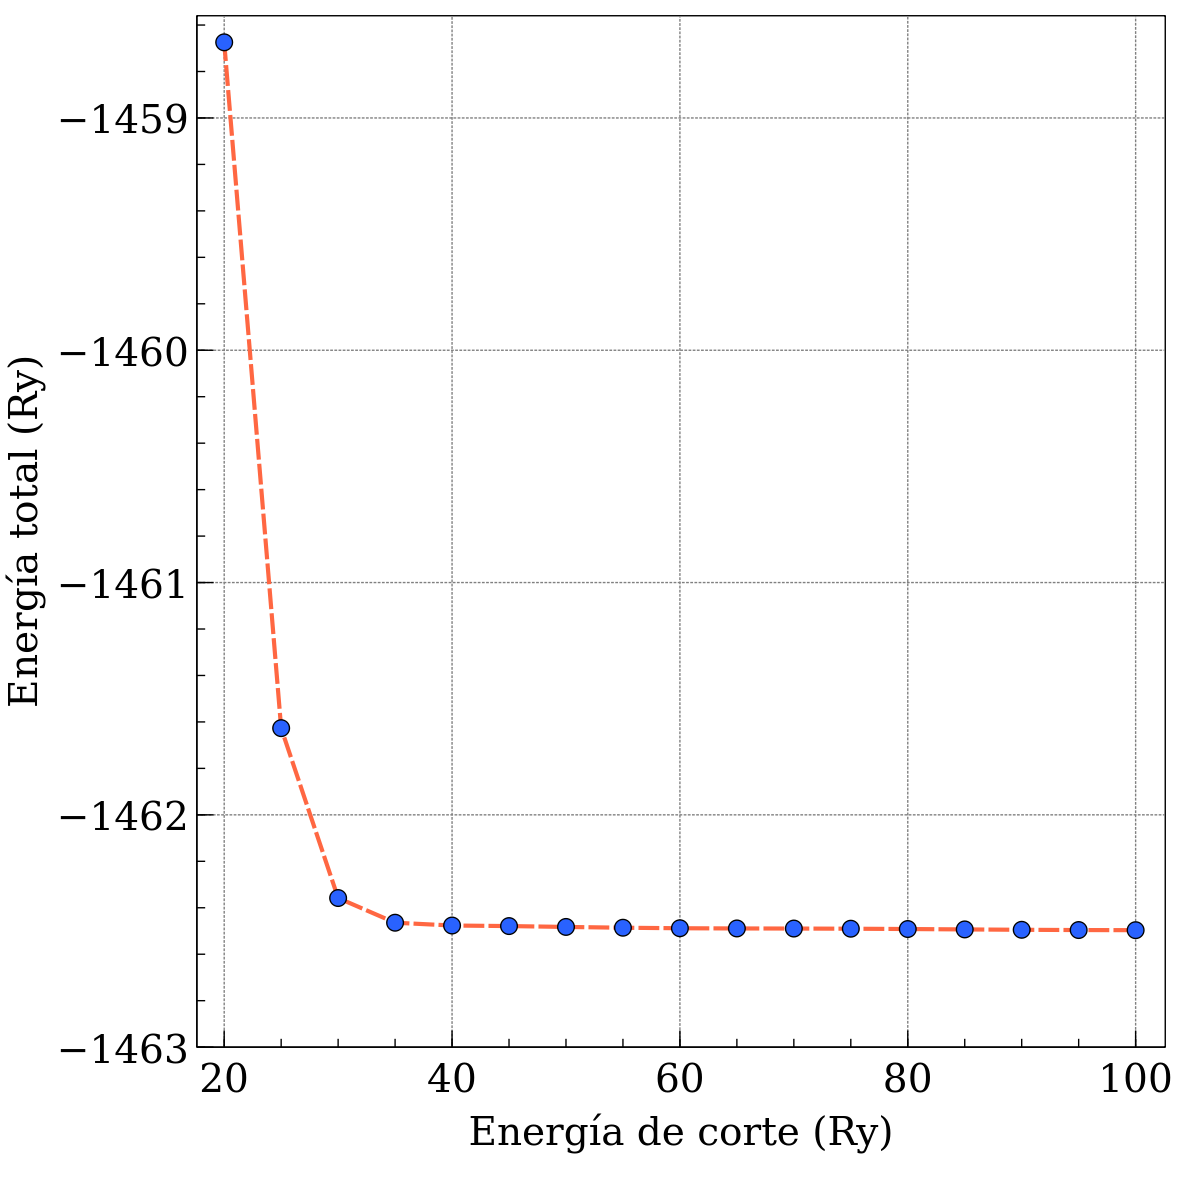
\includegraphics[width=0.7\textwidth]{contenido/resultados/optimizacion/img_optimizacion/energia_corte_YCO.png}
    \caption[Energ\'ia de corte $YCrO_{3}$]{Energ\'ia de corte optima 
        para el $YCrO_{3}$}
    \label{energia_corte_YCO}
\end{figure}

\noindent Como se mencion\'o la energ\'ia de corte es un par\'ametro 
importante. Esto es 
debido a que el conjunto de ondas planas es infinito lo cual es un problema 
para llevar a cabo una simulaci\'on. Este problema se soluciona imponiendo un 
limite en el n\'umero de ondas planas utilizadas, dicho limite es la energ\'ia 
de corte. Es posible considerar ondas planas m\'as all\'a de la energ\'ia de 
corte pero el aumento en la precisi\'on de los resultados es muy peque\~no y no 
justifica el aumento del tiempo de simulaci\'on y de la capacidad de c\'alculo 
computacional requerida para concretar la simulaci\'on.

\subsection{Dimensi\'on de la grilla de puntos K}

Muchas cantidades que necesitamos evaluar involucran integrales sobre la 
primera zona de Brillouin. En la pr\'actica, las integrales se discretizan 
asociando un peso a los puntos K que se consideran.
La dimensi\'on de la grilla de puntos K en la red reciproca debe optimizarse 
con el fin de mejorar la precisi\'on de los 
c\'alculos y reducir el tiempo de simulaci\'on. Para determinar las dimensiones 
\'optimas de la grilla de puntos K para ambos materiales, se realizaron varias 
simulaciones probando varios tama\~nos de grilla. El paquete Quantum Espresso 
implementa el m\'etodo de Monkhorst-Pack para el cual se deben indicar tres 
valores correspondientes a los tres ejes espaciales. Para el $BiFeO_{3}$ se 
utilizaron grillas en el intervalo de $2 \times 2 \times 2$ hasta $9 \times 9 
\times 9$ y para el $YCrO_{3}$ se utilizaron grillas en el rango de $2 \times 2 
\times 2$ hasta $10 \times 10 \times 10$.

\noindent Para el $BiFeO_{3}$ se obtuvo que la grilla optima es de $6 \times 6 
\times 6$, 
como se puede observar en la gr\'afica \ref{puntos_k_BFO}.

\begin{figure}[H]
    \centering
    \includegraphics[width=0.7\textwidth]{contenido/resultados/optimizacion/img_optimizacion/energia_kp_BFO.png}
    \caption[Dimensi\'on de la grilla de puntos k $BiFeO_{3}$]{Dimensi\'on de 
    la grilla de puntos k \'optima para el $BiFeO_{3}$. El eje inferior muestra 
    solo el valor en una dimensi\'on por claridad, dado que la definici\'on 
    real es en tres dimensiones $a \times a \times a$}
    \label{puntos_k_BFO}
\end{figure}

\noindent Para el $YCrO_{3}$ se obtuvo que la grilla \'optima es de $6 \times 6 
\times 6$, 
como se puede observar en la gr\'afica \ref{puntos_k_YCO}.

\begin{figure}[H]
    \centering
    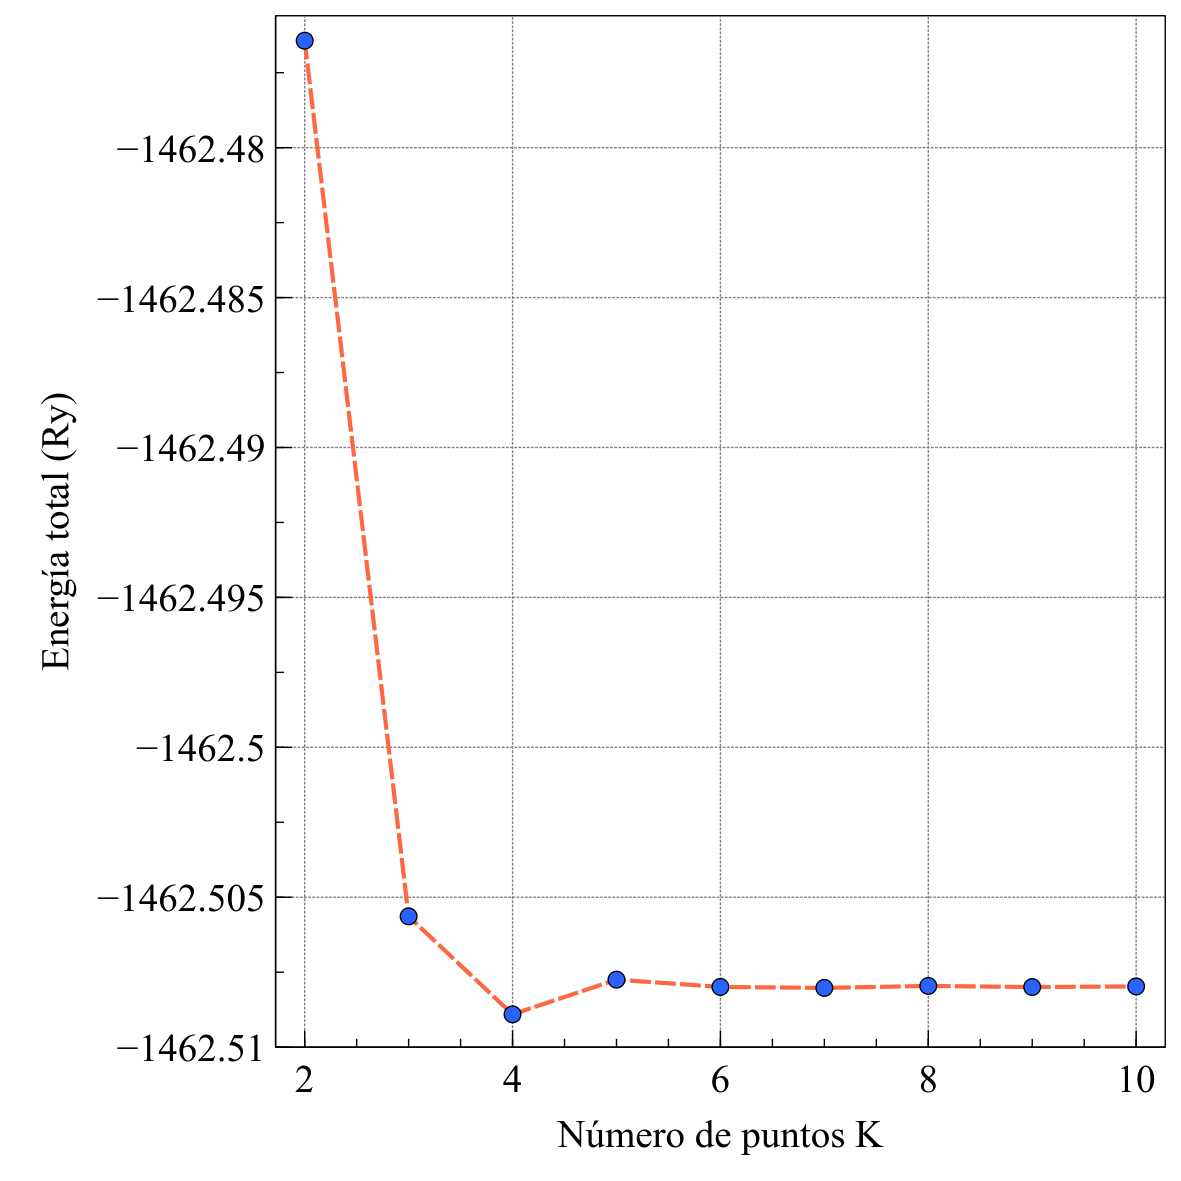
\includegraphics[width=0.7\textwidth]{contenido/resultados/optimizacion/img_optimizacion/energia_kp_YCO.png}
    \caption[Dimensi\'on de la grilla de puntos k $YCrO_{3}$]{Dimensi\'on de 
        la grilla de puntos k \'optima para el $YCrO_{3}$. El eje inferior 
        muestra solo el valor en una dimensi\'on por claridad, dado que la 
        definici\'on real es en tres dimensiones $a \times a \times a$}
    \label{puntos_k_YCO}
\end{figure}


% ---------------------------
% Relajacion
% ---------------------------

\section{Relajaci\'on de la estructura cristalina}
Con el fin de obtener mejores resultados, las estructuras cristalinas 
utilizadas en las simulaciones pasaron por un proceso de relajaci\'on. 
Para los cuales se definieron los siguientes limites de convergencia: 
$10^{-5}$eV para la variaci\'on m\'axima de energ\'ia, $0,03eV$\AA$^{-1}$ 
para la fuerza y $0,05$ Gp para la presi\'on. Este proceso de relajaci\'on se 
realiz\'o para cada arreglo antiferromagn\'etico de cada material utilizado. 
Cada valor mostrado en las gr\'aficas siguientes, es el resultado de un 
c\'alculo de campo autoconsistente en el cual se var\'ian los par\'ametros de 
red, se calcula la energ\'ia total y la fuerza sobre la estructura cristalina. 
Estos pasos de c\'alculo de campo autoconsistente se iteran siendo las 
condiciones iniciales de cada paso las condiciones finales del paso anterior, 
hasta converger con las restricciones antes mencionadas.

\noindent El proceso de relajaci\'on entrega un archivo de texto extenso, que 
contiene 
muchos pasos intermedios de la simulaci\'on junto a los datos de inter\'es. Por 
ello es necesario realizar un procesamiento de este archivo para extraer los 
datos importantes y poder realizar las gr\'aficas de energ\'ia total vs 
iteraci\'on y las gr\'aficas de fuerza vs iteraci\'on. El procesamiento del 
archivo se realiz\'o con un script shell.

\subsection{$\mathbf{BiFeO_{3}}$ con arreglo antiferromagn\'etico tipo A}

\begin{table}[H]
    \begin{center}
        \caption{Comparaci\'on entre los par\'ametros de red antes y despu\'es 
        de la relajaci\'on del $BiFeO_{3}$ con arreglo antiferromagn\'etico 
        tipo A.}
        \begin{tabular}{ccc}
            \hline
               & \textbf{Inicial} \cite{tomar2018} & \textbf{Final} \\
            \hline \hline
            a (\AA) & $5.57$  & $5.65$   \\
            \hline
            c (\AA) & $13.86$ & $14.16$   \\
            \hline
        \end{tabular}
        \singlespace
        \label{bfo_a_ini_fin}
    \end{center}
\end{table}

\noindent La tabla \ref{bfo_a_ini_fin} muestra la comparaci\'on entre los 
par\'ametros de red del $BiFeO_{3}$ con arreglo antiferromagn\'etico tipo A 
antes y despu\'es de la relajaci\'on.

\begin{figure}[H]
    \centering
    \subfloat[]{
        \label{bfo_fuerza_a}
        
        \includegraphics[width=0.5\textwidth]{contenido/resultados/relajacion/img_relajacion/fuerza_BFO_A.png}}
    \subfloat[]{
        \label{bfo_energia_a}
        
        \includegraphics[width=0.5\textwidth]{contenido/resultados/relajacion/img_relajacion/energia_BFO_A.png}}
    \singlespace
    \caption[Minimizaci\'on de la fuerza y la energ\'ia del $BiFeO_{3}$ con 
    arreglo antiferromagn\'etico tipo 
    A]{\ref{minimizacion_bfo_A} \subref{bfo_fuerza_a} Minimizaci\'on de la 
    fuerza sobre la estructura antiferromagn\'etica de tipo A del $BiFeO_{3}$. 
    \ref{minimizacion_bfo_A} \subref{bfo_energia_a} Minimizaci\'on de la 
    energ\'ia de la estructura antiferromagn\'etica de tipo A del $BiFeO_{3}$.}
    \label{minimizacion_bfo_A}
\end{figure}

\noindent La figura \ref{minimizacion_bfo_A} muestra la minimizaci\'on de la 
fuerza \ref{minimizacion_bfo_A} \subref{bfo_fuerza_a} y de la energ\'ia 
\ref{minimizacion_bfo_A} \subref{bfo_energia_a} del $BiFeO_{3}$ con arreglo 
antiferromagn\'etico tipo A. Se puede observar que el sistema converge luego de 
10 iteraciones.

\subsection{$\mathbf{BiFeO_{3}}$ con arreglo antiferromagn\'etico tipo G}

\begin{table}[H]
    \begin{center}
        \caption{Comparaci\'on entre los par\'ametros de red antes y despu\'es 
            de la relajaci\'on del $BiFeO_{3}$ con arreglo antiferromagn\'etico 
            tipo G.}
        \begin{tabular}{ccc}
            \hline
            & \textbf{Inicial} \cite{tomar2018} & \textbf{Final} \\
            \hline \hline
            a (\AA) & $5.57$  & $5.64$   \\
            \hline
            c (\AA) & $13.86$ & $14.07$   \\
            \hline
        \end{tabular}
        \singlespace
        \label{bfo_g_ini_fin}
    \end{center}
\end{table}

\noindent La tabla \ref{bfo_g_ini_fin} muestra la comparaci\'on entre los 
par\'ametros de red del $BiFeO_{3}$ con arreglo antiferromagn\'etico tipo G 
antes y despu\'es de la relajaci\'on.

\begin{figure}[H]
    \centering
    \subfloat[]{
        \label{bfo_fuerza_g}
        
        \includegraphics[width=0.5\textwidth]{contenido/resultados/relajacion/img_relajacion/fuerza_BFO_G.png}}
    \subfloat[]{
        \label{bfo_energia_g}
        
        \includegraphics[width=0.5\textwidth]{contenido/resultados/relajacion/img_relajacion/energia_BFO_G.png}}
    \singlespace
    \caption[Minimizaci\'on de la fuerza y la energ\'ia del $BiFeO_{3}$ con 
    arreglo antiferromagn\'etico tipo 
    G]{\ref{minimizacion_bfo_G} \subref{bfo_fuerza_g} Minimizaci\'on de la 
        fuerza sobre la estructura antiferromagn\'etica de tipo G del 
        $BiFeO_{3}$. 
        \ref{minimizacion_bfo_G} \subref{bfo_energia_g} Minimizaci\'on de la 
        energ\'ia de la estructura antiferromagn\'etica de tipo G del 
        $BiFeO_{3}$.}
    \label{minimizacion_bfo_G}
\end{figure}

\noindent La figura \ref{minimizacion_bfo_G} muestra la minimizaci\'on de la 
fuerza \ref{minimizacion_bfo_G} \subref{bfo_fuerza_g} y de la energ\'ia 
\ref{minimizacion_bfo_G} \subref{bfo_energia_g} del $BiFeO_{3}$ con arreglo 
antiferromagn\'etico tipo G. Se puede observar que el sistema converge luego de 
9 iteraciones.

\subsection{$\mathbf{YCrO_{3}}$ con arreglo antiferromagn\'etico tipo A}

\begin{table}[H]
    \begin{center}
        \caption{Comparaci\'on entre los par\'ametros de red antes y despu\'es 
            de la relajaci\'on del $YCrO_{3}$ con arreglo antiferromagn\'etico 
            tipo A.}
        \begin{tabular}{ccc}
            \hline
            & \textbf{Inicial} \cite{geller1956} & \textbf{Final} \\
            \hline \hline
            a (\AA) & $5.247$  & $5.14$   \\
            \hline
            b (\AA) & $5.518$ & $5.49$   \\
            \hline
            c (\AA) & $7.54$ & $7.41$   \\
            \hline
        \end{tabular}
        \singlespace
        \label{yco_a_ini_fin}
    \end{center}
\end{table}

\noindent La tabla \ref{yco_a_ini_fin} muestra la comparaci\'on entre los 
par\'ametros de red del $YCrO_{3}$ con arreglo antiferromagn\'etico tipo A 
antes y despu\'es de la relajaci\'on.

\begin{figure}[H]
    \centering
    \subfloat[]{
        \label{yco_fuerza_a}
        
        \includegraphics[width=0.5\textwidth]{contenido/resultados/relajacion/img_relajacion/fuerza_YCO_A.png}}
    \subfloat[]{
        \label{yco_energia_a}
        
        \includegraphics[width=0.5\textwidth]{contenido/resultados/relajacion/img_relajacion/energia_YCO_A.png}}
    \singlespace
    \caption[Minimizaci\'on de la fuerza y la energ\'ia del $YCrO_{3}$ con 
    arreglo antiferromagn\'etico tipo 
    A]{\ref{minimizacion_yco_A} \subref{yco_fuerza_a} Minimizaci\'on de la 
        fuerza sobre la estructura antiferromagn\'etica de tipo A del 
        $YCrO_{3}$. 
        \ref{minimizacion_yco_A} \subref{yco_energia_a} Minimizaci\'on de la 
        energ\'ia de la estructura antiferromagn\'etica de tipo A del 
        $YCrO_{3}$.}
    \label{minimizacion_yco_A}
\end{figure}

\noindent La figura \ref{minimizacion_yco_A} muestra la minimizaci\'on de la 
fuerza \ref{minimizacion_yco_A} \subref{yco_fuerza_a} y de la energ\'ia 
\ref{minimizacion_yco_A} \subref{yco_energia_a} del $YCrO_{3}$ con arreglo 
antiferromagn\'etico tipo A. Se puede observar que el sistema converge luego de 
14 iteraciones.


\subsection{$\mathbf{YCrO_{3}}$ con arreglo antiferromagn\'etico tipo C}

\begin{table}[H]
    \begin{center}
        \caption{Comparaci\'on entre los par\'ametros de red antes y despu\'es 
            de la relajaci\'on del $YCrO_{3}$ con arreglo antiferromagn\'etico 
            tipo C.}
        \begin{tabular}{ccc}
            \hline
            & \textbf{Inicial} \cite{geller1956} & \textbf{Final} \\
            \hline \hline
            a (\AA) & $5.247$  & $5.15$   \\
            \hline
            b (\AA) & $5.518$ & $5.47$   \\
            \hline
            c (\AA) & $7.54$ & $7.42$   \\
            \hline
        \end{tabular}
        \singlespace
        \label{yco_c_ini_fin}
    \end{center}
\end{table}

\noindent La tabla \ref{yco_c_ini_fin} muestra la comparaci\'on entre los 
par\'ametros de red del $YCrO_{3}$ con arreglo antiferromagn\'etico tipo C 
antes y despu\'es de la relajaci\'on.

\begin{figure}[H]
    \centering
    \subfloat[]{
        \label{yco_fuerza_c}
        
        \includegraphics[width=0.5\textwidth]{contenido/resultados/relajacion/img_relajacion/fuerza_YCO_C.png}}
    \subfloat[]{
        \label{yco_energia_c}
        
        \includegraphics[width=0.5\textwidth]{contenido/resultados/relajacion/img_relajacion/energia_YCO_C.png}}
    \singlespace
    \caption[Minimizaci\'on de la fuerza y la energ\'ia del $YCrO_{3}$ con 
    arreglo antiferromagn\'etico tipo 
    C]{\ref{minimizacion_yco_C} \subref{yco_fuerza_c} Minimizaci\'on de la 
        fuerza sobre la estructura antiferromagn\'etica de tipo C del 
        $YCrO_{3}$. 
        \ref{minimizacion_yco_C} \subref{yco_energia_c} Minimizaci\'on de la 
        energ\'ia de la estructura antiferromagn\'etica de tipo C del 
        $YCrO_{3}$.}
    \label{minimizacion_yco_C}
\end{figure}

\noindent La figura \ref{minimizacion_yco_C} muestra la minimizaci\'on de la 
fuerza \ref{minimizacion_yco_C} \subref{yco_fuerza_c} y de la energ\'ia 
\ref{minimizacion_yco_C} \subref{yco_energia_c} del $YCrO_{3}$ con arreglo 
antiferromagn\'etico tipo C. Se puede observar que el sistema converge luego de 
12 iteraciones.


\subsection{$\mathbf{YCrO_{3}}$ con arreglo antiferromagn\'etico tipo G}

\begin{table}[H]
    \begin{center}
        \caption{Comparaci\'on entre los par\'ametros de red antes y despu\'es 
            de la relajaci\'on del $YCrO_{3}$ con arreglo antiferromagn\'etico 
            tipo G.}
        \begin{tabular}{ccc}
            \hline
            & \textbf{Inicial} \cite{geller1956} & \textbf{Final} \\
            \hline \hline
            a (\AA) & $5.247$  & $5.14$   \\
            \hline
            b (\AA) & $5.518$ & $5.47$   \\
            \hline
            c (\AA) & $7.54$ & $7.41$   \\
            \hline
        \end{tabular}
        \singlespace
        \label{yco_g_ini_fin}
    \end{center}
\end{table}

\noindent La tabla \ref{yco_g_ini_fin} muestra la comparaci\'on entre los 
par\'ametros de red del $YCrO_{3}$ con arreglo antiferromagn\'etico tipo G 
antes y despu\'es de la relajaci\'on.

\begin{figure}[H]
    \centering
    \subfloat[]{
        \label{yco_fuerza_g}
        
        \includegraphics[width=0.5\textwidth]{contenido/resultados/relajacion/img_relajacion/fuerza_YCO_G.png}}
    \subfloat[]{
        \label{yco_energia_g}
        
        \includegraphics[width=0.5\textwidth]{contenido/resultados/relajacion/img_relajacion/energia_YCO_G.png}}
    \singlespace
    \caption[Minimizaci\'on de la fuerza y la energ\'ia del $YCrO_{3}$ con 
    arreglo antiferromagn\'etico tipo 
    G]{\ref{minimizacion_yco_G} \subref{yco_fuerza_g} Minimizaci\'on de la 
        fuerza sobre la estructura antiferromagn\'etica de tipo G del 
        $YCrO_{3}$. 
        \ref{minimizacion_yco_G} \subref{yco_energia_g} Minimizaci\'on de la 
        energ\'ia de la estructura antiferromagn\'etica de tipo G del 
        $YCrO_{3}$.}
    \label{minimizacion_yco_G}
\end{figure}

\noindent La figura \ref{minimizacion_yco_G} muestra la minimizaci\'on de la 
fuerza \ref{minimizacion_yco_G} \subref{yco_fuerza_g} y de la energ\'ia 
\ref{minimizacion_yco_G} \subref{yco_energia_g} del $YCrO_{3}$ con arreglo 
antiferromagn\'etico tipo G. Se puede observar que el sistema converge luego de 
13 iteraciones.


% -------------------
% Ferrita de bismuto
% -------------------

\section{Par\'ametros estructurales, bandas de energ\'ia , densidad de estados 
y densidad de carga del $\mathbf{BiFeO_{3}}$}
\subsection{Par\'ametros estructurales del $\mathbf{BiFeO_{3}}$ con arreglos 
antiferromagn\'eticos tipo A y G}

La tabla \ref{tabla_BiFeO3_parametro_red} muestra los par\'ametros 
estructurales (a, c) de la red hexagonal del $BiFeO_{3}$ en el espacio de grupo 
R3c (\#161) para los dos arreglos antiferromagn\'eticos. Los par\'ametros se 
obtuvieron de la relajaci\'on de la estructura cristalina. Los valores 
obtenidos se encuentran en concordancia con resultados experimentales 
\cite{lu2010}, y te\'oricos obtenidos con DFT 
\cite{lee2012,arnold2015}.

% ------------------------------
% TABLA: parametros optimizados
% ------------------------------

\begin{table}[H]
    \begin{center}
        \caption[Par\'ametros de red optimizados del 
        $BiFeO_{3}$]{Comparaci\'on 
            de los par\'ametros estructurales de los dos arreglos 
            antiferromagn\'eticos, con valores obtenidos de 
            difracci\'on de 
            rayos X y DFT}
        \begin{tabular}{ccc}
            \hline
                 & \textbf{a (\AA)} & \textbf{c (\AA)} \\
            \hline \hline
            AF-A & $5.65$ & $14.16$ \\
            \hline
            AF-G & $5.64$ & $14.07$ \\
            \hline
            \cite{lu2010} & $5.58$ & $13.90$ \\
            \hline
            \cite{lee2012} & $5.6143$ & $13.98$ \\
            \hline
            \cite{arnold2015} & $5.5725$ & $13.85$ \\
            \hline
        \end{tabular}
        \label{tabla_BiFeO3_parametro_red}
    \end{center}
\end{table}

\noindent Los par\'ametros estructurales de menor valor pertenecen al arreglo 
antiferromagn\'etico tipo G, y la tabla 
\ref{tabla_BiFeO3_ener_vol_mag} muestra 
que 
posee la menor energ\'ia total y el menor volumen. Por lo tanto el 
arreglo 
antiferromagn\'etico tipo G es el m\'as estable.

% 
%------------------------------------------------------------------------
% TABLA: energia total, volumen de la celda, momento magnetico del 
%hierro
% 
%------------------------------------------------------------------------

\begin{table}[H]
    \begin{center}
        \caption{Energ\'ia total, volumen de la celda y momento 
            magn\'etico del 
            \'atomo de hierro,
            para el $BiFeO_{3}$ con los arreglos antiferromagn\'eticos tipo A y 
            G}
        \begin{tabular}{cccc}
            \hline
            \textbf{Tipo} & \textbf{Energ\'ia total (Ry)} & 
            \textbf{Volumen 
                (\AA $^{3}$)} & \textbf{Momento magn\'etico Fe ($\mu 
                _{B}$)}\\
            \hline \hline
            AF-A & $-3194.656$ & $391.58$ & $4.19$ \\
            \hline
            AF-G & $-3194.725$ & $387.55$ & $4.05$ \\
            \hline
        \end{tabular}
        \singlespace
        \label{tabla_BiFeO3_ener_vol_mag}
    \end{center}
\end{table}

\noindent Los momentos magn\'eticos del hierro de los dos arreglos 
antiferromagn\'eticos 
mostrados en la tabla \ref{tabla_BiFeO3_ener_vol_mag} se encuentran en 
concordancia con los datos experimentales de $3.75$ $\mu _{B}$ 
\cite{fischer1980} 
y $4.0$ $\mu _{B}$ \cite{sosnowska2002}. Las diferencias entre los resultados 
obtenidos y los datos experimentales pueden ser atribuidos a varios factores, 
tales como temperatura y posibles defectos de formaci\'on en las muestras de 
$BiFeO_{3}$ y en el caso de los datos obtenidos con DFT, puede deberse a como 
se encuentra implementado el m\'etodo de DFT + U en los distintos paquetes de 
simulaci\'on utilizados en dichos estudios.

\subsection{Estructura de bandas de energ\'ia del $\mathbf{BiFeO_{3}}$ con 
arreglo antiferromagn\'etico tipo A}

% ###########################################################
% ###########################################################
%                  INICIO TIPO A
% ###########################################################
% ###########################################################

% ----------------------------
% FIGURA: banda BiFeO3 tipo A
% ----------------------------

\begin{figure}[H]
    \centering
    
    \includegraphics[width=0.7\textwidth]{contenido/resultados/ferrita_bismuto/img_ferrita_bismuto/BiFeO3_bandas_A_inf.png}
    \singlespace
    \caption[Bandas de energ\'ia del $BiFeO_{3}$ con arreglo 
    antiferromagn\'etico tipo A]{Estructura de bandas de energ\'ia del 
        $BiFeO_{3}$ con arreglo antiferromagn\'etico tipo A. La l\'inea roja 
        marca el 
        nivel de fermi. Los puntos de alta simetr\'ia tomados en la primera 
        zona de 
        brillouin son $\Gamma - M - K - \Gamma$.}
    \label{bfo_band_a}
\end{figure}

En la figura \ref{bfo_band_a} se observan las bandas de energ\'ia del arreglo 
antiferromagn\'etico tipo A del $BiFeO_{3}$. Las energ\'ias fueron escaladas 
respecto al nivel de fermi, que es tomado como el cero de la escala vertical. 
La estructura de bandas muestra un 
gap de 
energ\'ia alrededor del nivel de fermi, definido entre el nivel de energ\'ia 
m\'as alto de la banda de valencia ubicado en el punto $\Gamma$ y el nivel de 
energ\'ia m\'as bajo de la banda de conducci\'on ubicado entre los puntos $K - 
\Gamma$. El gap de energ\'ia es de $1.4$ eV el cual es cercano al valor de 
$1.3$ eV 
reportado por otros estudios \cite{ju2009,gujar2007}. En la banda de 
conducci\'on se observa una secci\'on alrededor del nivel de energ\'ia de $1.5$ 
eV que no posee bandas; de esta forma se pueden distinguir dos grupos de 
bandas. El grupo m\'as cercano al nivel de fermi es bastante denso, y el m\'as 
alejado no tanto. La banda de valencia en contraste es compacta.

\subsection{Densidad de estados del $\mathbf{BiFeO_{3}}$ con arreglo 
antiferromagn\'etico tipo A}

% -------------------------------------------
% FIGURA: densidades de estado BIFeO3 tipo G
% -------------------------------------------

\begin{figure}
    \centering
    \subfloat[]{
        \label{bfo_tot_a}
        
        \includegraphics[width=0.5\textwidth]{contenido/resultados/ferrita_bismuto/img_ferrita_bismuto/BiFeO3_DOS_A_inf.png}}
    \subfloat[]{
        \label{bfo_bi_a}
        
        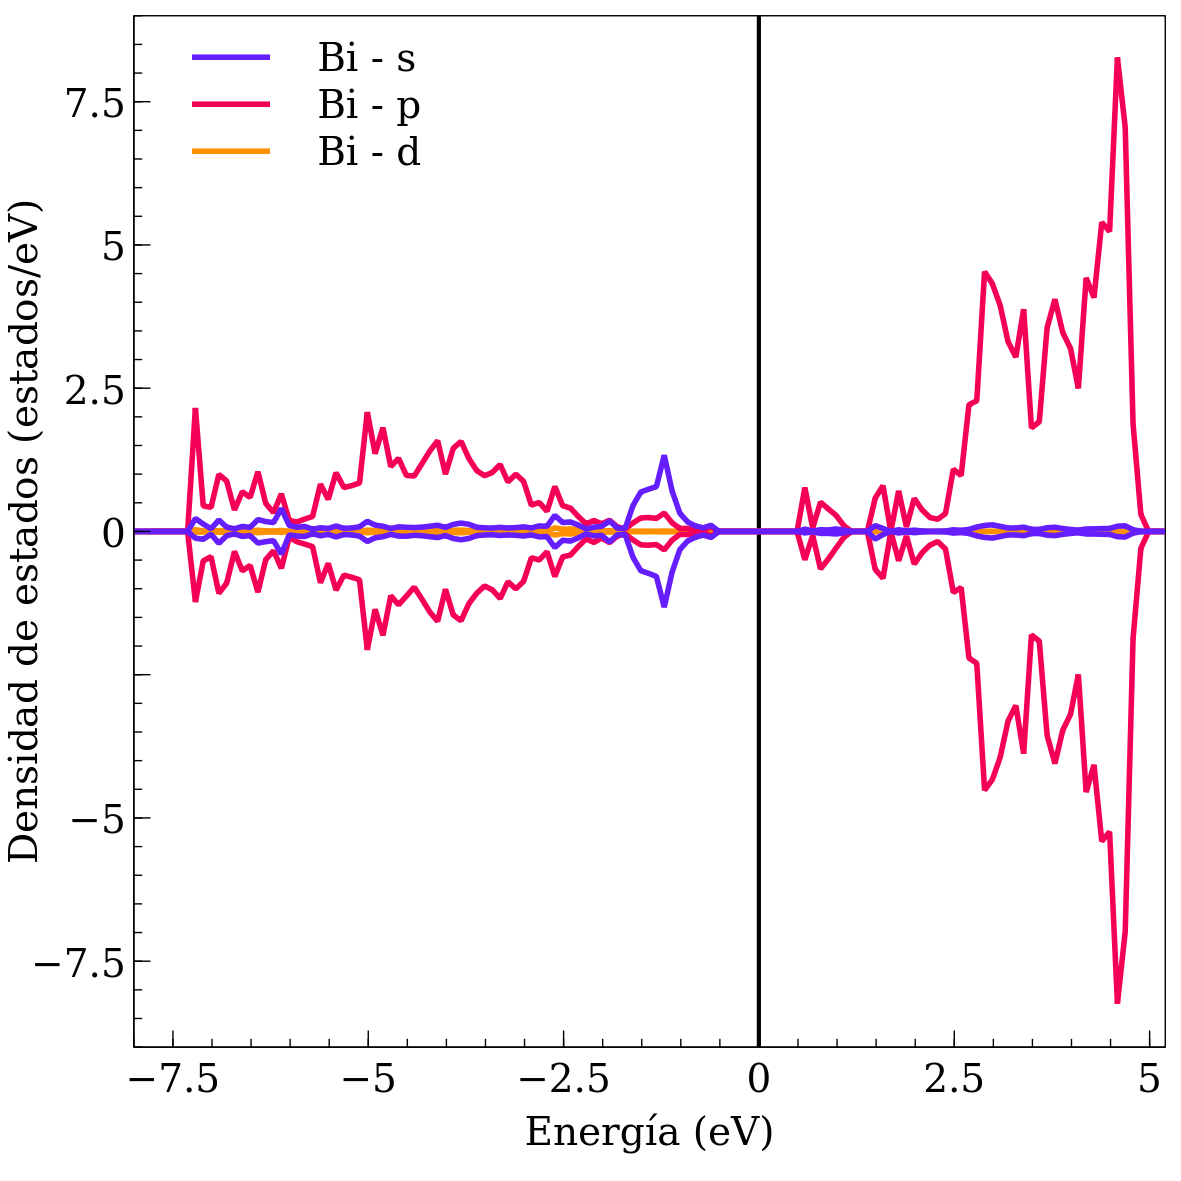
\includegraphics[width=0.5\textwidth]{contenido/resultados/ferrita_bismuto/img_ferrita_bismuto/BiFeO3_DOS_Bi_A_inf.png}}
    
    \subfloat[]{
        \label{bfo_fe_a}
        
        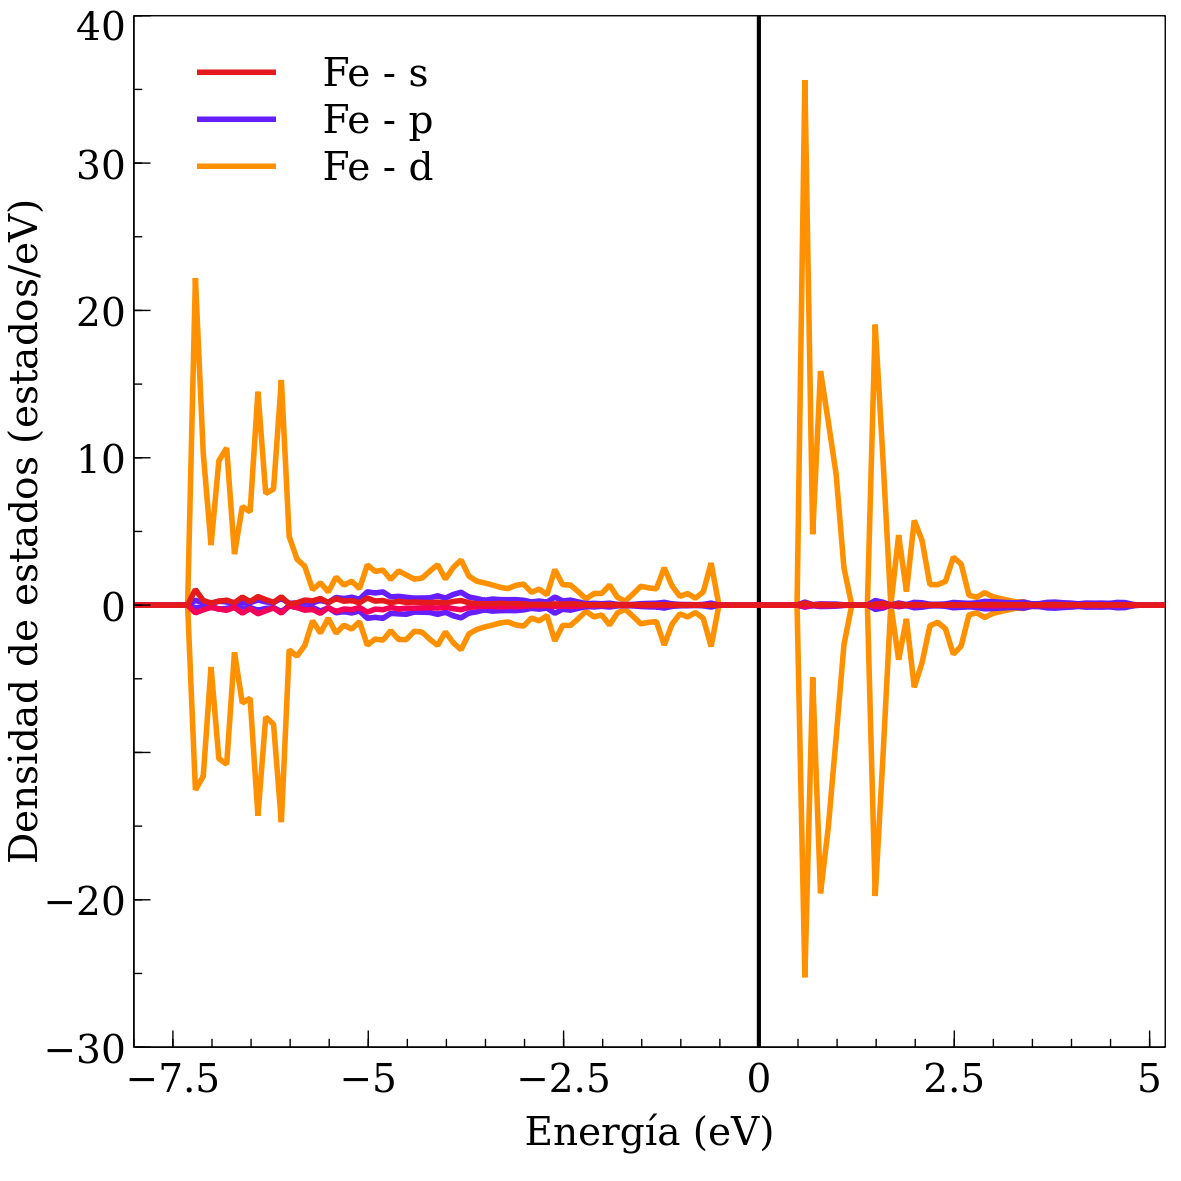
\includegraphics[width=0.5\textwidth]{contenido/resultados/ferrita_bismuto/img_ferrita_bismuto/BiFeO3_DOS_Fe_A_inf.png}}
    \subfloat[]{
        \label{bfo_o_a}
        
        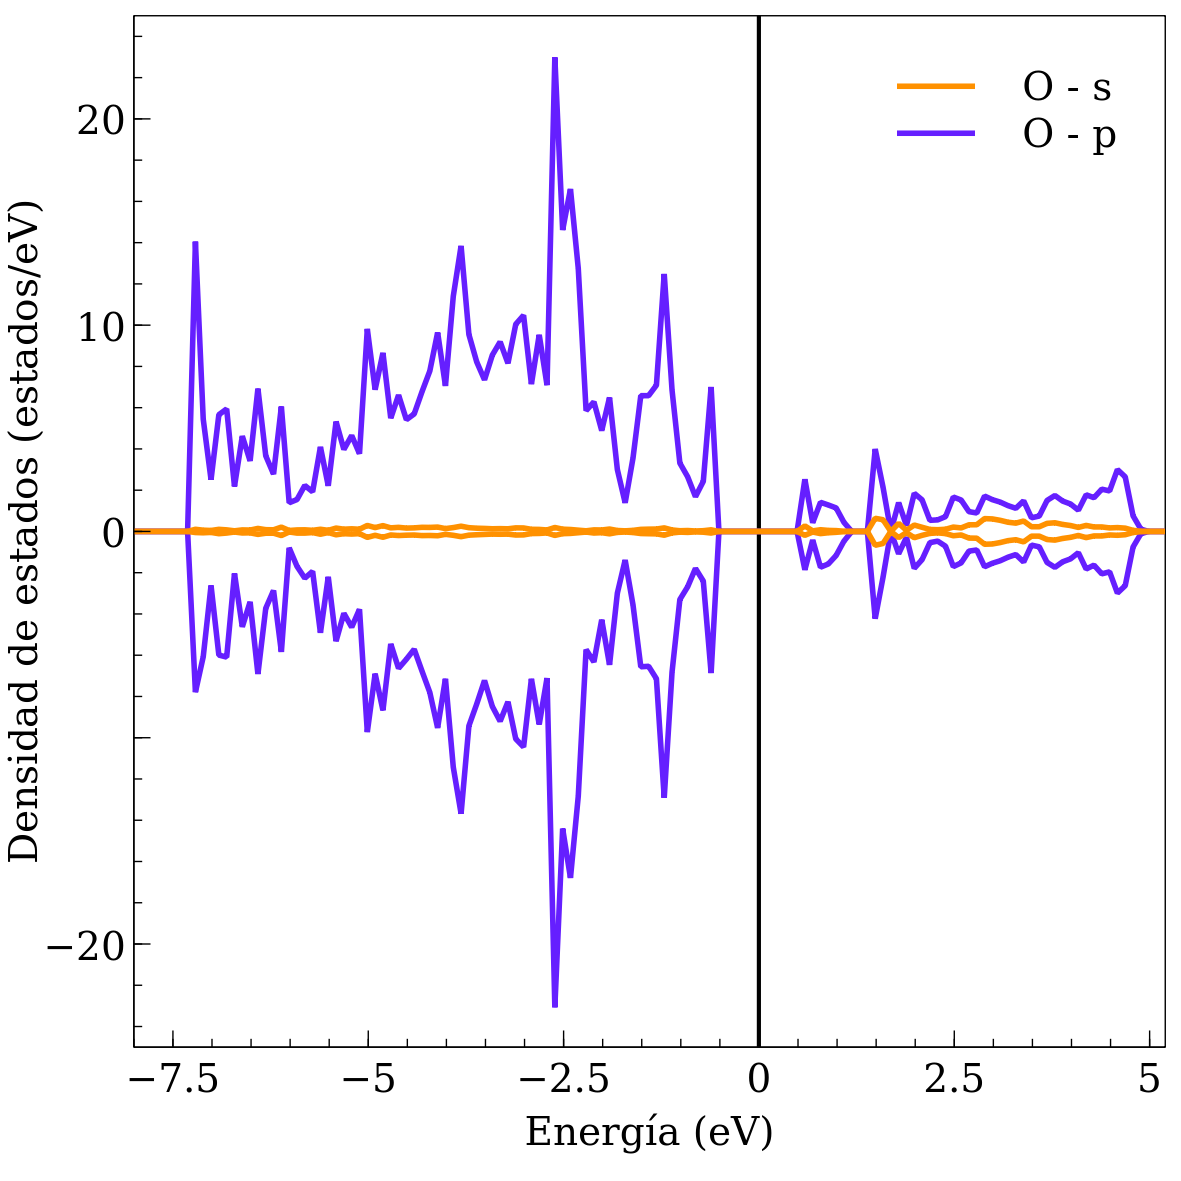
\includegraphics[width=0.5\textwidth]{contenido/resultados/ferrita_bismuto/img_ferrita_bismuto/BiFeO3_DOS_O_A_inf.png}}
    \singlespace
    \caption[Densidad de estados del $BiFeO_{3}$ con arreglo 
    antiferromagn\'etico tipo A]{Densidad de estados del $BiFeO_{3}$ 
    con 
        arreglo antiferromagn\'etico tipo A. La linea negra en cero 
        indica el 
        nivel 
        de fermi. \ref{bfo_dos_a} \subref{bfo_tot_a} Densidad de estados total 
        y de cada elemento. 
        \ref{bfo_dos_a} \subref{bfo_bi_a} 
        Densidad de 
        estados para los orbitales s, p, d del bismuto. \ref{bfo_dos_a} 
        \subref{bfo_fe_a} Densidad 
        de estados 
        para los orbitales s, p ,d del hierro. \ref{bfo_dos_a} \subref{bfo_o_a} 
        Densidad de estados 
        para los 
        orbitales s, p del ox\'igeno.}
    \label{bfo_dos_a}
\end{figure}

% mmmmmmmmmmmmmmmmmmmmmmmmmmmmmmmmmmmmmmmmmmmmmmmmmmmmmmmmmmmmmmmm
%mmmmmmmmmmmmmmmmmmmmmmmmmmmmmmmmmmmmmmmmmmmmmmmmmmmmmmmmmmmmmmmmmmm
%mmmmmmmmmmmmmmmmmmmmmmmmmmmmmmmmmmmmmmmmmmmmmmmmmmmmmmmmmmmmmmmmmmmmm



La figura \ref{bfo_dos_a} \subref{bfo_tot_a} muestra la densidad de estados 
total para cada 
elemento que compone el $BiFeO_{3}$.Las energ\'ias fueron escaladas respecto al 
nivel de fermi que se tomo como cero de la escala horizontal, y la escala 
vertical positiva y negativa corresponden a los espines up y down 
respectivamente. En la banda de conducci\'on cerca del 
nivel de fermi observamos una densidad total de aproximadamente 40 estados/eV 
formada en su mayor\'ia por estados del hierro, seguida de peque\~nas 
contribuciones de bismuto y oxigeno. Tambi\'en podemos observar una secci\'on 
donde no existen estados de ning\'un elemento seguida de una densidad total de 
aproximadamente 25 estados/eV principalmente de hierro, seguido de oxigeno y 
bismuto. A partir del nivel de energ\'ia de 2 eV la densidad de estados total 
cae por debajo de 10 estados/eV , siendo el hierro dominante en el rango de 
2 eV a $2.5$ eV, pasado este nivel los estados de hierro son casi inexistentes, 
y 
el bismuto pasa a predominar manteniendo una densidad de estados por debajo de 
los 5 estados/eV hasta el nivel de 4 eV y elev\'andose hasta aproximadamente 8 
estados/eV alrededor de los $4.5$ eV.Por su parte la densidad de estados del 
oxigeno se mantiene por debajo de los 5 estados/eV sin cambios grandes. 
En la banda de valencia hasta el nivel de energ\'ia de -5 eV los estados de 
oxigeno poseen la mayor densidad de estados totales, fluctuando entre 5 
estados/ev y 25 estados/eV, y por debajo de los 5 estados/eV en el mismo rango 
de energ\'ia se encuentran estados de hierro seguidos por estados de bismuto. A 
partir de los -5 eV la densidad de estados de hierro supera a los otros 
elementos alcanzando aproximadamente los 25 estados/eV en su punto m\'as alto 
en el nivel de -7 eV seguido por los estados de oxigeno que se encuentran entre 
2 estados/eV y 15 estados/eV; y los estados de bismuto poseen una densidad de 
estados por debajo de 3 estados/eV.

% ===============================================
% ===============================================

\noindent La figura \ref{bfo_dos_a} \subref{bfo_bi_a} muestra la densidad de 
estados parcial del 
bismuto 
para cada uno de los orbitales \textbf{s}, \textbf{p} y \textbf{d}. Las 
energ\'ias fueron escaladas respecto al 
nivel de fermi que se tomo como cero de la escala horizontal, y la escala 
vertical positiva y negativa corresponden a los espines up y down 
respectivamente. En la banda 
de conducci\'on hasta el  nivel de energ\'ia de $2.5$ eV la densidad de estados 
se encuentra por debajo de 2 estados/eV y esta formada principalmente 
por el orbital \textbf{p} siendo casi inexistentes los orbitales \textbf{s} y 
\textbf{d}. A partir del nivel de energ\'ia de $2.5$ eV la densidad de estados 
fluct\'ua entre 2 estados/eV y 8 estados/eV, encontr\'andose su punto m\'as 
alto cerca del nivel de energ\'ia de 5 eV; en este rango de energ\'ia el 
orbital \textbf{p} sigue siendo el que m\'as contribuye en comparaci\'on a los 
orbitales \textbf{s} y \textbf{d}. En la banda de valencia se observa que hasta 
el nivel de energ\'ia de -2 eV el orbital \textbf{s} es el de mayor densidad, 
seguido por el orbital \textbf{p}, y la densidad de los orbitales \textbf{d} es 
pr\'acticamente cero. A partir del nivel de energ\'ia de $-2.5$ eV la densidad 
del orbital \textbf{p} pasa a ser la m\'as alta, alcanzando su m\'aximo en el 
nivel de enrg\'ia de $-7.5$ eV con 2 estados/eV. Adem\'as se puede observar que 
en el nivel de energ\'ia de -6 eV las densidades de estados de todos los 
orbitales se reducen casi a cero.

% -------------------------------------------------------------
% FIGURA: densidad de estado parcial hierro del BIFeO3 tipo A
% -------------------------------------------------------------

\noindent La figura \ref{bfo_dos_a} \subref{bfo_fe_a} muestra la densidad de 
estados parcial del 
hierro para 
cada uno de los orbitales \textbf{s}, \textbf{p} y \textbf{d}. Las energ\'ias 
fueron escaladas respecto al 
nivel de fermi que se tomo como cero de la escala horizontal, y la escala 
vertical positiva y negativa corresponden a los espines up y down 
respectivamente. En la banda de 
conducci\'on se observa que hasta el nivel de energ\'ia de 1 eV la densidad del 
orbital \textbf{d} es la m\'as alta alcanzando como m\'aximo los 35 estados/eV, 
y las densidades de los otros orbitales son casi inexistentes. A partir de 1 eV 
existe un peque\~no rango de energ\'ia donde las densidades de los orbitales 
son 
pr\'acticamente cero, luego de ese punto hasta el nivel de energ\'ia de $2.5$ 
eV 
la densidad del orbital \textbf{d} sigue siendo la m\'as alta, alcanzando como 
m\'aximo 20 estados/eV. A partir de los $2.5$ eV las densidades de los 
orbitales 
caen a cero. En la banda de valencia hasta el nivel de energ\'ia de $-5.5$ eV 
la 
densidad del orbital \textbf{d} es la m\'as alta manteni\'endose por debajo de 
4 estados/eV y las densidades de los otros orbitales son casi cero. A partir de 
$-5.5$ eV la densidad del orbital \textbf{d} sigue siendo la m\'as alta pero 
elev\'andose respecto al intervalo anterior, alcanzando su m\'aximo en $-7.5$ 
eV 
con 20 estados/eV, y los otros orbitales contin\'uan con una densidad casi 
inexistente.

% --------------------------------------------------------------
% FIGURA: densidad de estado parcial oxigeno del BIFeO3 tipo A
% --------------------------------------------------------------

\noindent La figura \ref{bfo_dos_a} \subref{bfo_o_a} muestra la densidad de 
estados parcial del 
ox\'igeno, 
para cada uno de los orbitales \textbf{s} y \textbf{p}. Las energ\'ias 
fueron escaladas respecto al 
nivel de fermi que se tomo como cero de la escala horizontal, y la escala 
vertical positiva y negativa corresponden a los espines up y down 
respectivamente. En la banda de conducci\'on se observa que hasta 
aproximadamente 1 eV la densidad del orbital \textbf{p} es la m\'as alta, 
estando por debajo de 2 estados/eV y la densidad del orbital \textbf{s} es casi 
inexistente. A partir de este punto existe un rango de energ\'ia corto donde 
las densidades de ambos orbitales son cero. Luego de este rango la densidad del 
estado \textbf{p} continua por sobre la del orbital \textbf{s} pero por debajo 
de 4 estados/eV. En la banda de valencia se observa que la densidad del orbital 
\textbf{p} es la m\'as alta y la densidad del orbital \textbf{s} es 
pr\'acticamente cero. La densidad del orbital \textbf{p} es de aproximadamente 
6 estados/eV alrededor del nivel de energ\'ia $-0.5$ eV , elev\'andose hasta 10 
estados/eV alrededor del nivel de energ\'ia de -1 eV, luego se reduce por 
debajo de 2 estados/eV cerca del nivel de -2 eV para luego alcanzar su m\'aximo 
con 22 estados/eV en el nivel de energ\'ia $-2.5$ eV. Pasado este punto se va 
reduciendo hasta alcanzar un m\'inimo de 2 estados/eV en el nivel de energ\'ia 
de -6 eV, y luego se eleva hasta alcanzar 12 estados/eV en $-7.5$ eV.


% ###########################################################
% ###########################################################
%                  INICIO TIPO G
% ###########################################################
% ###########################################################

\subsection{Estructura de bandas de energ\'ia del $\mathbf{BiFeO_{3}}$ con      
arreglo antiferromagn\'etico tipo G}

% ----------------------------
% FIGURA: banda BiFeO3 tipo G
% ----------------------------

\begin{figure}[H]
    \centering
    
    \includegraphics[width=0.7\textwidth]{contenido/resultados/ferrita_bismuto/img_ferrita_bismuto/BiFeO3_bandas_G_inf.png}
    \singlespace
    \caption[Bandas de energ\'ia del $BiFeO_{3}$ con arreglo 
    antiferromagn\'etico tipo G]{Estructura de bandas de energ\'ia del 
        $BiFeO_{3}$ con arreglo antiferromagn\'etico tipo G. La l\'inea roja 
        marca el 
        nivel de fermi. Los puntos de alta simetr\'ia tomados en la primera 
        zona de 
        brillouin son $\Gamma - M - K - \Gamma$.}
    \label{bfo_band_g}
\end{figure}


La figura \ref{bfo_band_g} muestra la estructura de bandas de energ\'ia del 
$BiFeO_{3}$ con arreglo antiferromagn\'etico tipo G. Las energ\'ias 
fueron escaladas respecto al nivel de fermi, que es tomado como el 
cero de la escala vertical. Se observa que el gap de 
energ\'ia es de $1.8$ eV el cual es cercano al valor de $1.9$ eV reportado por 
otros estudios \cite{ju2009,lee2012}. El gap se halla entre el m\'inimo de la 
banda de conducci\'on ubicado entre los puntos $K - \Gamma$ y el m\'aximo de la 
banda de valencia ubicado entre los puntos $K - \Gamma$. En la banda de 
conducci\'on se observa alrededor del nivel de energ\'ia de 1 eV una zona sin 
bandas de energ\'ia, de modo similar por sobre los 2 eV existe una zona muy 
estrecha que no presenta bandas de energ\'ia.

\subsection{Densidad de estados del $\mathbf{BiFeO_{3}}$ con arreglo      
antiferromagn\'etico tipo G}

% -------------------------------------------
% FIGURA: densidades de estado BIFeO3 tipo G
% -------------------------------------------

\begin{figure}[H]
    \centering
    \subfloat[]{
        \label{bfo_tot_g}
        
        \includegraphics[width=0.5\textwidth]{contenido/resultados/ferrita_bismuto/img_ferrita_bismuto/BiFeO3_DOS_G_inf.png}}
    \subfloat[]{
        \label{bfo_bi_g}
        
        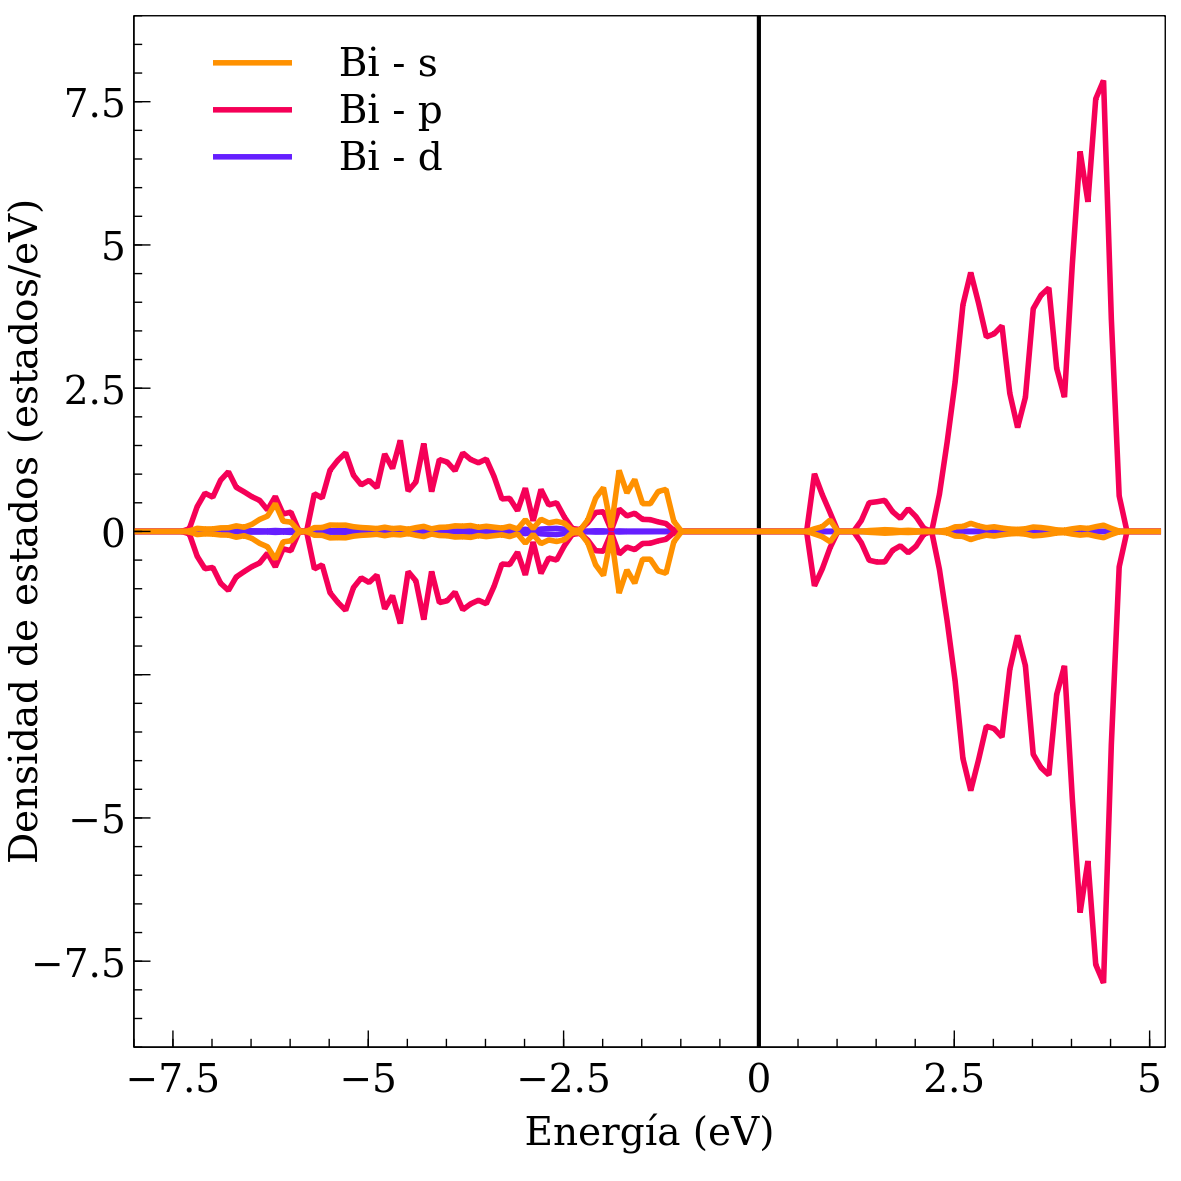
\includegraphics[width=0.5\textwidth]{contenido/resultados/ferrita_bismuto/img_ferrita_bismuto/BiFeO3_DOS_Bi_G_inf.png}}
    
    \subfloat[]{
        \label{bfo_fe_g}
        
        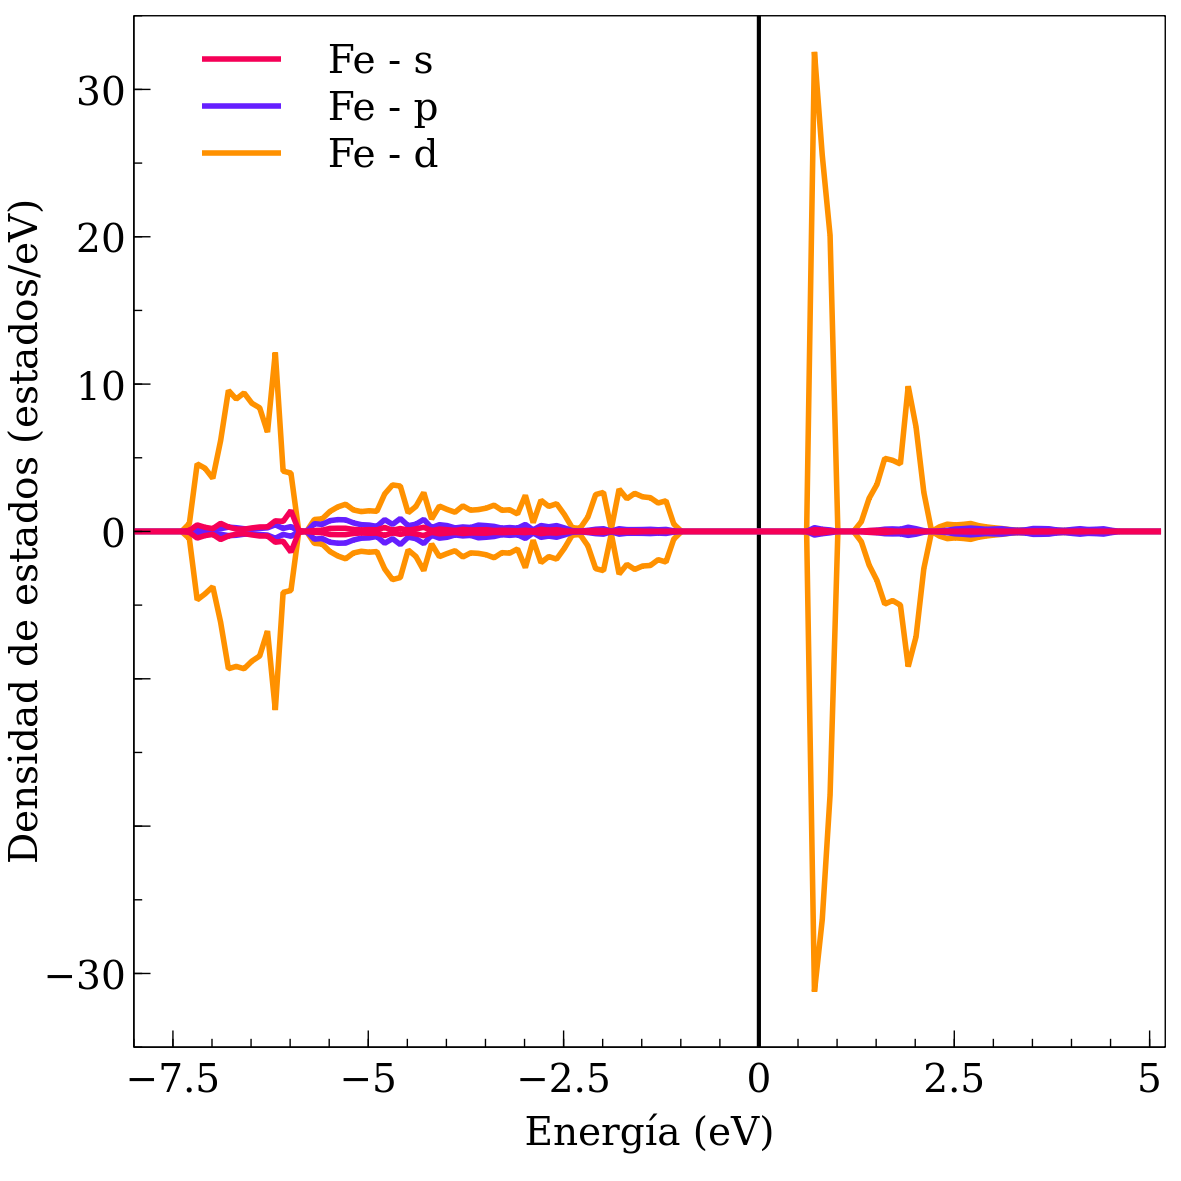
\includegraphics[width=0.5\textwidth]{contenido/resultados/ferrita_bismuto/img_ferrita_bismuto/BiFeO3_DOS_Fe_G_inf.png}}
    \subfloat[]{
        \label{bfo_o_g}
        
        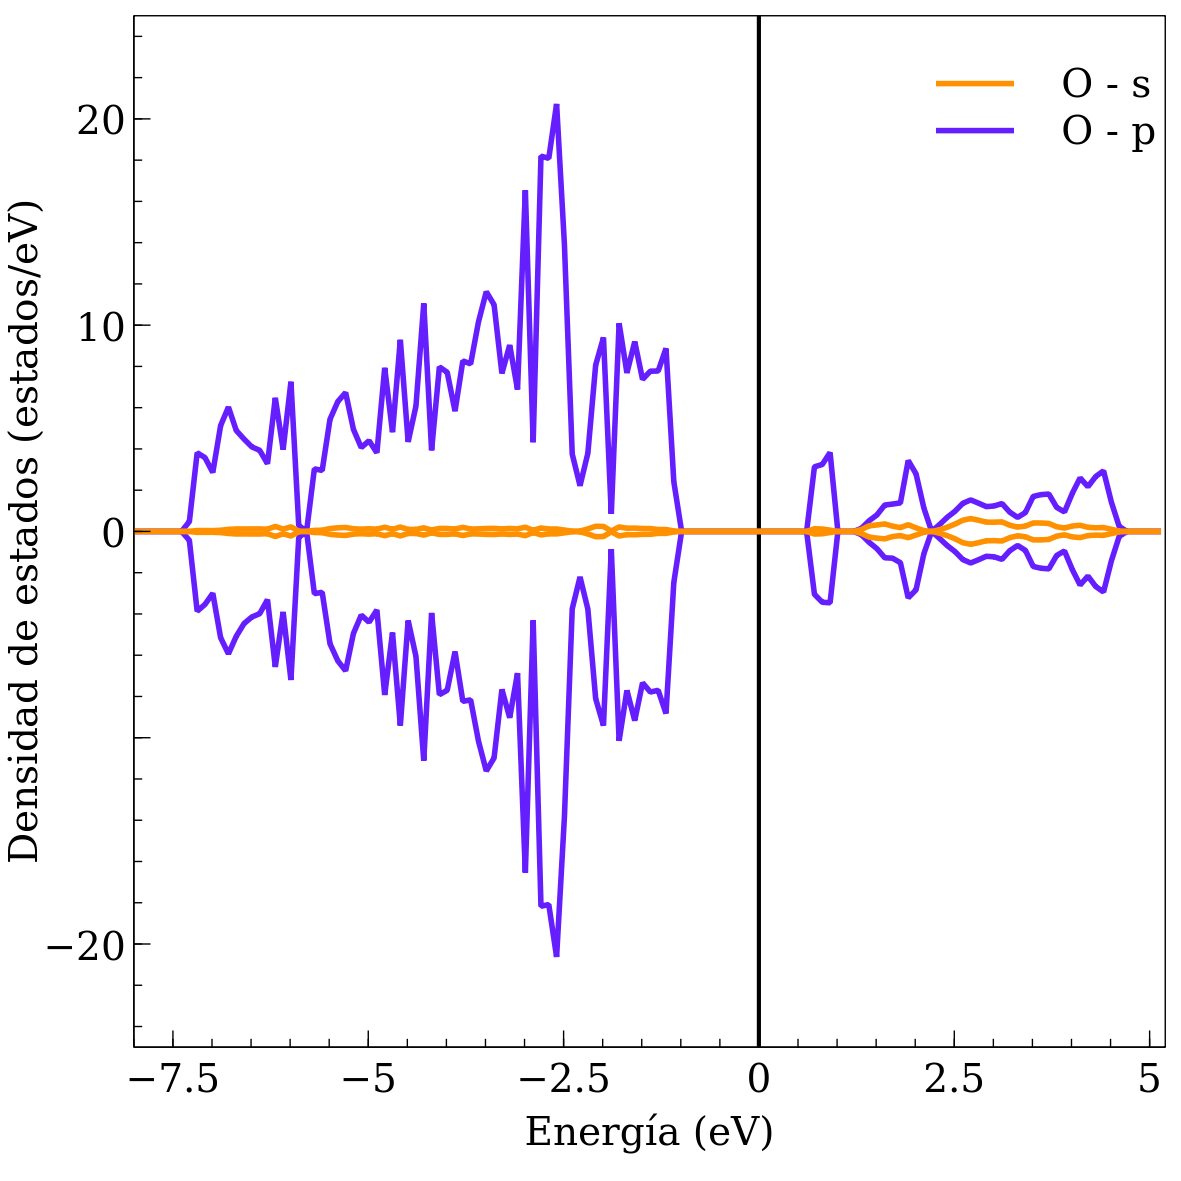
\includegraphics[width=0.5\textwidth]{contenido/resultados/ferrita_bismuto/img_ferrita_bismuto/BiFeO3_DOS_O_G_inf.png}}
    \singlespace
    \caption[Densidad de estados del $BiFeO_{3}$ con arreglo 
    antiferromagn\'etico tipo G]{Densidad de estados del $BiFeO_{3}$ 
    con 
        arreglo antiferromagn\'etico tipo G. La linea negra en cero 
        indica el 
        nivel 
        de fermi. \ref{bfo_dos_g} \subref{bfo_tot_g} Densidad de estados total 
        y de cada elemento. 
        \ref{bfo_dos_g} \subref{bfo_bi_g} 
        Densidad de 
        estados para los orbitales s, p, d del bismuto. \ref{bfo_dos_g} 
        \subref{bfo_fe_g} Densidad 
        de estados 
        para los orbitales s, p ,d del hierro. \ref{bfo_dos_g} \subref{bfo_o_g} 
        Densidad de estados 
        para los 
        orbitales s, p del ox\'igeno.}
    \label{bfo_dos_g}
\end{figure}



% -------------------------------------------------------------
% FIGURA: densidad de estado total y por elemento del BIFeO3 tipo G
% -------------------------------------------------------------

\noindent La figura \ref{bfo_dos_g} \subref{bfo_tot_g} muestra la densidad de 
estados total para 
cada elemento que compone al $BiFeO_{3}$. Las energ\'ias fueron 
escaladas respecto al 
nivel de fermi que se tomo como cero de la escala horizontal, y la 
escala 
vertical positiva y negativa corresponden a los espines up y down 
respectivamente. En la banda de conducci\'on se observa que cerca al 
nivel de fermi los estados de hierro son los predominantes con una 
densidad de aproximadamente 40 estados/eV y con una densidad m\'as 
reducida se encuentran estados de ox\'igeno seguidos de estados de 
bismuto. En el rango de $1.5$ eV a $2.5$ eV los estados de hierro 
presentan una densidad por debajo de los 20 estados/eV y los estados 
de ox\'igeno y bismuto presentan densidades similares al intervalo 
anterior. A partir del nivel de energ\'ia de $2.5$ eV los estados de 
bismuto son los predominantes con una densidad aproximada de 5 
estados/eV mezclados con estados de ox\'igeno, en este rango de 
energ\'ia el hierro presenta una densidad de estados casi nula. En la 
banda de valencia, por debajo del nivel de fermi hasta el nivel de 
energ\'ia de $-5.5$ eV el ox\'igeno posee la mayor densidad de estados, 
seguido por los estados de hierro y bismuto con una baja densidad. 
A partir del nivel de energ\'ia de $-5.5$ eV el hierro posee la mayor 
densidad de estados con aproximadamente 15 estados/eV seguido por los 
estados de ox\'igeno con una densidad similar y el bismuto posee una 
densidad casi nula en este intervalo de energ\'ia.


% -------------------------------------------------------------
% FIGURA: densidad de estado parcial bismuto del BIFeO3 tipo G
% -------------------------------------------------------------

\noindent La figura \ref{bfo_dos_g} \subref{bfo_bi_g} muestra la densidad de 
estados parcial del 
bismuto 
para cada uno de los orbitales \textbf{s}, \textbf{p} y \textbf{d}. 
Las 
energ\'ias fueron escaladas respecto al 
nivel de fermi que se tomo como cero de la escala horizontal, y la 
escala 
vertical positiva y negativa corresponden a los espines up y down 
respectivamente. En la banda de conducci\'on cerca del nivel de fermi 
hasta el nivel de energ\'ia de aproximadamente $2.5$ eV se halla una 
densidad baja de estados de bismuto, siendo el orbital \textbf{p} el 
de mayor densidad y los otros dos orbitales presentan una densidad 
casi nula. A partir de $2.5$ eV la densidad de estados del orbital 
\textbf{p} aumenta considerablemente oscilando entre 5 estados/eV y 7 
estados/eV, en contraste las densidades de estado de los orbitales 
\textbf{s} y \textbf{d} son casi nulas, por lo que no contribuyen. En 
la banda de valencia cerca del nivel de fermi hasta los $-2.5$ eV el 
orbital \textbf{s} presenta la mayor densidad seguida por la densidad 
del estado \textbf{p}, siendo la densidad del orbital \textbf{d} casi 
nula. A partir del nivel de energ\'ia $-2.5$ eV hasta los $-7.5$ eV la 
densidad del orbital \textbf{p} vuelve a ser la mayor y los dem\'as 
orbitales presentan una densidad casi nula.

% -------------------------------------------------------------
% FIGURA: densidad de estado parcial hierro del BIFeO3 tipo G
% -------------------------------------------------------------

\noindent La figura \ref{bfo_dos_g} \subref{bfo_fe_g} muestra la densidad de 
estados parcial del 
hierro para cada uno de los orbitales \textbf{s}, \textbf{p} y 
\textbf{d}. 
Las 
energ\'ias fueron escaladas respecto al 
nivel de fermi que se tomo como cero de la escala horizontal, y la 
escala 
vertical positiva y negativa corresponden a los espines up y down 
respectivamente. En la banda de conducci\'on se observa que cerca del 
nivel de fermi y hasta aproximadamente 1 eV los estados del orbital 
\textbf{d} poseen una densidad de 30 estados/eV y los otros orbitales 
presentan una densidad casi nula,  dando luego paso a un peque\~no gap 
aproximadamente en $1.5$ eV. Luego hasta el nivel de energ\'ia de 
aproximadamente $2.5$ eV el orbital \textbf{d} sigue predominando con 
una densidad de 9 estados/eV y los dem\'as orbitales contin\'uan 
presentando una densidad casi nula. En la banda de valencia hasta 
aproximadamente el nivel de energ\'ia de $-5.5$ eV la densidad de 
estados del orbital \textbf{d} predomina y los dem\'as orbitales 
presentan una densidad casi nula, a partir de los $-5.5$ eV la densidad 
del orbital \textbf{d} aumenta hasta aproximadamente 10 estados/eV y 
los dem\'as orbitales contin\'uan teniendo una densidad bastante 
peque\~na.

% -------------------------------------------------------------
% FIGURA: densidad de estado parcial oxigeno del BIFeO3 tipo G
% -------------------------------------------------------------

\noindent La figura \ref{bfo_dos_g} \subref{bfo_o_g} muestra la densidad de 
estados parcial del 
hierro para cada uno de los orbitales \textbf{s} y \textbf{p}. 
Las 
energ\'ias fueron escaladas respecto al 
nivel de fermi que se tomo como cero de la escala horizontal, y la 
escala 
vertical positiva y negativa corresponden a los espines up y down 
respectivamente. En la banda de conducci\'on se observa que el orbital 
\textbf{p} presenta la mayor densidad de estados, aproximadamente 2 
estados/eV y los orbitales \textbf{s} presentan una densidad m\'as 
reducida. En la banda de valencia se observa un comportamiento 
similar, pero el orbital \textbf{p} presenta una mayor densidad de 
estados con un m\'aximo de 30 estados/eV aproximadamente en el nivel 
de energ\'ia $-2.5$ eV en contraste la densidad de estados del orbital 
\textbf{s} es casi nula.

\subsection{Densidad de carga del $\mathbf{BiFeO_{3}}$ con arreglos      
antiferromagn\'eticos tipo A y G}

La figura \ref{bfo_DC} muestra la densidad de carga de ambos arreglos 
antiferromagn\'eticos, con el fin de poder estudiar el tipo de enlace que 
existe entre los \'atomos de hierro y ox\'igeno, debido a que se pudo observar 
en la gr\'afica de densidad de estados un mezcla entre los estados de estos 
\'atomos. La densidad de carga entre el hierro y el ox\'igeno es 
aproximadamente $0.07$ e/\AA$^{3}$ lo que indica que la interacci\'on no es 
solo i\'onica sino que puede considerarse covalente. De manera similar la 
interacci\'on entre el bismuto y el ox\'igeno no es solo i\'onica dado que 
existe una densidad de carga de $0.04$ e/\AA$^{3}$. 


% ----------------------------
% FIGURA: densidades de carga
% ----------------------------

\begin{figure}
    \centering
    \subfloat[]{
        \label{bfo_DC_A}
        
        \includegraphics[width=0.4\textwidth]{contenido/resultados/ferrita_bismuto/img_ferrita_bismuto/BiFeO3_DC_plano2_A.png}}
    \subfloat[]{
        \label{bfo_DC_G}
        
        \includegraphics[width=0.4\textwidth]{contenido/resultados/ferrita_bismuto/img_ferrita_bismuto/BiFeO3_DC_plano2_G.png}}
    \singlespace
    \caption[Densidades de carga del $BiFeO_{3}$ con arreglos 
    antiferromagn\'eticos tipo A y G]{\ref{bfo_DC} \subref{bfo_DC_A} Densidad 
    de carga del 
    arreglo 
        antiferromagn\'etico tipo A. \ref{bfo_DC} \subref{bfo_DC_G}  Densidad 
        de carga del 
        arreglo 
        antiferromagn\'etico tipo G.}
    \label{bfo_DC}
\end{figure}

% -----------------
% Cromita de itrio
% -----------------

\section{Par\'ametros estructurales, bandas de energ\'ia, densidad de estados y 
densidad de carga del $\mathbf{YCrO_{3}}$}
\subsection{Par\'ametros estructurales del $\mathbf{YCrO_{3}}$ con arreglos 
antiferromagn\'eticos tipo A, C y G}

En la tabla \ref{tabla_YCrO3_parametro_red} se recogen los par\'ametros 
estructurales (a,b,c) del $YCrO_{3}$ perteneciente al espacio de grupo Pnma, 
para los tres arreglos antiferromagn\'eticos.Los par\'ametros se obtuvieron de 
la relajaci\'on de la estructura cristalina los par\'ametros son muy cercanos a 
valores experimentales obtenidos con difracci\'on de rayos X 
\cite{remeika1956,ramesha2007}

% ------------------------------
% TABLA: parametros optimizados
% ------------------------------

\begin{table}[H]
	\begin{center}
		\begin{tabular}{cccc}
			\hline
			    & \textbf{a (\AA)} & \textbf{b (\AA)} & \textbf{c 
			(\AA)} \\
			\hline \hline
			AF-A & $5.14$ & $5.49$ & $7.41$ \\
			\hline
			AF-C & $5.15$ & $5.47$ & $7.42$ \\
			\hline
			AF-G & $5.14$ & $5.47$ & $7.41$ \\
			\hline
			\cite{remeika1956} & $5.238$ & $5.518$ & $7.54$ \\
			\hline
			\cite{ramesha2007} & $5.515$ & $5.234$ & $7.521$ \\
			\hline
		\end{tabular}
		\singlespace
		\caption[Par\'ametros de red optimizados del $YCrO_{3}$]{Comparaci\'on 
			de los par\'ametros estructurales de los tres arreglos 
			antiferromagn\'eticos, con valores obtenidos de difracci\'on de 
			rayos X.}
		\label{tabla_YCrO3_parametro_red}
	\end{center}
\end{table}

\noindent Se hall\'o que el arreglo tipo G posee el volumen m\'as peque\~no lo 
cual se 
corresponde con la energ\'ia total m\'as baja, lo cual lo hace el 
m\'as estable, 
como se muestra en la tabla \ref{tabla_YCrO3_ener_vol_mag}.

% ------------------------------------------------------------------------
% TABLA: energia total, volumen de la celda, momento magnetico del hierro
% ------------------------------------------------------------------------

 \begin{table}[H]
	\begin{center}
		\begin{tabular}{cccc}
			\hline
			\textbf{Tipo} & \textbf{Energ\'ia total (eV)} & \textbf{Volumen 
			(\AA $^{3}$)} & \textbf{Momento magn\'etico Cr ($\mu _{B}$)}\\
			\hline \hline
			AF-A & $-1462.919$ & $209.09$ & $2.75$ \\
			\hline
			AF-C & $-1462.923$ & $209.03$ & $2.70$ \\
			\hline
			AF-G & $-1462.926$ & $208.59$ & $2.65$ \\
			\hline
		\end{tabular}
		\singlespace
		\caption{Energ\'ia total, volumen de la celda y momento magn\'etico del 
		\'atomo de cromo,
			para los tres arreglos antiferromagn\'eticos}
		\label{tabla_YCrO3_ener_vol_mag}
	\end{center}
\end{table}

\noindent Los momentos magn\'eticos del cromo de los tres arreglos 
antiferromagn\'eticos 
mostrados en la tabla \ref{tabla_YCrO3_ener_vol_mag} se encuentran pr\'oximos 
al valor de 3 $\mu _{B}$, un comportamiento esperado \cite{nair2013,serrao2005}.


\subsection{Estructura de bandas de energ\'ia del $\mathbf{YCrO_{3}}$ con      
    arreglo antiferromagn\'etico tipo A}

% ----------------------------
% FIGURA: banda YCrO3 tipo A
% ----------------------------

\begin{figure}[H]
	\centering
	\includegraphics[width=0.7\textwidth]{contenido/resultados/cromita_itrio/img_cromita_itrio/YCrO3_bandas_A_inf.png}
	\singlespace
	\caption[Bandas de energ\'ia del $YCrO_{3}$ con arreglo 
	antiferromagn\'etico tipo A]{Estructura de bandas de energ\'ia del 
	$YCrO_{3}$ con arreglo antiferromagn\'etico tipo A. La linea roja marca el 
	nivel de fermi. Los puntos de alta simetr\'ia tomados en la primera zona de 
	brillouin son $\Gamma - X - S - Y - \Gamma$.}
	\label{yco_band_a}
\end{figure}


La figura \ref{yco_band_a} muestra la estructura de bandas de energ\'ia del 
$YCrO_{3}$ con arreglo antiferromagn\'etico tipo A. Las energ\'ias 
fueron escaladas 
respecto al nivel de fermi, que es tomado como el cero de la escala 
vertical. Se observa un gap de 
energ\'ia de $1.3$ eV. El 
gap se halla entre el m\'aximo de la banda de valencia y el m\'inimo de la 
banda de conducci\'on; estando ambos ubicados en el punto de alta simetr\'ia 
$\Gamma$. Por debajo del nivel de fermi en la banda de valencia 
alrededor del nivel de energ\'ia de -3 eV se observa una franja que no 
posee bandas de energ\'ia. 

\subsection{Densidad de estados del $\mathbf{YCrO_{3}}$ con arreglo      
    antiferromagn\'etico tipo A}

% -------------------------------------------
% FIGURA: densidades de estado YCrO3 tipo A
% -------------------------------------------

\begin{figure}
    \centering
    \subfloat[]{
        \label{yco_tot_a}
        \includegraphics[width=0.5\textwidth]{contenido/resultados/cromita_itrio/img_cromita_itrio/YCrO3_DOS_A_inf.png}}
    \subfloat[]{
        \label{yco_y_a}
        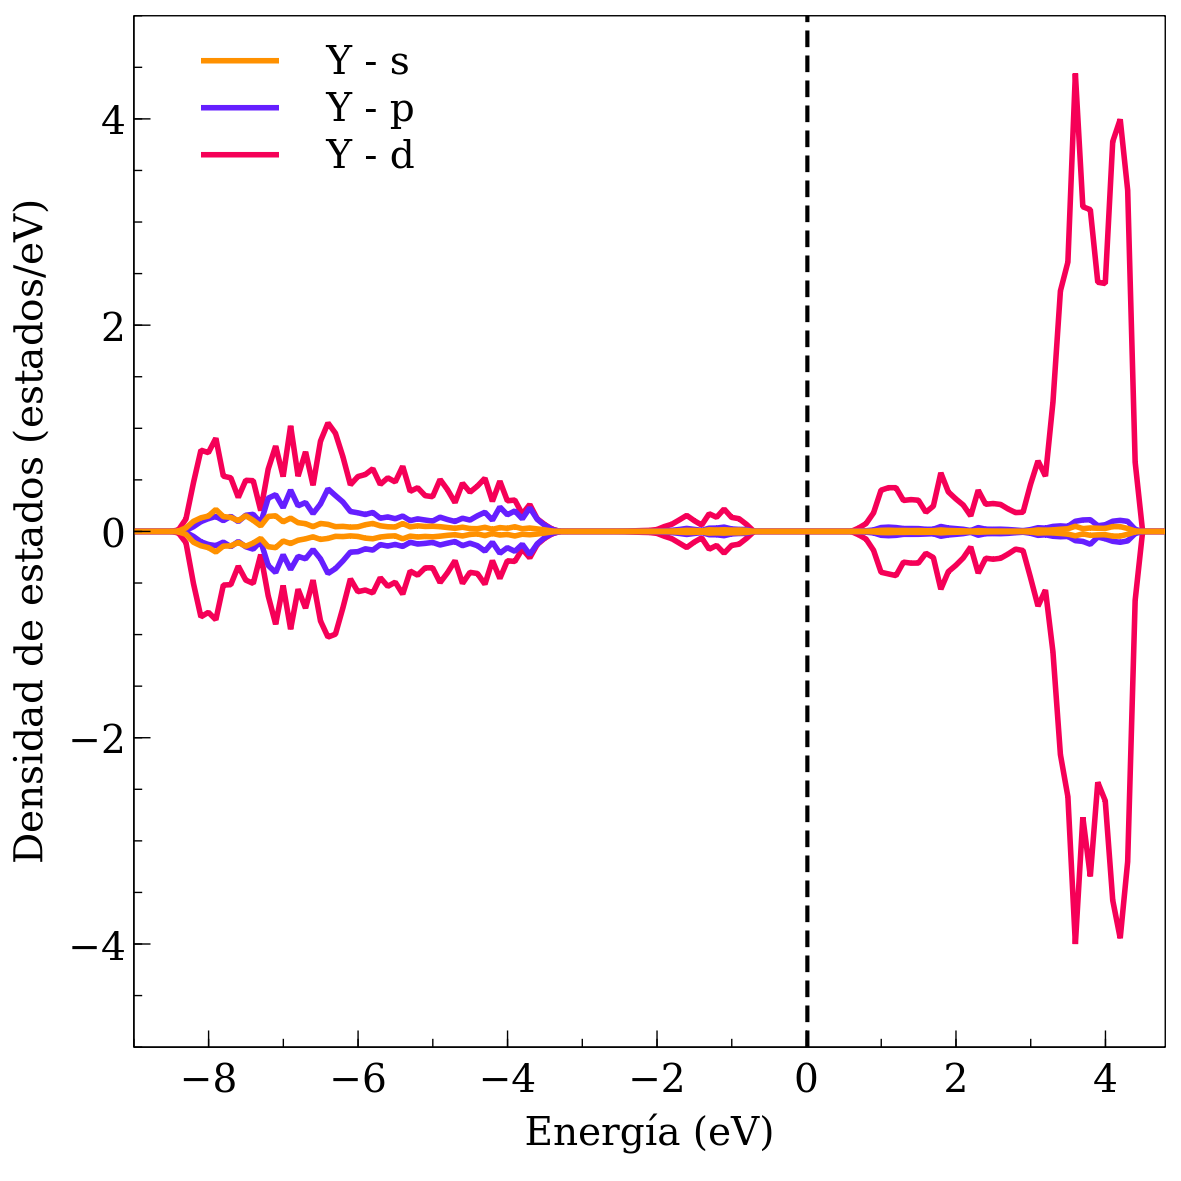
\includegraphics[width=0.5\textwidth]{contenido/resultados/cromita_itrio/img_cromita_itrio/YCrO3_DOS_Y_A_inf.png}}
    
    \subfloat[]{
        \label{yco_cr_a}
        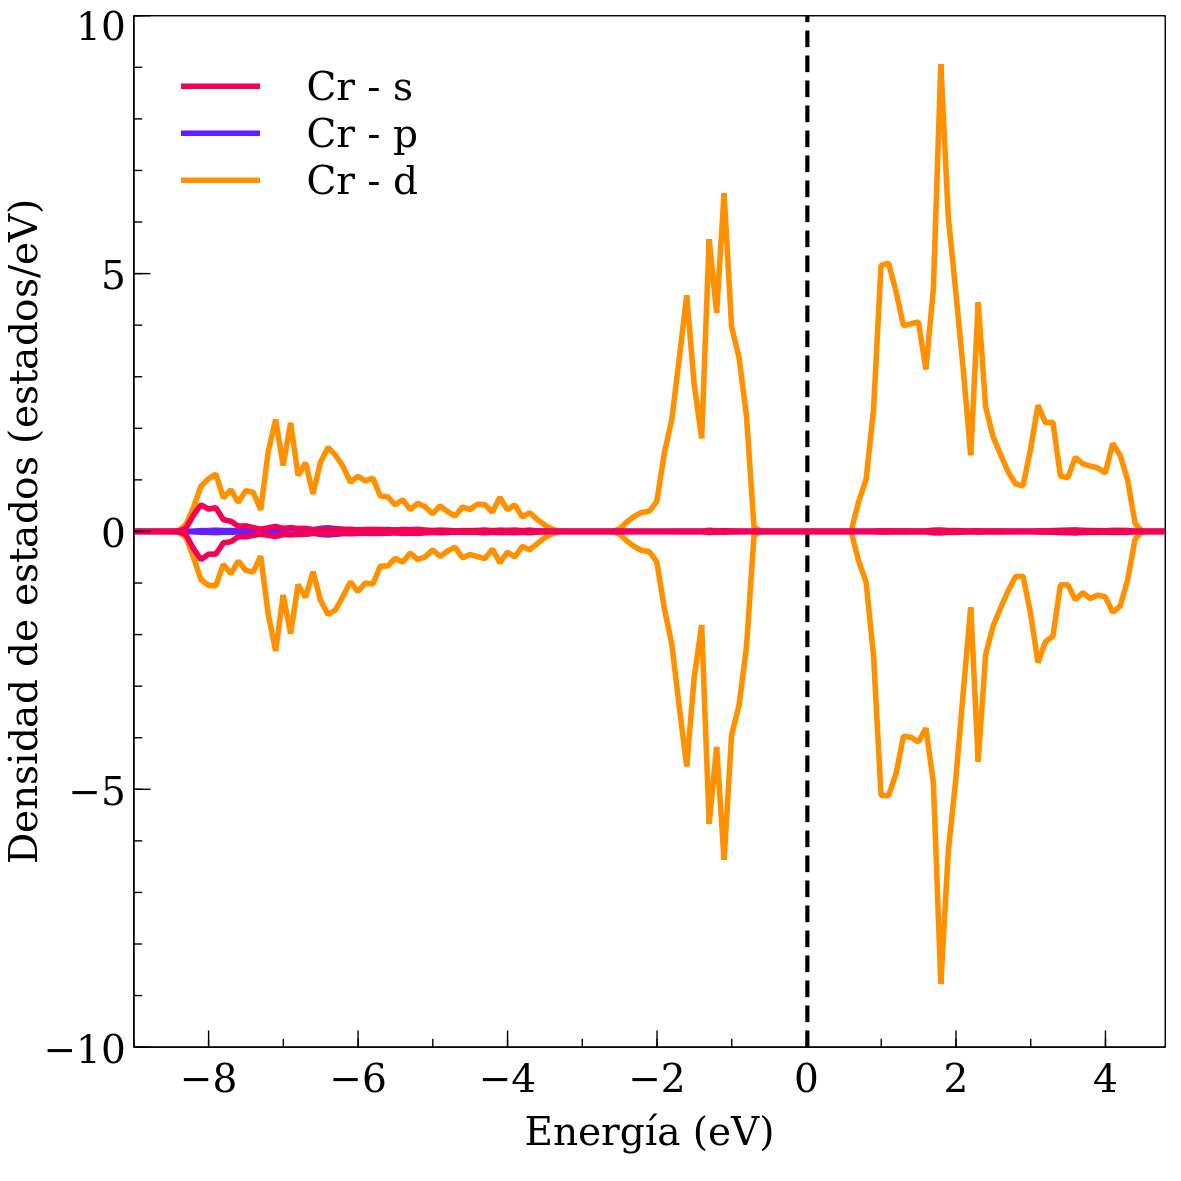
\includegraphics[width=0.5\textwidth]{contenido/resultados/cromita_itrio/img_cromita_itrio/YCrO3_DOS_Cr_A_inf.png}}
    \subfloat[]{
        \label{yco_o_a}
        \includegraphics[width=0.5\textwidth]{contenido/resultados/cromita_itrio/img_cromita_itrio/YCrO3_DOS_O_A_inf.png}}
    \singlespace
    \caption[Densidad de estados del $YCrO_{3}$ con arreglo 
    antiferromagn\'etico tipo A]{Densidad de estados del $YCrO_{3}$ 
    con arreglo 
        antiferromagn\'etico tipo A. La linea negra en cero indica el 
        nivel de 
        fermi. \ref{yco_dos_a} \subref{yco_tot_a} Densidad de estados total y 
        de cada elemento. \ref{yco_dos_a} \subref{yco_y_a} 
        Densidad de 
        estados para los orbitales s, p, d del itrio. \ref{yco_dos_a} 
        \subref{yco_cr_a} Densidad de 
        estados para 
        los orbitales s, p ,d del Cromo. \ref{yco_dos_a} \subref{yco_o_a} 
        Densidad de estados para 
        los orbitales 
        s, p del Oxigeno.}
    \label{yco_dos_a}
\end{figure}

La figura \ref{yco_dos_a} \subref{yco_tot_a} muestra la densidad de estados 
total para 
cada 
elemento que compone el $YCrO_{3}$.Las energ\'ias fueron escaladas 
respecto al 
nivel de fermi que se tomo como cero de la escala horizontal, y la 
escala 
vertical positiva y negativa corresponden a los espines up y down 
respectivamente. En la banda de conducci\'on cerca del nivel de fermi 
hasta el nivel de energ\'ia de 3 eV los estados de cromo poseen la 
mayor densidad que oscila entre 5 estados/eV y 10 estados/eV, seguido 
por la densidad de estados del ox\'igeno que es aproximadamente 2 
estados/eV y en este intervalo de energ\'ia la densidad de estados de 
itrio es muy baja. Aproximadamente a partir de los 3 eV la densidad de 
estados de itrio aumenta, alcanzando aproximadamente 4 estados/eV, 
seguido por la densidad de estados de cromo y ox\'igeno que son 
similares entre s\'i. En la banda de valencia cerca del nivel de fermi 
hasta aproximadamente -2 eV la densidad de estados de cromo es la 
mayor con aproximadamente 7 estados/eV, seguida por la densidad de 
estados de ox\'igeno con 2 estados/eV y la densidad de estados de 
itrio en este intervalo de energ\'ia es casi nula. A partir de -4 eV 
hasta -8 eV la densidad de estados de ox\'igeno es la mayor con un 
m\'aximo de 9 estados/eV, seguida por la densidad de estados de itrio 
y cromo que son similares entre s\'i con un valor de 2 estados/eV.


\noindent La figura \ref{yco_dos_a} \subref{yco_y_a} muestra la densidad de 
estados parcial del 
itrio para 
cada 
uno de los orbitales \textbf{s}, \textbf{p} y \textbf{d}.Las 
energ\'ias fueron escaladas 
respecto al 
nivel de fermi que se tomo como cero de la escala horizontal, y la 
escala 
vertical positiva y negativa corresponden a los espines up y down 
respectivamente. En la banda de conducci\'on cerca del nivel de fermi 
hasta aproximadamente 3 eV la densidad del orbital \textbf{d} es la 
mayor y las densidades de los otros orbitales son casi nulas. A partir 
de los 3 eV la densidad del orbital \textbf{d} aumenta hasta 
aproximadamente 4 estados/eV y los dem\'as orbitales mantienen una 
densidad reducida. En la banda de valencia cerca del nivel de fermi se 
observa una peque\~na densidad del orbital \textbf{d}. A partir de -4 
eV se observa un ligero aumento en las densidades de los orbitales 
\textbf{d} y \textbf{p}, pero los orbitales \textbf{s} mantienen una 
densidad casi nula.



\noindent La figura \ref{yco_dos_a} \subref{yco_cr_a} muestra la densidad de 
estados parcial del 
cromo para 
cada 
uno de los orbitales \textbf{s}, \textbf{p} y \textbf{d}.Las 
energ\'ias fueron escaladas 
respecto al 
nivel de fermi que se tomo como cero de la escala horizontal, y la 
escala 
vertical positiva y negativa corresponden a los espines up y down 
respectivamente. En la banda de conducci\'on se observa que la 
densidad del orbital \textbf{d} es la mayor en todo el rango de 
energ\'ias, con un m\'aximo de 9 estados/eV aproximadamente en 2 eV. 
En contraste los orbitales \textbf{s} y \textbf{p} no muestran una 
contribuci\'on apreciable. En la banda de valencia cerca del nivel de 
fermi hasta aproximadamente -3 eV los orbitales \textbf{d} poseen la 
mayor densidad con aproximadamente 5 estados/eV y los dem\'as 
orbitales presentan una densidad nula en este rango. En el intervalo 
de -4 eV hasta -8 eV los orbitales \textbf{d} contin\'uan siendo los 
que m\'as contribuyen y los dem\'as orbitales no muestran una 
contribuci\'on apreciable.


\noindent La figura \ref{yco_dos_a} \subref{yco_o_a} muestra la densidad de 
estados parcial del 
ox\'igeno para 
cada 
uno de los orbitales \textbf{s} y \textbf{p}.Las 
energ\'ias fueron escaladas 
respecto al 
nivel de fermi que se tomo como cero de la escala horizontal, y la 
escala 
vertical positiva y negativa corresponden a los espines up y down 
respectivamente. En la banda de conducci\'on se observa una densidad 
baja de los orbitales \textbf{p} y una densidad casi nula de orbitales 
\textbf{s}. En la banda de valencia cerca del nivel de fermi se 
observa una peque\~na densidad de orbitales \textbf{p} alrededor de -2 
eV , luego a partir de -4 eV hasta -8 eV hay un aumento considerable 
en la densidad de los orbitales \textbf{p} con un m\'aximo de 10 
estados/eV. En toda la banda de valencia la contribuci\'on de los 
orbitales \textbf{s} es muy reducida.
% ######################################################
% ######################################################

\subsection{Estructura de bandas de energ\'ia del $\mathbf{YCrO_{3}}$ con      
    arreglo antiferromagn\'etico tipo C}


% ----------------------------
% FIGURA: banda YCrO3 tipo C
% ----------------------------

\begin{figure}[H]
	\centering
	\includegraphics[width=0.7\textwidth]{contenido/resultados/cromita_itrio/img_cromita_itrio/YCrO3_bandas_C_inf.png}
	\singlespace
	\caption[Bandas de energ\'ia del $YCrO_{3}$ con arreglo 
	antiferromagn\'etico tipo C]{Estructura de bandas de energ\'ia del 
	$YCrO_{3}$ con arreglo antiferromagn\'etico tipo C. La linea roja marca el 
	nivel de fermi. Los puntos de alta simetr\'ia tomados en la primera zona de 
	brillouin son $\Gamma - X - S - Y - \Gamma$.}
	\label{yco_band_c}
\end{figure}

La figura \ref{yco_band_c} muestra la estructura de bandas de 
energ\'ia del 
$YCrO_{3}$ con arreglo antiferromagn\'etico tipo C. Las energ\'ias 
fueron escaladas 
respecto al nivel de fermi, que es tomado como el cero de la escala 
vertical. Se observa un gap de 
energ\'ia de $1.32$ eV entre el m\'inimo de la banda de conducci\'on ubicado en 
el punto $\Gamma$ y el 
m\'aximo de la banda de valencia ubicado en el punto $X$. Por debajo 
del nivel de fermi en la banda de valencia 
alrededor del nivel de energ\'ia de -3 eV se observa una franja que no 
posee bandas de energ\'ia. 

\subsection{Densidad de estados del $\mathbf{YCrO_{3}}$ con arreglo      
    antiferromagn\'etico tipo C}

% -------------------------------------------
% FIGURA: densidades de estado YCrO3 tipo C
% -------------------------------------------

\begin{figure}
    \centering
    \subfloat[]{
        \label{yco_tot_c}
        \includegraphics[width=0.5\textwidth]{contenido/resultados/cromita_itrio/img_cromita_itrio/YCrO3_DOS_C_inf.png}}
    \subfloat[]{
        \label{yco_y_c}
        \includegraphics[width=0.5\textwidth]{contenido/resultados/cromita_itrio/img_cromita_itrio/YCrO3_DOS_Y_C_inf.png}}
    
    \subfloat[]{
        \label{yco_cr_c}
        \includegraphics[width=0.5\textwidth]{contenido/resultados/cromita_itrio/img_cromita_itrio/YCrO3_DOS_Cr_C_inf.png}}
    \subfloat[]{
        \label{yco_o_c}
        \includegraphics[width=0.5\textwidth]{contenido/resultados/cromita_itrio/img_cromita_itrio/YCrO3_DOS_O_C_inf.png}}
    \singlespace
    \caption[Densidad de estados del $YCrO_{3}$ con arreglo 
    antiferromagn\'etico 
    tipo C]{Densidad de estados del $YCrO_{3}$ con arreglo 
    antiferromagn\'etico 
        tipo C. La linea negra en cero indica el nivel de fermi. 
        \ref{yco_dos_c} \subref{yco_tot_c} 
        Densidad de 
        estados total y de cada elemento. \ref{yco_dos_c} \subref{yco_y_c} 
        Densidad de estados para 
        los orbitales s, 
        p, d del itrio. \ref{yco_dos_c} \subref{yco_cr_c} Densidad de estados 
        para los orbitales s, 
        p ,d del Cromo. 
        \ref{yco_dos_c} \subref{yco_o_c} Densidad de estados para los orbitales 
        s, p del Oxigeno.}
    \label{yco_dos_c}
\end{figure}


\noindent La figura \ref{yco_dos_c} \subref{yco_tot_c} muestra la densidad de 
estados total para 
cada 
elemento que compone el $YCrO_{3}$.Las energ\'ias fueron escaladas 
respecto al 
nivel de fermi que se tomo como cero de la escala horizontal, y la 
escala 
vertical positiva y negativa corresponden a los espines up y down 
respectivamente. En la banda de conducci\'on cerca del nivel de fermi 
hasta el nivel de energ\'ia 2 eV la densidad de estados de cromo es la 
mayor con un valor de 6 estados/eV seguida por las densidades de 
ox\'igeno e itrio que son peque\~nas por debajo de 2 estados/eV. A 
partir de 3 eV la densidad de estados de itrio es la mayor con 4 
estados/eV seguida por la densidad de estados de cromo y ox\'igeno que 
son similares con aproximadamente 2 estados/eV. En la banda de 
valencia cerca del nivel de fermi hasta -2 eV la densidad de estados 
de cromo es la dominante con un valor de 7 estados/eV seguida por una 
densidad m\'as peque\~na de estados de ox\'igeno y una densidad casi 
nula de estados de itrio. A partir de -4 eV hasta -8 eV la densidad de 
estados de ox\'igeno es la mayor con un valor cercano a 10 estados/eV, 
mezclados con estados de itrio y cromo cuyas densidades de estados son 
similares con un valor de aproximadamente 2 estados/eV


\noindent La figura \ref{yco_dos_c} \subref{yco_y_c} muestra la densidad de 
estados parcial del 
itrio para 
cada 
uno de los orbitales \textbf{s}, \textbf{p} y \textbf{d}.Las 
energ\'ias fueron escaladas 
respecto al 
nivel de fermi que se tomo como cero de la escala horizontal, y la 
escala 
vertical positiva y negativa corresponden a los espines up y down 
respectivamente. En la banda de conducci\'on cerca del nivel de fermi 
hasta 2 eV se puede observar una densidad peque\~na de orbitales 
\textbf{d}, a partir de este nivel de energ\'ia aumenta la densidad de 
orbitales \textbf{d} hasta 4 estados/eV. En todo el rango de energ\'ia 
de la banda de conducci\'on la contribuci\'on de los orbitales 
\textbf{s} y \textbf{p} no es apreciable. En la banda de valencia 
cerca del nivel de fermi aproximadamente en -2
 eV se observa una peque\~na densidad de orbitales \textbf{d} y la 
 densidad de los dem\'as orbitales en ese rango es nula. A partir de 
 -4 eV hasta -8 eV aumenta un poco la densidad de orbitales \textbf{d} 
 y la densidad de orbitales \textbf{p}; la contribuci\'on de los 
 orbitales \textbf{s} sigue siendo muy peque\~na en este rango de 
 energ\'ias.
 
 
 
 \noindent La figura \ref{yco_dos_c} \subref{yco_cr_c} muestra la densidad de 
 estados parcial del 
 cromo para 
 cada 
 uno de los orbitales \textbf{s}, \textbf{p} y \textbf{d}.Las 
 energ\'ias fueron escaladas 
 respecto al 
 nivel de fermi que se tomo como cero de la escala horizontal, y la 
 escala 
 vertical positiva y negativa corresponden a los espines up y down 
 respectivamente. En la banda de valencia se observa que la densidad 
 de los orbitales \textbf{d} es la predominante en todo el rango de 
 energ\'ias con un valor de 5 estados/eV y a partir del nivel de 
 energ\'ia de 3 eV la densidad desciende por debajo de 2 estados/eV. 
 La contribuci\'on de los orbitales \textbf{s} y \textbf{p} no es 
 apreciable. En la banda de valencia cerca del nivel de fermi hasta el 
 nivel de energ\'ia de -2 eV la densidad de orbitales  \textbf{d} es 
 la mayor con un valor cercano a 10 estados/eV. A partir de -4 eV 
 hasta -8 eV la densidad de orbitales \textbf{d} desciende por debajo 
 de 2 estados/eV. Al igual que en la banda de conducci\'on los 
 orbitales \textbf{s} y \textbf{p} no contribuyen de forma apreciable.
 
 
\noindent La figura \ref{yco_dos_c} \subref{yco_o_c} muestra la densidad de 
estados parcial del 
 ox''igeno para 
 cada 
 uno de los orbitales \textbf{s} y \textbf{p}. Las 
 energ\'ias fueron escaladas 
 respecto al 
 nivel de fermi que se tomo como cero de la escala horizontal, y la 
 escala 
 vertical positiva y negativa corresponden a los espines up y down 
 respectivamente. En la banda de conducci\'on la mayor densidad 
 pertenece a los orbitales \textbf{p} pero esta es reducida, dado que 
 tiene un valor por debajo de los 2 estados/eV y la contribuci\'on del 
 orbital \textbf{s} es casi nula. En la banda de valencia cerca al 
 nivel de fermi se observa un rango peque\~no de energ\'ias con una 
 densidad de orbitales \textbf{p} reducida de aproximadamente 2 
 estados/eV. A partir de -4 eV hasta -8 eV la densidad de orbitales 
 \textbf{p} es la mayor con un rango de valores desde 3 estados/eV 
 hasta 10 estados/eV. En este rango de energ\'ias la contribuci\'on de 
 los dem\'as orbitales es casi inexistente.
 
% ######################################################
% ######################################################

\subsection{Estructura de bandas de energ\'ia del $\mathbf{YCrO_{3}}$ con      
    arreglo antiferromagn\'etico tipo G}

% ----------------------------
% FIGURA: banda YCrO3 tipo G
% ----------------------------

\begin{figure}[H]
	\centering
	\includegraphics[width=0.7\textwidth]{contenido/resultados/cromita_itrio/img_cromita_itrio/YCrO3_bandas_G_inf.png}
	\singlespace
	\caption[Bandas de energ\'ia del $YCrO_{3}$ con arreglo 
	antiferromagn\'etico tipo G]{Estructura de bandas de energ\'ia del 
	$YCrO_{3}$ con arreglo antiferromagn\'etico tipo G. La l\'inea roja marca 
	el 
	nivel de fermi. Los puntos de alta simetr\'ia tomados en la primera zona de 
	brillouin son $\Gamma - X - S - Y - \Gamma$.}
	\label{yco_band_g}
\end{figure}


La figura \ref{yco_band_g} muestra la estructura de bandas de energ\'ia del 
$YCrO_{3}$ con arreglo antiferromagn\'etico tipo G.  Las energ\'ias 
fueron escaladas 
respecto al nivel de fermi, que es tomado como el cero de la escala 
vertical.Se observa un gap de 
energ\'ia de $1.6$ eV el cual es cercano al valor de $1.64$ reportado por otro 
estudio \cite{nair2013}. El gap esta definido entre el m\'inimo de la banda de 
conducci\'on ubicado en el punto $S$ 
y el m\'aximo de la banda de conducci\'on ubicado en el punto 
$\Gamma$. Por debajo 
del nivel de fermi en la banda de valencia 
alrededor del nivel de energ\'ia de -3 eV se observa una franja que no 
posee bandas de energ\'ia. Por sobre el nivel de fermi alrededor de 3 
eV se halla una regi\'on que no posee bandas de energ\'ia.


\subsection{Densidad de estados del $\mathbf{YCrO_{3}}$ con arreglo      
    antiferromagn\'etico tipo G}

% -------------------------------------------
% FIGURA: densidades de estado YCrO3 tipo G
% -------------------------------------------

\begin{figure}[H]
    \centering
    \subfloat[]{
        \label{yco_tot_g}
        \includegraphics[width=0.5\textwidth]{contenido/resultados/cromita_itrio/img_cromita_itrio/YCrO3_DOS_G_inf.png}}
    \subfloat[]{
        \label{yco_y_g}
        \includegraphics[width=0.5\textwidth]{contenido/resultados/cromita_itrio/img_cromita_itrio/YCrO3_DOS_Y_G_inf.png}}
    
    \subfloat[]{
        \label{yco_cr_g}
        \includegraphics[width=0.5\textwidth]{contenido/resultados/cromita_itrio/img_cromita_itrio/YCrO3_DOS_Cr_G_inf.png}}
    \subfloat[]{
        \label{yco_o_g}
        \includegraphics[width=0.5\textwidth]{contenido/resultados/cromita_itrio/img_cromita_itrio/YCrO3_DOS_O_G_inf.png}}
    \singlespace
    \caption[Densidad de estados del $YCrO_{3}$ con arreglo 
    antiferromagn\'etico 
    tipo G]{Densidad de estados del $YCrO_{3}$ con arreglo 
    antiferromagn\'etico 
        tipo G. La linea negra en cero indica el nivel de fermi. 
        \ref{yco_dos_g} \subref{yco_tot_g} 
        Densidad de 
        estados total y de cada elemento. \ref{yco_dos_g} \subref{yco_y_g} 
        Densidad de estados para 
        los orbitales s, 
        p, d del itrio. \ref{yco_dos_g} \subref{yco_cr_g} Densidad de estados 
        para los orbitales s, 
        p ,d del Cromo. 
        \ref{yco_dos_g} \subref{yco_o_g} Densidad de estados para los orbitales 
        s, p del Oxigeno.}
    \label{yco_dos_g}
\end{figure}


La figura \ref{yco_dos_g} \subref{yco_tot_g} muestra la densidad de estados 
total para 
cada 
elemento que compone el $YCrO_{3}$.Las energ\'ias fueron escaladas 
respecto al 
nivel de fermi que se tomo como cero de la escala horizontal, y la 
escala 
vertical positiva y negativa corresponden a los espines up y down 
respectivamente. En la banda de conducci\'on cerca del nivel de fermi 
hasta aproximadamente 2 eV se observa que la densidad de estados del 
cromo es la mayor con un m\'aximo de 10 estados/eV en ese rango de 
energ\'ias las densidades de estado del itrio y del ox\'igeno son 
reducidas con valores por debajo de 2 estados/eV. Alrededor de 3 eV se 
observa una zona que no esta ocupada por ning\'un estado. A partir de 
aproximadamente $3.5$ eV la mayor densidad pertenece al itrio con un 
valor de 4 estados/eV, tambi\'en se encuentran las densidades de cromo 
y ox\'igeno que son similares entre s\'i con un valor menor a 2 
estados/eV. En la banda de valencia cerca del nivel de fermi hasta 
aproximadamente -2 eV la mayor densidad pertenece al cromo con un 
valor de 6 estados/eV, tambi\'en se encuentran estados de ox\'igeno e 
itrio por debajo de los 2 estados/eV. En el rango de -4 eV hasta -8 eV 
el ox\'igeno posee la mayor densidad de estados con valores de entre 4 
estados/eV hasta 10 estados/eV, tambi\'en se encuentran estados de 
cromo e itrio cuyas densidades son similares con un valor por debajo 
de 3 estados/eV.


\noindent La figura \ref{yco_dos_g} \subref{yco_y_g} muestra la densidad de 
estados parcial del 
itrio para 
cada 
uno de los orbitales \textbf{s}, \textbf{p} y \textbf{d}.Las 
energ\'ias fueron escaladas 
respecto al 
nivel de fermi que se tomo como cero de la escala horizontal, y la 
escala 
vertical positiva y negativa corresponden a los espines up y down 
respectivamente. En la banda de conducci\'on cerca del nivel de fermi 
hasta aproximadamente $2.5$ eV se observa una peque\~na densidad de 
orbitales \textbf{d} con un valor de 1 estado/eV. Luego a partir de 3 
eV la densidad de orbitales \textbf{d} aumenta hasta 4 estados/eV. En 
todo el rango de energ\'ias de la banda de conducci\'on las 
contribuciones de los orbitales \textbf{s} y \textbf{p} no son 
apreciables. En la banda de valencia se observa una densidad de 
orbitales \textbf{d} peque\~na cerca del nivel de fermi. A partir de 
-4 eV hasta -8 eV la densidad de orbitales \textbf{d} es la mayor y  
se encuentra por debajo de 2 estados/eV, y en este rango los orbitales 
\textbf{s} y \textbf{p} tienen una densidad similar y bastante 
peque\~na.



\noindent La figura \ref{yco_dos_g} \subref{yco_cr_g} muestra la densidad de 
estados parcial del 
cromo para 
cada 
uno de los orbitales \textbf{s}, \textbf{p} y \textbf{d}.Las 
energ\'ias fueron escaladas 
respecto al 
nivel de fermi que se tomo como cero de la escala horizontal, y la 
escala 
vertical positiva y negativa corresponden a los espines up y down 
respectivamente. En la banda de conducci\'on se observa que los 
orbitales \textbf{d} tienen la mayor densidad en todo el rango de 
energ\'ias. Con valores de densidad de 10 estados/eV cerca del nivel 
de fermi hasta aproximadamente 2 eV. Luego la densidad se reduce por 
debajo de 3 estados/eV a partir del nivel de energ\'ia de 3 eV. Las 
contribuciones de los dem\'as orbitales son nulas en la banda de 
conducci\'on. En la banda de valencia cerca al nivel de fermi hasta -2 
eV se tiene una densidad de orbitales \textbf{d} con un valor 
aproximado de 6 estados/eV. Luego a partir de -4 eV hasta -8 eV la 
densidad se reduce por debajo de 3 estados/eV pero siguen predominando 
los orbitales \textbf{d}. En la banda de valencia tampoco existe una 
contribuci\'on apreciable de los orbitales \textbf{s} y \textbf{p}.


\noindent La figura \ref{yco_dos_g} \subref{yco_o_g} muestra la densidad de 
estados parcial del 
ox\'igeno para 
cada 
uno de los orbitales \textbf{s} y \textbf{p}.Las 
energ\'ias fueron escaladas 
respecto al 
nivel de fermi que se tomo como cero de la escala horizontal, y la 
escala 
vertical positiva y negativa corresponden a los espines up y down 
respectivamente. En la banda de conducci\'on cerca del nivel de fermi 
hasta aproximadamente 2 eV se observa una peque\~na densidad del 
orbital \textbf{p} con un valor por debajo de 3 estados/eV. Y 
alrededor de 4 eV tambi\'en se halla una densidad de los orbitales 
\textbf{p} peque\~na por debajo de 2 estados/eV. Adem\'as la 
contribuci\'on del orbital \textbf{s} en la banda de conducci\'on es 
reducida. En la banda de valencia cerca al nivel de fermi se observa 
una densidad peque\~na del orbital \textbf{p} por debajo de 2 
estados/eV. En el rango de -4 eV hasta -8 eV los orbitales \textbf{p} 
tienen la mayor densidad con valores entre 4 estados/eV hasta 10 
estados/eV. En la banda de valencia la contribuci\'on del orbital 
\textbf{s} no es significativa.

% ######################################################
% ######################################################

\subsection{Densidad de carga del $\mathbf{YCrO_{3}}$ con arreglos      
    antiferromagn\'eticos tipo A, C y G}

% ----------------------------
% FIGURA: densidades de carga
% ----------------------------

\begin{figure}[H]
	\centering
	\subfloat[]{
		\label{yco_DC_A}
		\includegraphics[width=0.33\textwidth]{contenido/resultados/cromita_itrio/img_cromita_itrio/YCrO3_DC_plano2_A.png}}
	\subfloat[]{
		\label{yco_DC_C}
		\includegraphics[width=0.33\textwidth]{contenido/resultados/cromita_itrio/img_cromita_itrio/YCrO3_DC_plano2_C.png}}
	\subfloat[]{
		\label{yco_DC_G}
		\includegraphics[width=0.33\textwidth]{contenido/resultados/cromita_itrio/img_cromita_itrio/YCrO3_DC_plano2_G.png}}
	\singlespace
	\caption[Densidades de carga del $YCrO_{3}$ con arreglos 
	antiferromagn\'eticos tipo A,C y G]{\ref{yco_DC} \subref{yco_DC_A} Densidad 
	de carga del arreglo 
	antiferromagn\'etico tipo A. \ref{yco_DC} \subref{yco_DC_C}  Densidad de 
	carga del arreglo 
	antiferromagn\'etico tipo C. \ref{yco_DC} \subref{yco_DC_G}  Densidad de 
	carga del arreglo 
	antiferromagn\'etico tipo G.}
	\label{yco_DC}
\end{figure}

La figura \ref{yco_DC} muestra la densidad de carga de los tres arreglos 
antiferromagn\'eticos, con el fin de poder estudiar el tipo de enlace que 
existe entre los \'atomos de cromo y ox\'igeno, debido a que se pudo observar 
en la gr\'afica de densidad de estados un mezcla entre los estados de estos 
\'atomos. La densidad de carga entre el cromo y el ox\'igeno es 
aproximadamente $0.3$ e/\AA$^{3}$ lo que indica que la interacci\'on no es 
solo i\'onica sino que puede considerarse covalente. De manera similar la 
interacci\'on entre el itrio y el ox\'igeno se asocia con una densidad de carga 
de $0.02$ e/\AA$^{3}$.



    
    % -----------------------
    % Conclusiones
    % -----------------------
    
    \chapter*{Conclusiones}
    \addcontentsline{toc}{chapter}{Conclusiones}
    Para el $BiFeO_{3}$ se observ\'o un gap de energ\'ia de $1.4$ eV y $1.8$ eV 
para los arreglos antiferromagn\'eticos tipo A y G respectivamente. Adem\'as  
el comportamiento de ambos arreglos 
antiferromagn\'eticos es similar, esto se puede atribuir a que los orbitales 
\textbf{d} del hierro 
son los que poseen la mayor densidad cerca del nivel de fermi en la banda de 
conducci\'on y en la banda de valencia cerca del nivel de fermi son los 
orbitales \textbf{p} del ox\'igeno los que poseen la mayor densidad. Adem\'as 
en ambos arreglos antiferromagn\'eticos se observa que los estados de los tres 
elementos se encuentran mezclados a lo largo de todo el rango de energ\'ias. De 
los resultados obtenidos se concluy\'o que el arreglo antiferromagn\'etico tipo 
C para el $BiFeO_{3}$ no converge.


\noindent En el caso del $YCrO_{3}$ se observ\'o un gap de energ\'ia de $1.3$ 
eV, $1.32$ eV y $1.6$ eV 
para los arreglos antiferromagn\'eticos tipo A, C y G respectivamente. Adem\'as 
los tres arreglos antiferromagn\'eticos presentan un comportamiento similar, 
esto se puede atribuir a que 
los orbitales \textbf{d} del cromo son los que poseen la mayor densidad de 
estados cerca del nivel de fermi tanto en la banda de valencia como en la banda 
de conducci\'on. Tambi\'en se observa que los estados de los tres elementos se 
encuentran mezclados a lo largo de todo el rango de energ\'ias.
En el caso de arreglo antiferromagn\'etico tipo G del $YCrO_{3}$ se observ\'o 
que presenta un segundo gap por sobre el nivel de fermi, una caracter\'istica 
que no se encuentra presente en los otros dos tipos de arreglos 
antiferromagn\'eticos.

\noindent Los resultados obtenidos pueden considerarse como punto de partida 
para futuras investigaciones en las cuales se pueden introducir nuevos 
par\'ametros como la temperatura, es decir simular fases tanto del $BiFeO_{3}$ 
como del $YCrO_{3}$ que se presenten a temperaturas m\'as altas. Adem\'as es 
posible estudiar la variaci\'on de la magnetizaci\'on en ambos materiales 
haciendo uso del m\'etodo monte carlo.
    
     % -----------------------
     % Apendice
     % -----------------------
     
     \appendix
     % ==========================
% PROGRAMAS AUXILIARES
% ==========================

\chapter{Scripts de entrada de Quantum ESPRESSO}
La suite Quantum ESPRESSO utiliza archivos de entrada con formato de texto plano que controlan varios aspectos de la simulaci\'on. A continuaci\'on se muestran los archivos de entrada para cada uno de los pasos realizados en el presente trabajo y partes relevantes de los archivos de salida obtenidos. Se tomara como ejemplo el caso del $YCrO_{3}$.

\noindent El primer paso es realizar un c\'alculo autoconsistente para lo cual el archivo de entrada es el siguiente.

\lstset{breaklines=true}
\begin{lstlisting}
&CONTROL
    calculation = "scf"
    max_seconds =  8.64000e+04
    pseudo_dir  = "/home/ngt/.burai/.pseudopot"
    verbosity = "high"
    restart_mode= "from_scratch"
    outdir = "./"
    prefix = "YCrO3"
/
&SYSTEM
    degauss                   =  0.01
    ecutrho                   =  320.0
    ecutwfc                   =  40.0
    hubbard_u(3)              =  1.13
    hubbard_u(4)              =  1.13
    ibrav                     = 0
    lda_plus_u                = .TRUE.
    nat                       = 20
    nspin                     = 2
    ntyp                      = 4
    nbnd                      = 200
    occupations               = "smearing"
    smearing                  = "gaussian"
    starting_magnetization(1) =  0.00000e+00
    starting_magnetization(2) =  0.00000e+00
    starting_magnetization(3) = -0.8
    starting_magnetization(4) = 0.8
/
&ELECTRONS
    conv_thr         =  1.00000e-06
    diagonalization  = "cg"
    electron_maxstep = 200
    mixing_beta      =  4.00000e-01
    mixing_mode      = "plain"
    startingpot      = "atomic"
    startingwfc      = "atomic+random"
/
K_POINTS {automatic}
6 5 6 0 0 0
CELL_PARAMETERS (angstrom)
    4.996000218   0.000000000  -0.000000233
    0.000000000   5.336857594   0.000000000
   -0.000000393   0.000000000   7.222627972
ATOMIC_SPECIES
Y      88.90585  y_lda_v1.4.uspp.F.UPF
O      15.99940  o_lda_v1.2.uspp.F.UPF
Cr2    51.99610  cr_lda_v1.5.uspp.F.UPF
Cr1    51.99610  cr_lda_v1.5.uspp.F.UPF
ATOMIC_POSITIONS (crystal)
Y        0.020236872   0.926655434   0.750000060
Y        0.520236872   0.573343566   0.250000060
Y        0.479762128   0.426656434   0.749999940
Y        0.979763128   0.073343566   0.249999940
Cr1     -0.000000000   0.500000000   0.500000000
Cr2      0.500000000   0.000000000   0.500000000
Cr1      0.500000000   0.000000000  -0.000000000
Cr2      0.000000000   0.500000000   0.000000000
O        0.688186536   0.303519361   0.448766518
O        0.188186682   0.196480479   0.551233470
O        0.811813464   0.803519361   0.051233482
O        0.311813318   0.696480479   0.948766530
O        0.311813464   0.696480639   0.551233482
O        0.811813318   0.803519521   0.448766530
O        0.188186536   0.196480639   0.948766518
O        0.688186682   0.303519521   0.051233470
O        0.103419514   0.472184554   0.250000004
O        0.603419514   0.027815446   0.750000004
O        0.396580486   0.972183554   0.249999996
O        0.896580486   0.527815446   0.749999996
\end{lstlisting}

\noindent Para iniciar la simulaci\'on se debe ejecutar el programa \textbf{pw.x} y pasarle como par\'ametro el nombre del archivo de entrada y un nombre para el archivo de salida. Como se muestra a continuaci\'on

\begin{lstlisting}
pw.x < YCrO3.scf.in > YCrO3.scf.out
\end{lstlisting}

\noindent El archivo de salida es extenso ya que contiene todas las iteraciones realizadas hasta alcanzar la convergencia. A continuaci\'on se muestra la parte del archivo donde se indica la energ\'ia de fermi y la energ\'ia total del sistema que se obtienen al converger.

\begin{lstlisting}
     the Fermi energy is    15.8431 ev

!    total energy              =   -1462.92649544 Ry
     Harris-Foulkes estimate   =   -1462.92649533 Ry
     estimated scf accuracy    <       0.00000044 Ry

     The total energy is the sum of the following terms:

     one-electron contribution =    -390.25792036 Ry
     hartree contribution      =     309.61691899 Ry
     xc contribution           =    -287.64822073 Ry
     ewald contribution        =   -1094.88316284 Ry
     Hubbard energy            =       0.24588950 Ry
     smearing contrib. (-TS)   =      -0.00000000 Ry

     total magnetization       =     0.00 Bohr mag/cell
     absolute magnetization    =    11.08 Bohr mag/cell

     convergence has been achieved in  10 iterations
\end{lstlisting}

\noindent A continuaci\'on se calcula la densidad de carga para lo cual el archivo de entrada es el siguiente.

\begin{lstlisting}
&inputpp
prefix="YCrO3"
outdir="./"
filplot="YCrO3.rho.dat"
plot_num=0
/
&plot
nfile=1
filepp(1)="YCrO3.rho.dat"
weight(1)=1.0
iflag=3
output_format=3
nx=50
ny=50
nz=50
fileout="YCrO3.plot.rho.xsf"
/
\end{lstlisting}

\noindent El anterior archivo de entrada debe ser pasado como par\'ametro al programa \textbf{pp.x}. El archivo de salida obtenido \textbf{YCrO3.rho.dat} posee un formato que esta dise\~nado para ser le\'ido por \textbf{pp.x} que sirve para realizar un segundo procesamiento y obtener el archivo \textbf{YCrO3.plot.rho.xsf} que posee un formato dise\~nado para ser le\'ido por el programa Xcrysden el cual es usado para graficar la densidad de carga.

\begin{lstlisting}
pp.x < YCrO3.rho.in > YCrO3.rho.out
\end{lstlisting}

\noindent El siguiente paso es calcular la densidad de estados para lo cual el archivo de entrada es el siguiente.

\begin{lstlisting}
&CONTROL
    calculation = "nscf"
    max_seconds =  8.64000e+04
    pseudo_dir  = "/home/ngt/.burai/.pseudopot"
    verbosity = "high"
    restart_mode= "from_scratch"
    outdir = "./"
    prefix = "YCrO3"
/
&SYSTEM
    degauss                   =  0.01
    ecutrho                   =  320.0
    ecutwfc                   =  40.0
    hubbard_u(3)              =  1.13
    hubbard_u(4)              =  1.13
    ibrav                     = 0
    lda_plus_u                = .TRUE.
    nat                       = 20
    nspin                     = 2
    ntyp                      = 4
    nbnd                      = 200
    occupations               = "tetrahedra"
    smearing                  = "gaussian"
    starting_magnetization(1) =  0.00000e+00
    starting_magnetization(2) =  0.00000e+00
    starting_magnetization(3) = -0.8
    starting_magnetization(4) = 0.8
/
&ELECTRONS
    conv_thr         =  1.00000e-06
    diagonalization  = "cg"
    electron_maxstep = 200
    mixing_beta      =  4.00000e-01
    mixing_mode      = "plain"
    startingpot      = "atomic"
    startingwfc      = "atomic+random"
/
K_POINTS {automatic}
8 7 8 0 0 0
CELL_PARAMETERS (angstrom)
    4.996000218   0.000000000  -0.000000233
    0.000000000   5.336857594   0.000000000
   -0.000000393   0.000000000   7.222627972
ATOMIC_SPECIES
Y      88.90585  y_lda_v1.4.uspp.F.UPF
O      15.99940  o_lda_v1.2.uspp.F.UPF
Cr2    51.99610  cr_lda_v1.5.uspp.F.UPF
Cr1    51.99610  cr_lda_v1.5.uspp.F.UPF
ATOMIC_POSITIONS (crystal)
Y        0.020236872   0.926655434   0.750000060
Y        0.520236872   0.573343566   0.250000060
Y        0.479762128   0.426656434   0.749999940
Y        0.979763128   0.073343566   0.249999940
Cr1     -0.000000000   0.500000000   0.500000000
Cr2      0.500000000   0.000000000   0.500000000
Cr1      0.500000000   0.000000000  -0.000000000
Cr2      0.000000000   0.500000000   0.000000000
O        0.688186536   0.303519361   0.448766518
O        0.188186682   0.196480479   0.551233470
O        0.811813464   0.803519361   0.051233482
O        0.311813318   0.696480479   0.948766530
O        0.311813464   0.696480639   0.551233482
O        0.811813318   0.803519521   0.448766530
O        0.188186536   0.196480639   0.948766518
O        0.688186682   0.303519521   0.051233470
O        0.103419514   0.472184554   0.250000004
O        0.603419514   0.027815446   0.750000004
O        0.396580486   0.972183554   0.249999996
O        0.896580486   0.527815446   0.749999996
\end{lstlisting}

\noindent Este archivo debe ser pasado como par\'ametro del programa \textbf{pw.x} e indicando un archivo de salida.

\begin{lstlisting}
pw.x < YCrO3.nscf.in > YCrO3.nscf.out
\end{lstlisting}

\noindent A continuaci\'on para poder extraer la informaci\'on correspondiente a la densidad de estados total y parcial de cada elemento se debe usar el programa \textbf{projwfc.x} con el siguiente archivo de entrada.

\begin{lstlisting}
&PROJWFC
prefix="YCrO3"
outdir="./"
ngauss=0
degauss=0.01
Emin=-40
Emax=32
DeltaE=0.1
filpdos="YCrO3.dos-proyec"
filproj="YCrO3.proyeccion.dos"
/
\end{lstlisting}

\noindent Luego ejecutamos \textbf{projwfc.x}

\begin{lstlisting}
projwfc.x < YCrO3.dos.proyeccion.in > YCrO3.dos.proyeccion.out
\end{lstlisting}

\noindent Los archivos resultantes de este paso son luego procesados por el programa escrito en python suma\_pdos.py para realizar las gr\'aficas de densidad de estados. Se cre\'o un script de shell que automatiza la ejecuci\'on del programa suma\_pdos.py, este script se encuentra en el ap\'endice de programas auxiliares.

\noindent El siguiente paso es calcular la estructura de bandas para lo cual el archivo de entrada es el siguiente.

\begin{lstlisting}
&CONTROL
    calculation = "bands"
    max_seconds =  8.64000e+04
    pseudo_dir  = "/home/ngt/.burai/.pseudopot"
    verbosity = "high"
    restart_mode= "from_scratch"
    outdir = "./"
    prefix = "YCrO3"
/
&SYSTEM
    ibrav                     = 8
    a                         =  4.996000218
    b                         =  5.336857594
    c                         =  7.222627972
    degauss                   =  0.01
    ecutrho                   =  320.0
    ecutwfc                   =  40.0
    hubbard_u(3)              =  1.13
    hubbard_u(4)              =  1.13
    lda_plus_u                = .TRUE.
    nat                       = 20
    nspin                     = 2
    ntyp                      = 4
    nbnd                      = 200
    occupations               = "smearing"
    smearing                  = "gaussian"
    starting_magnetization(1) =  0.00000e+00
    starting_magnetization(2) =  0.00000e+00
    starting_magnetization(3) = -0.8
    starting_magnetization(4) = 0.8
/
&ELECTRONS
    conv_thr         =  1.00000e-06
    diagonalization  = "cg"
    electron_maxstep = 200
    mixing_beta      =  4.00000e-01
    mixing_mode      = "plain"
    startingpot      = "atomic"
    startingwfc      = "atomic+random"
/
K_POINTS {tpiba_b}
5
gG     20
X      20
S      20
Y      20
gG     0
ATOMIC_SPECIES
Y      88.90585  y_lda_v1.4.uspp.F.UPF
O      15.99940  o_lda_v1.2.uspp.F.UPF
Cr2    51.99610  cr_lda_v1.5.uspp.F.UPF
Cr1    51.99610  cr_lda_v1.5.uspp.F.UPF
ATOMIC_POSITIONS (crystal)
Y        0.020236872   0.926655434   0.750000060
Y        0.520236872   0.573343566   0.250000060
Y        0.479762128   0.426656434   0.749999940
Y        0.979763128   0.073343566   0.249999940
Cr1     -0.000000000   0.500000000   0.500000000
Cr2      0.500000000   0.000000000   0.500000000
Cr1      0.500000000   0.000000000  -0.000000000
Cr2      0.000000000   0.500000000   0.000000000
O        0.688186536   0.303519361   0.448766518
O        0.188186682   0.196480479   0.551233470
O        0.811813464   0.803519361   0.051233482
O        0.311813318   0.696480479   0.948766530
O        0.311813464   0.696480639   0.551233482
O        0.811813318   0.803519521   0.448766530
O        0.188186536   0.196480639   0.948766518
O        0.688186682   0.303519521   0.051233470
O        0.103419514   0.472184554   0.250000004
O        0.603419514   0.027815446   0.750000004
O        0.396580486   0.972183554   0.249999996
O        0.896580486   0.527815446   0.749999996
\end{lstlisting}

\noindent El archivo anterior debe ser pasado como par\'ametro del programa \textbf{pw.x} del siguiente modo.

\begin{lstlisting}
pw.x < YCrO3.bandas.in > YCrO3.bandas.out
\end{lstlisting}

\noindent A continuaci\'on para extraer la informaci\'on de las bandas se utiliza el programa \textbf{bands.x} con el siguiente archivo de entrada.

\begin{lstlisting}
&BANDS
prefix="YCrO3"
outdir="./"
filband="YCrO3.bandas.general"
/
\end{lstlisting}

\noindent Luego ejecutamos \textbf{bands.x}.

\begin{lstlisting}
bands.x < YCrO3.ext-band-gen.in > YCrO3.ext-band-gen.out
\end{lstlisting}

\noindent El paso anterior es el \'ultimo en el proceso de simulaci\'on.

\chapter{Programas auxiliares}
\input{contenido/apendice/programas_auxiliares/BandaPlot.tex}
\section{suma\_pdos.py}

Programa escrito en el lenguaje de programaci\'on python, utilizado para procesar los archivos con la informaci\'on de la densidad de estados y obtener archivos separados para cada elemento y para cada orbital at\'omico de cada elemento.

\lstset{language=Python, breaklines=true}
\begin{lstlisting}
# suma de DOS parciales
# ---------------------------------#
import sys
import os
import fnmatch
import linecache
# variables por defecto
pwout=""
selat="*"
min_x,max_x=-10,3
min_y,max_y="",""
output_file_name="suma_pdos"
prt="no"
# lee las opciones de la linea de comandos
if len(sys.argv)>1:
    for i in sys.argv:
        if i.startswith('-'):
            option=i.split('-')[1]
            if option=="o":
                pwout= sys.argv[sys.argv.index('-o')+1]
            if option=="s":
                selat= sys.argv[sys.argv.index('-s')+1]
            if option=="p":
                prt="yes"
                if len(sys.argv) > sys.argv.index('-p')+1: 
                    if sys.argv[sys.argv.index('-p')+1] != "-": 
                        dos_out_name=sys.argv[sys.argv.index('-p')+1]
            if option=="xr":
                min_x,max_x=float(sys.argv[sys.argv.index('-xr')+1]),float(sys.argv[sys.argv.index('-xr')+2])
            if option=="yr":
                min_y,max_y=float(sys.argv[sys.argv.index('-yr')+1]),float(sys.argv[sys.argv.index('-yr')+2])
            if option=="h":
                ayuda = """
-o  ==> out del scf, de donde se 
obtiene la energia de Fermi.
-s  ==> selecciona los nombres de los archivos conteniendo los DOS parciales.
Ejm: "*(Y)*(d)" seleciona los ytrios orbital d.
Por defecto seleciona todos los archivos dentro de la carpeta, puede dar error.
-p  ==> Imprime el resultado a un archivo y le da el nombre. (por defecto es suma_pdos_up.dat y suma_pdos_down.dat)
-xr ==> Define el minimo y maximo del eje x
-yr ==> Define el minimo y maximo del eje y
-h  ==> Imprime esta ayuda
"""
                print(ayuda)
                sys.exit()
# Obtiene la energia de fermi desde el out del scf
if pwout!="":
    try:
        os.popen("grep -a 'the Fermi energy is' "+pwout ).read()
        fermi=float(os.popen("grep -a 'the Fermi energy is' "+pwout).read().split()[4])
        print("Fermi energy = ", fermi, "a.u.")
    except:
        print("PELIGRO!! : No se encontro energia de fermi.Se usa 0 eV como reemplazo")
        fermi=0
else:
    print("PELIGRO!! : No se encontro out de scf")
    fermi=0
# Encuentra todos los archivos DOS,pasados con la opcion s para agregarlos
dosfiles=[]
for dfile in os.listdir('.'):
    if fnmatch.fnmatch(dfile, selat):
        dosfiles.append(dfile)
if len(dosfiles)==0:
    print("ERROR!! : no se hallaron los archivos")
    sys.exit()
# Imprime la lista de archivos DOS hallados y que se usaran
for dosfile in dosfiles:
    print(dosfile,"\n")
print("")
# Suma sobre todos los archivos
mat=[]
for i in range(len(dosfiles)):
    mati=[]
    for line in open(dosfiles[i],'r'):
        if len(line) > 10 and line.split()[0] != "#":
            mati.append([float(line.split()[0]),float(line.split()[1]),float(line.split()[2])])
    if mat == []:
        mat=mati[:]
    else:
        for j in range(len(mati)):
            mat[j]=[mat[j][0],mat[j][1]+mati[j][1],mat[j][2]+mati[j][2]]
# obtener directorio actual
actu = os.getcwd()
sali = actu+"/graficas/"
if prt=="yes":
    out_up = open(sali+dos_out_name+"_up.dat","w")
    out_down = open(sali+dos_out_name+"_down.dat","w")
if prt=="no":
    out_up = open(sali+output_file_name+"_up.dat","w")
    out_down = open(sali+output_file_name+"_down.dat","w")
x,y1,y2=[],[],[]
for i in mat:
    x.append(i[0]-fermi)
    y1.append(i[1])
    y2.append(-i[2])
    out_up.write(str(i[0]-fermi))
    out_down.write(str(i[0]-fermi))
    out_up.write(" ")
    out_down.write(" ")
    out_up.write(str(i[1]))
    out_down.write(str(-i[2]))
    out_up.write("\n")
    out_down.write("\n")
out_down.close()
out_up.close()
\end{lstlisting}
\section{grafica.sh}

Este script permite automatizar la preparaci\'on de los archivos con los datos de densidad de estados total y parcial de cada orbital para cada uno de los elementos. Se muestra como ejemplo el script correspondiente al $YCrO_{3}$.

\begin{lstlisting}
# ============ Y ================================
python suma_pdos.py -o YCrO3.scf.out -p Y_DOS -s "*(Y)*"             # total
python suma_pdos.py -o YCrO3.scf.out -p Y_DOS_s -s "*(Y)*(s)"        # orbital s
python suma_pdos.py -o YCrO3.scf.out -p Y_DOS_p -s "*(Y)*(p)"        # orbital p
python suma_pdos.py -o YCrO3.scf.out -p Y_DOS_d -s "*(Y)*(d)"        # orbital d
# ============ O ================================
python suma_pdos.py -o YCrO3.scf.out -p O_DOS -s "*(O)*"             # total
python suma_pdos.py -o YCrO3.scf.out -p O_DOS_s -s "*(O)*(s)"        # orbital s
python suma_pdos.py -o YCrO3.scf.out -p O_DOS_p -s "*(O)*(p)"        # orbital p
# ============ Cr ================================
python suma_pdos.py -o YCrO3.scf.out -p Cr_DOS -s "*(Cr*"            # total
python suma_pdos.py -o YCrO3.scf.out -p Cr_DOS_s -s "*(Cr*(s)"       # orbital s
python suma_pdos.py -o YCrO3.scf.out -p Cr_DOS_p -s "*(Cr*(p)"       # orbital p
python suma_pdos.py -o YCrO3.scf.out -p Cr_DOS_d -s "*(Cr*(d)"       # orbital d
\end{lstlisting}
	
	% ------------
	% Referencias
	% ------------
	
	\bibliographystyle{unsrt}
%\bibliographystyle{apalike}
\bibliography{contenido/referencias/referencias_definitivas}

	
\end{document}